%
% The Current Maintainer of this work is Paul Vojta.

\documentclass[phd]{ucbthesis}
\usepackage{biblatex}
\usepackage{color}
\usepackage{graphicx}
\usepackage{subcaption}
\usepackage{siunitx}
\usepackage{listings}
\usepackage{rotating}
\usepackage{algpseudocode}
\usepackage{multirow}
\usepackage{xspace}
\usepackage{amsmath}


% To compile this file, run "latex thesis", then "biber thesis"
% (or "bibtex thesis", if the output from latex asks for that instead),
% and then "latex thesis" (without the quotes in each case).

% Double spacing, if you want it.  Do not use for the final copy.
\def\dsp{\def\baselinestretch{2}\large\normalsize}
%\dsp


% If the Grad. Division insists that the first paragraph of a section
% be indented (like the others), then include this line:
% \usepackage{indentfirst}

% commands
\newcommand{\ignore}[1]{}
\newcommand{\TODO}[1]{{\color{red}\textbf{TODO: #1}}}
\newcommand{\RISCV}{\mbox{RISC-V}}
\newcommand{\wunits}[2]{\mbox{#1\,#2}}

% Environments
\newenvironment{widequote}%
               {\list{}{\leftmargin=0.3in\rightmargin=0.3in}\item[]}%
               {\endlist}


\lstdefinestyle{shell}{
    %backgroundcolor=\color{backcolour},   
    %commentstyle=\color{codegreen},
    %keywordstyle=\color{magenta},
    %numberstyle=\tiny\color{codegray},
    %stringstyle=\color{codepurple},
    basicstyle=\ttfamily\footnotesize,
    breakatwhitespace=false,
    breaklines=true,
    captionpos=b,
    keepspaces=true,
    numbers=left,
    numbersep=5pt,
    showspaces=false,
    showstringspaces=false,
    showtabs=false,
    tabsize=2
}
\lstdefinestyle{scalaStyle}{
  xleftmargin=0.75cm,
  language=scala,
  aboveskip=3mm,
  belowskip=3mm,
  numbers=left,
  showstringspaces=false,
  basicstyle={\small\ttfamily},
  keywordstyle=\color{magenta},
  commentstyle=\color{blue},
  stringstyle=\color{red},
  numberstyle=\color{red},
  frame=single,
  breaklines=true,
  breakatwhitespace=true,
  captionpos=b,
  tabsize=2,
}

\lstdefinestyle{verilogStyle}{
  xleftmargin=0.75cm,
  language=scala,
  aboveskip=3mm,
  belowskip=3mm,
  numbers=left,
  showstringspaces=false,
  basicstyle={\small\ttfamily},
  numberstyle=\color{red},
  frame=single,
  breaklines=true,
  breakatwhitespace=true,
  captionpos=b,
  tabsize=2,
}

\hyphenation{FIRRTL}
\hyphenation{FPGA}
\hyphenation{op-tical net-works semi-conduc-tor}

\DeclareMathOperator{\Tr}{\mathbf{Tr}}
\DeclareMathOperator{\AP}{\mathbf{AP}}
\DeclareMathOperator{\PI}{\mathbf{PI}}
\DeclareMathOperator{\PO}{\mathbf{PO}}
\DeclareMathOperator{\CC}{\mathbf{CC}}
\DeclareMathOperator{\X}{\mathbf{X}}
\DeclareMathOperator{\until}{\mathbf{U}}
\DeclareMathOperator{\R}{\mathbf{R}}
\DeclareMathOperator{\always}{\mathbf{G}}
\DeclareMathOperator{\F}{\mathbf{F}}
\DeclareMathOperator{\W}{\mathbf{W}}

%\lstset{style=mystyle}
% commands use to alias tbd names
% Paper name

\bibliography{refs}

% Increase the depth of numbering sections

\hyphenation{Rocket-Chip MIDAS}
\begin{document}

% Declarations for Front Matter

\title{FPGA-Accelerated Simulation of ASICs with Dynamically Scaling Clocks}
\author{David Thomas Biancolin}
\degreesemester{Spring}
\degreeyear{2021}
\degree{Doctor of Philosophy}
\chair{Professor Krste Asanovi\'c}
\cochair{Adjunct Professor Jonathan Richard Bachrach}
\othermembers{Professor Sanjit Seshia \\ Professor Robert Leachman }
% Previous degrees are no longer to be listed on the title page.
% \prevdegrees{B.A. (University of Northern South Dakota at Hoople) 1978 \\
%   M.S. (Ed's School of Quantum Mechanics and Muffler Repair) 1989}
\field{Electrical Engineering and Computer Science}
% Designated Emphasis -- this is optional, and rare
% \emphasis{Colloidal Telemetry}
% This is optional, and rare
% \jointinstitution{University of Western Maryland}
% This is optional
\campus{Berkeley}

% For a masters thesis, replace the above \documentclass line with
% \documentclass[masters]{ucbthesis}
% This affects the title and approval pages, which by default calls this
% document a "dissertation", not a "thesis".

% A slightly modified template of the ms thesis to reuse the title variables
\clearpage
%\input{tex/cover}
\maketitle
% Delete (or comment out) the \approvalpage line for the final version.
%\approvalpage
\copyrightpage
% (Optional) \part{First Part}

\begin{abstract}
%While specialization appears to be only path towards higher performance and more
energy efficient computer hardware, the enormous non-recurring engineering (NRE) cost
of designing modern systems-on-a-chip~(SoCs) is a major barrier to the wider
adoption of custom silicon. As part of a larger effort exploring more
cost-effective agile methodologies for designing custom silicon, this work
contributes to a novel \emph{single-FPGA} hardware emulation framework, FireSim, that aims to
radically reduce the cost of doing fast and accurate full-system simulation.

In this dissertation, we start by introducing a compiler infrastructure, called
\texttt{Golden Gate}, capable of performing general multi-cycle resource
optimizations in order to fit larger SoCs on a single FPGA. The
nature of these optimizations is described at length in A. Magyar's
dissertation~\cite{MagyarDissertation}. Using this compiler infrastructure, we
study optimization-compatible schemes for simulating SoCs with more realistic
clocking organizations.  We first present a simple approach for simulating
systems with multiple fixed-frequency clocks.  We then extend this to support a
more general class of clock switching and generation behavior, notably to
enable timing-exact simulation dynamic frequency scaling. Our approach is based
on prior work in software-based, conservative parallel-discrete event
simulation wherein we replace clock switching and generation structures, like
clock multiplexors, with decoupled models that act on timestamped message
streams.  Unlike other academic FPGA-based systems, which tend to be FPGA
prototypes that rely on direct instantiation of FPGA clocking primitives, here
we strictly use clock gating to derive simulated clocks, making our approach
far easier to use and FPGA portable.

\end{abstract}

\begin{frontmatter}
% You can delete the \clearpage lines if you don't want these to start on
% separate pages.

\setcounter{tocdepth}{2}
\setcounter{secnumdepth}{2}
\tableofcontents
\clearpage
\listoffigures
\clearpage
\listoftables
\begin{acknowledgements}
\end{acknowledgements}
\end{frontmatter}

\pagestyle{headings}


\chapter{Introduction}

%Today, the semiconductor industry finds itself in the midst of a storm emerging
from two colliding fronts\footnote{I borrow this metaphor from my advisor,
Krste Asanovi\'c.}. The first
of these, the hot front, is an exponential growth in the diversity and volume
of computing applications.  While AI, specifically machine
learning, has captured the zeitgiest, advances in semiconductor process
technologies have made it possible to embed computing in nearly all aspects of
human life. This manifests at the extremes as deeply embedded systems, often running in highly
energy-constrained environments, and cloud-hosted services, running in
multi-megawatt-scale datacenters, all interconnected via an evermore capable internet.  All of
this---from the smallest embedded microcontrollers to the largest
datacentered-oriented servers, and the networking hardware that connects
them---runs on transistor technologies whose fundamental physics have not
changed since the mid-twentieth century.

Indeed, the ``cold" front of this storm is the inevitable slowing of transistor
scaling trends that have long been the hallmark of the semiconductor industry.
First, we lost Dennard scaling~\cite{DennardScaling}: a regime in which a
shrink in transistor channel length and voltage would produce a proportional
reduction in the delay of a circuit built from them.  Dennard scaling drove an
era of exponential increase in computing performance wherein one could simply
reimplement an existing design in the latest process technology to realize
large speedups. Dennard scaling ended in the mid-aughts when it became
difficult to further  scale transitor voltages without losing the ability to
shut them off~\cite{ScalingChallenges}, forcing power density to increase. This
put a thermal limit on how fast one could clock a chip and led microprocessor
manufacturers to abandon development of higher-frequency, deeply pipelined
machines.

In the years since, advances in computing performance have ridden on the back
of the industry's better-known scaling trend, Moore's Law~\cite{MooresLaw}. Even if
transistors were not getting faster, they were still shrinking. These extra
transistors could be translated into larger caches and prediction structures,
physically wider vector and SIMD intruction pipelines, and most notably, more
processor cores. In this time, we also saw the rise of the general-purpose
GPU~(GPGPU), whose more parallel architecture scales naturally to use more
transistors than a conventional microprocessor. GPGPUs have been
a fundamental driver in the success of many modern machine-learning
techniques~\cite{AlexNet}.  Unfortunately, GPGPUs are far from truly
general-purpose; the bulk of the world's applications still run on conventional
microprocessors where improvements offered by more cores and other
microarchitectural enchanchments are bearing less fruit.

With no radically better general-purpose computer architecture (based in
silicon or otherwise) waiting in the wings, there is broad agreement that only means to deliver continued advances in
computing performance and energy efficiency is with specialization. In
academia, many researchers are building accelerators
for specific application domains, like graph computing~\cite{Graphicionado}
and machine learning~\cite{Eyeriss}. In industry, there is a growing number of
companies designing there own silicon where previously they would have
purchased offerings from existing players. Notable
examples include Tesla~\cite{FSDChip}, Amazon~\cite{Graviton},
Google~\cite{TPU}, and mostly recently, Apple\footnote{Apple has long been
designing its own SoCs for its mobile phones, but used Intel SoCs in their laptops and desktops.} with their M1
SoC~\cite{AppleM1}.

What this ``specialization" should look like is the defining question
of this era of computer architecture research. However, the more narrow concern of
this dissertation is how a particular microarchitecture should be implemented in silicon.  While
application-specific integrated circuits (ASICs), offer the best potential for
realizing these improvements, the non-recurring engineering~(NRE) cost of a new
design is enormous and growing~(Figure~\ref{fig:chip-nre}). As a result, reconfigurable logic devices like
field-programmable gate arrays~(FPGAs) have long filled low-volume niches where
the NRE of custom silicon~(i.e., an ASIC) cannot be effectively amortized. The need for
lower cost, energy-efficient hardware has also driven a resurgance in
structured ASICs~\cite{SAHARA}: these are FPGA-like devices whose
field-programability has been removed. Structured ASICS attempt to close the performance and
energy-efficiency gap between FPGAs and ASICs while saving up to 90 \% of the
NRE of an equivalent ASIC~\cite{StructuredASIC}.  Nonetheless, we believe the
performance and energy-efficiency costs~\cite{FPGAGap2} of using these
intermediate technologies is large enough to justify a redoubled effort to make
standard-cell-based ASIC design more economical.

The large NRE of developing an ASIC is in part historical.  Years of
advantagenous scaling trends have bred a business model into the industry in
which, at least in advanced technologies, relatively few unique designs are
taped out in enormous volumes. Simultaenously, advances in general-purpose computers dissuaded
investment in smaller-volume custom-silicon projects: why, after all, would one
design an ASIC, when one could wait two years for the next Intel CPU?
As a result, tools and metholodogies have been designed and optimized around
large NREs and large volumes to amortize them. Moreover, the established
players in the electronic design automation~(EDA) industry, responsible for
developing the tools used to design ASICs, are exceptionally profitable and have little short-term
incencitive to alter this business model. For the benefits of custom silicon to be attainable for
the non-Apples and Googles of the world this will need to change.

\begin{figure}
    \centering
    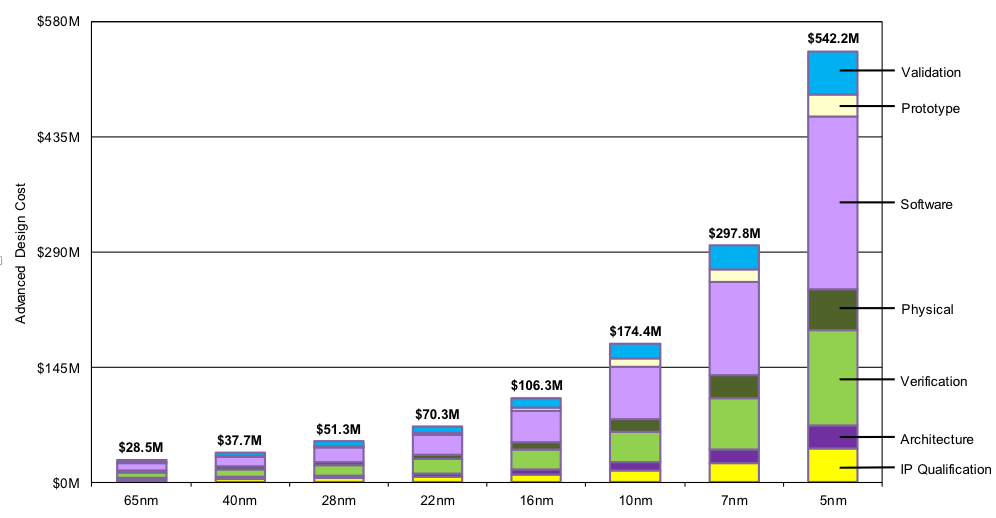
\includegraphics[width=0.99\textwidth]{figures/nre-cost.png}
    \caption{Early design non-recurring engineering~(NRE) cost
    at various feature dimensions. Source: IBS.}
    \label{fig:chip-nre}
\end{figure}

Part of the problem is that there appears to be no silver bullet for reducing
ASIC NRE, as there many disparate sources that often span multiple domains of
chip design~(Figure~\ref{fig:chip-nre}). Instead, we will need many diverse
tooling improvements united under a reimagined methodology for building custom
silicon. At Berkeley, we have articulated one such vision inspired by agile
software-engineering practises~\cite{AgileHW} and have built tools to support it.
These tools include Chisel~\cite{Chisel}, a more productive hardware-design
language (HDL) based in Scala, and FIRRTL~\cite{FIRRTL}, a flexible
intermediate representation for hardware that makes it easier to build
compilers. Perhaps the largest contribution to this vision has been the RISC-V
instruction set architecture~(ISA)~\cite{WatermanDissertation}.  Being open and
free-to-use, RISC-V enables chip designers to build customized microprocessors
while extending an open-source software toolchain.  This avoids the costs and
legal encumbarances of using a priopreitary ISA, or the massive engineering
burden of developing a fully custom ISA. RISC-V adoption has been meteoric in
recent years, both in academia outside of Berkeley~\cite{BlackParrot, Celerity,
Pulp}, and in industry, where a growing body of companies, notably SiFive,
Western Digital, and Nvidia have been developing new RISC-V implementations.

One unaddressed deficiency in chip design that drives verification, validation and software development
costs, is the lack of a good full-system simulation technology. Ideally, such
a technology would be:
\begin{itemize}
    \item \textbf{Fast.} As fast as silicon prototype, so as to enable running full system
    stacks and complete applications.
\item \textbf{Detailed.} It would simulate SoC's timing characteristics exactly.
\item \textbf{Productive.} It would be easy to debug and fast to recompile.  It would feel much like a software-based simulator.
\item \textbf{Inexpensive.} It would be cheap to deploy so that it could be made widely accessible
        to hardware and software design teams and support running large parallel experiments.
\end{itemize}

In practise, existing simulation technologies are forced to prioritize two of
these objectives. Software simulators, despite being easy to use and relatively
inexpensive, are much too slow to run full-system simulations when providing a
cycle-accurate model of the chip. For speed, chip designers are forced to turn
to hardware acceleration, in the form of FPGA prototyping and hardware
emulation.  Of the two, FPGA prototypes tend to be faster and less expensive,
and so see extensive use in software development and regression testing later
in the design cycle.  Conversely, hardware emulation is slower and considerably
more expensive, but offers a software-simulator-like debugging experience that
makes it a critical tool for pre-silicon verification. We will expand more on these
differences in Chapter~\ref{sec:simulation-background}.

The central question of the simulation work underway at Berkeley asks if it is
possible to build a simulation platform that can marry the speed of FPGA
prototyping, and the productivity of hardware emulation, while being radically
cheaper to deploy. Such a technology would put hardware emulation in the hands
of smaller research groups, and make it more widely available in companies
where scarse emulation resources must be carefully scheduled. Additionally, if
it is fast enough, it could subsume the role of a conventional FPGA prototype,
reducing the engineering burden of having parallel emulation and FPGA
prototyping infrastructures. If this technology is going to be inexpensive, two
things are clear.  First, it must use commericial off-the-shelf~(COTS) FPGA
platforms, and not custom devices or system integration as is true of all
commerical emulators. Second, this technology's software ecosystem, including
tools and IP libraries, will need to be open-source with the hope that they can
be developed and maintained by a community of users instead of a private team
of engineers.

This is no small undertaking but one made easier by recent technology trends.
Firstly, modern FPGAs are enormous, continue to be amoung the greatest
beneficiaries of Moore's law since they can naturally scale to use larger
transistor budgets. Advances in multi-die integration technologies have made
it easier to reliably manufacture even larger FPGAs. This makes it possible to
simulate considerably larger systems on a single FPGA.  Secondly, FPGAs are now available
in public cloud and provided by many major vendors like Amazon Web Services~\cite{amazonf1}.
This means a team can avoid the expense of building and
maintaining their own local FPGA cluster, and can use newer FPGAs as they
become available. Cloud services also provide an elastic supply of FPGAs,
allowing users to scale out experiments as needed, instead of needing to
provision a local cluster for the worst case. While the rates of using
cloud-based FPGAs are currently non-trivial, we expect these to fall in the
future as the costs of these services are amortized. Finally, it would be
difficult to build out an emulation infrastucture without the aforementioned advances in
open-source tooling. A compiler lies at the heart of all hardware emulation systems:
FIRRTL and its and Scala-based compiler infrastructure provide flexible
abstractions for translating a design into an FPGA-hosted emulator. FPGA-hosted emulation
infrastucture requires customized hardware, and more productive hardware-design
languages, like Chisel, makes it considerably easier for a small team to build
it. Finally, for an open-source infrastructure to see use, it
requires open-source input designs to both encourage adoption and inform
development. Here, we can leverage a growing body of RISC-V based processors,
such as Rocket~\cite{RocketChip} and BOOM~\cite{BOOM}, to feed into our system.

While it initially began as a project to study warehouse-scale computers, the
FireSim~\cite{FireSim} project has been our attempt at building out this
new technology. FireSim has been the basis for a
number of emulation-related research papers at Berkeley: we have studied
detailed DRAM timing models~\cite{FASED}, non-invasive, full-system profiling
techniques~\cite{FirePerf}.  FireSim-adjacent projects, using the same
underlying compiler, MIDAS~\cite{MIDAS}, have explored novel techniques for rapid
debugging~\cite{DESSERT}, and energy estimation~\cite{Simmani, Strober}. Over
time, features from these projects have gradually been integrated in mainline
FireSim, where they are employed by a growing user base.

Unfortunately, limitations with MIDAS limited its scope
to simple designs. First, these designs were small: they could be directly
implemented on a single Xilinx Ultrascale+ VU9P FPGA. In contrast, FPGA prototypes
of modern SoCs require partitioning over multiple FPGAs~\cite{FPMM}.  Second, these systems possessed only a single
clock domain. Conversly, modern SoCs have dozens of clocks whose frequencies
may change during execution. Without the ability to simulate
even a small number of fixed-frequency clocks it was difficult to get truly
accurate performance estimates with FireSim. Addressing these two challenges
drove the design of a new optimizing-compiler called Golden Gate~\cite{GoldenGate}.

To simulate larger systems, Golden Gate uses multi-cycle resource optimizations
to replace FPGA-hostile blocks. Golden Gate automates many techniques
deployed in prior academic work in FPGA-accelerated microarchitecture
simulation to radically improve the capacity of single FPGA. These
optimizations are the focus of Albert Magyar's dissertation~\cite{MagyarDissertation}.
Addressing the second challenge of simulating systems with more realistic clock
organizations is the subject of this dissertation. The contribution of this
work are threefold:

\begin{enumerate}
\item We describe Golden Gate, an optimizing compiler infratructure to deploy module-based
    multi-cycle resource optimizations~(Chapter~\ref{sec:golden-gate}. This
    contribution is shared with Albert Magyar, and is also described in his
    dissertation.

\item A simple, FPGA-flexible, extension to Golden Gate to support systems
    with fixed frequency clocks that is compatible with multi-cycle resource optimizations~(Chapter~\ref{sec:static-multiclock}).

\item A general, distributed approach for simulating clock generating and switching structures,
    based off of  prior work in software parallel discrete-event
    simulation~(Chapter~\ref{sec:dynamic-multiclock}). As above, our
    implementation co-exists with all multi-cycle resource
    optimizations.
\end{enumerate}

All of the software described in this dissertation is open source. We make
frequent reference to specific versions of the FireSim codebase to provide more
context in each chapter. Code references will use \texttt{monospace typeface}
where applicable. We hope this will help document features of FireSim as more
users adopt it. At time of writing, Golden Gate and support for fixed-frequency
clocks~(Chapter~\ref{sec:static-multiclock}) have been integrated into mainline
FireSim and are under active use. The features described in
Chapter~\ref{sec:dynamic-multiclock} are tagged \texttt{pdes}, and will be
merged in the future.

\section{Previous Publication, Collaboration, and Funding}

Portions of this work were published at the 2019 International Conference on
Computer-Aided Design as ``Golden Gate: Bridging The Resource-Efficiency Gap
Between ASICs and FPGA Prototypes'', though in this dissertation we focus on
the design of the compiler. The specific resource optimization employed in that
publication is described at length in Albert Magyar's dissertation~\cite{MagyarDissertation}.  Early results
from our initial support for emulation of multiple fixed-frequency
phase-aligned clocks, were published as ``Accessible, Resource-Efficient
FPGA-Accelerated Emulation Using FireSim'' in a July 2021 IEEE MICRO special
issue on FPGAs in Computing.

Donggyu Kim drove the bulk of MIDAS development based on his work on
Strober~\cite{Strober}. In the ``1.0" version of MIDAS presented in his
dissertation~\cite{DGKDissertation}, I contributed the design of endpoint
system. The final version of that compiler used by FireSim is described in
Chapter~\ref{sec:fpga-des}.

The work uses features developed by other FireSim contributors. Notable
contributors include Alon Amid, who developed much of the debug infrastructure,
Howard Mao, who has contributed to nearly all subsystems in FireSim, and Sagar
Karandikar, who ported MIDAS to use AWS and designed the cloud manager.

Finally, Golden Gate was the product of a tight collaboration between myself
and Albert Magyar. Much of the complexity in our dissertations is tied to the
FIRRTL-based software instructure required to analyze target SoCs and transform
them into latency-insensitive networks. This common infrastructure is described
at length in Chapter~\ref{sec:golden-gate}, and is the basis for the remainder
of the disseration.

The information, data, or work presented herein was funded in part by the
Advanced Research Projects Agency-Energy (ARPA-E), U.S. Department of Energy,
under Award Number DE-AR0000849.  Research was partially funded by ADEPT Lab
industrial sponsors and affiliates Intel, Apple, Futurewei, Google, and
Seagate.  The views and opinions of authors expressed herein do not necessarily
state or reflect those of the United States Government or any agency thereof.



%\chapter{Anatomy Of A Modern SoC}
%
%% in this section we review the design of a modern SOC with particular focus on
% it's clocking and reset structures, to motivate the design of our simulation
% infrastructure described later in this dissertation.

% Intro paragraph: Leave to introduction.
% - Talk about size
%  - 2.5 - 3D integration
%  - Give examples of large GPUs, CPUs
% - Heterogeneity
%   - Talk about specialization
%
% Combination of enormous size and increasing heterogenity leads to more complex
% clocking structures. Jump into this section assuming this has been established.
%

%  Overview of clock use in a modern SoC
%  - GALs
%  - Example SoC (eagle)
% Section: Clock domain crossings
% - Metastability, synchronizer chains
% - Fully asynchronous crossings
% - Rational crossings
% - Other types; see Ben Keller
% Section: Clock generation and selection structures
% - Clock Muxes
% - Clock Dividers
% - PLLs and DLLs
% Section: Reset sequences
% - How does a chip come out of reset, how do the clocks come up. Ordering considerations.
% Section: Clock gating
% Section: Dynamic frequency scaling
% - Explain what and why (DVFS)
% - Refer back to previous section RE: how clocks are reconfigured
% - Given an example system from Berkeley
% - Study an example system from not berkeley
% Clocks and EDA
% - SDC


\chapter{Full-System Simulation of SoCs}

Full-system simulation is used ubiquitously in SoC design and verification. We commence this chapter
with an exploration of the roles served by full-system simulation
in the SoC design process, and discuss commonly used full-system
simulation technologies with emphasis on hardware-accelerated forms like FPGA
prototyping and hardware emulation. From there we pivot to study how computer
architecture researchers employ full-system simulation to conduct higher-level
architectural and microarchitectural studies, and how academics have sought to
use FPGAs to accelerate these simulations.
We conclude the chapter by reviewing work done by the Berkeley Architecture
Research~(BAR) group over the past decade that attempts to build more
cost-effective hardware emulators by applying techniques from these
FPGA-accelerated microarchitecture simulators as automatic transformations to
SoC RTL.

To avoid confusion when speaking of computers simulating computers, the
literature commonly makes a distinction between the \emph{target}, the system
being simulated, and the \emph{host}, the system
executing the simulation. The host is often not a single machine but
a collection of interconnected machines, which may include CPUs,
GPUs, and FPGAs.

\section{A Tour of Full-System Simulation for SoC Design}

Simulation is central to performing three fundamental tasks of SoC design.

\begin{enumerate}

    \item \textbf{Prototyping:} ``What thing should we
        build?" Prototyping serves as a means to rapidly evaluate different
        design points with an imperfect model of a proposed design.

    \item \textbf{Verification:} ``Did we build the thing right?" Verification
        serves to check, or prove, that a particular implementation
        correctly executes.

    \item \textbf{Validation:} ``Did we build the right thing?" Validation
        serves to show that the implementation fulfills the objectives set out
        for the system.

\end{enumerate}

Both prototyping and verification can be applied at all levels of the design
hierarchy.  For example, given a specification of the system into which an
accelerator is integrated, one could prototype different design points and
verify an implementation of that accelerator. Validation, however, seeks to
answer a system-level question that spans the entire computing stack.  The
surest way to validate a system is not in simulation, but at-speed with a
physical prototype or the final product itself. However, waiting for a silicon
prototype pushes validation late into the design cycle making it challenging or
impossible to pivot the design of the system based on validation results. To
perform \emph{pre-silicon} validation, a fast and accurate full-system
simulator is required.

Here, SoC designers are confronted with a fidelity-performance-cost trade-off,
and are forced to use multiple different simulation technologies at different
points in this space. A summary of these technologies can be found in
Table~\ref{tbl:full-system-simulation-tech}.

\subsection{CPU-Hosted Simulation for Prototyping}\label{UArchSWSim}

Architecture-level simulators such as QEMU~\cite{QEMU}, which model the system at the
instruction-set-architecture level and include as limited set of standard
device models for I/O, are fast and inexpensive as they run on conventional CPUs.
When augmented with simple timing models, they are ideal for doing initial system prototyping, as
these models can be quickly modified and recompiled.
However, as these timing models become more complex, they become more
challenging to validate, and crucially, the throughput of these simulators rapidly declines.

Continuing in the direction of increasing fidelity, microarchitecture-level
simulators such as Gem5~\cite{Gem5}, and MARSSx86~\cite{MARSSx86}. are CPU-hosted 
simulators that provide configurable, ``cycle-level" timing models of a complete systems, including CPU pipelines,
caches, and off-chip memory systems.  These simulators can run target workloads at hundreds of KIPS, but are
often much slower in practice when employing more detailed or custom models. This
makes it practically impossible to run complete workloads, such as
multi-threaded Java applications or SPECint2006~\cite{SPEC2006} with its reference
inputs. Here, a common remedy is to employ statistical sampling
techniques~\cite{smarts} to fast-forward to the region of interest on an architecture-level simulator, before
executing O(100M) instructions at the desired fidelity.

While this approach has well-acknowledged shortcomings~\cite{gem5error},
judicious use of cycle-level simulators can be an appropriate vehicle for
doing initial system prototyping. For radical proposals that involve
aggressive microarchitectural changes or traverse multiple layers of the
computing stack, this approach is often inadequate (particularly for workloads that
are multithreaded, or are long-running and irregular, for which it is difficult to collect 
meaningful samples without perturbing the system under evaluation, such as
managed-language workloads~\cite{MicroSimPanel}).


\subsection{CPU-Hosted Simulation for Verification}

Since the aforementioned simulation techniques use abstract models of the
target system, they are useless for system verification and validation once
implementation begins. (In fact, those models will need to be validated against the
implementation as it is completed). Instead, here designers use CPU-hosted
simulators that faithfully represent the implementation at a particular
abstraction level.

For simulating digital components of the SoC, a Register Transfer Level~(RTL) ,
like Synopsys VCS, or Verilator, is the tool of choice. Broadly speaking, RTL
simulators model state elements and the combinational functions that update
them at cycle boundaries. Values on wires transition instantaneously, and in
general no delay through launching registers, combinational circuits is
modeled. Supposing the underlying digital abstraction holds, RTL simulation
ideal for doing dynamic verification of a digital circuit. Small blocks compile
in seconds, while complete SoCs can be compiled in 1s to 10s of minutes. RTL
simulators are relatively easy to debug, as they provide complete visibility
over the state of the design over the entire duration of a simulation. The
cost~(\$) of an RTL simulator comes mainly from licensing fees, as simulators
run on standard servers or desktop CPUs, though in many cases open-source RTL
like Verilator can be used instead. Ultimately, the largest challenge in using
CPU-hosted RTL simulator is that they have poor simulation throughput for large
designs. Completely SoCs execute at hundreds to less than 1 Hz -- much too slow
to do verification for all but small inputs (e.g., checking system boot), or
for doing full-system validation.

It's important to note at this point that, higher-fidelity software simulation
of the design is commonly used after the SoC is synthesized and implemented in
a particular process technology.  These simulations include combinational,
wire, and parasitic delays, and can generally include more detailed models of
analog components of the system. The additional fidelity only exacerbates the
throughput limitation of CPU-based simulation.

To do effective full-system validation and dynamic verification, considerably
faster simulation throughput is required. While there are many techniques that
can improve throughput on CPUs, such as multithreading, relaxing or restricting
the the timing semantics of the design language, ultimately the abundant
fine-grained, often bit-level, parallelism of RTL simulation cannot be exploited
by multiprocessors to overcome the 6+ order of magnitude slow down over a
silicon prototype.

\subsection{FPGA Prototyping}\label{sec:fpga-prototyping}

To build simulators that execute a rates closer to a silicon prototype, designers turned
to fine-grained parallel hardware to simulate SoCs.  The earliest form of
hardware-accelerated full-system simulation emerged in the 1980s, and used
programmable logic devices, specifically FPGAs, to directly implement the
design. This is known as \emph{FPGA prototyping}.

Modern FPGA prototypes directly implement the SoC on one or more
FPGAs, often with a custom board design that may include peripherals
identical to those that would be deployed in the final system.  FPGA prototypes
are fast: small prototypes that fit in a single FPGA execute at ones to hundreds of
MHz, while larger prototypes, which must be partitioned across multiple FPGAs,
simulate at hundreds of kHz~\cite{nehalemprototype, atomprototype}.
Often, FPGA prototypes are inexpensive enough that they be can readily
duplicated and distributed across hardware and software engineering teams.

Relative to software simulation, prototypes have greater fixed costs (to buy, design, and/or license the 
prototyping platform), but more critically, are difficult to use:
\begin{enumerate}
    \item Poor design visibility makes it difficult to debug failing systems. Users must instantiate
        FPGA specific debugging hardware which provides only a limited set of
        signals for a small window of time, as these tools consume considerable
        FPGA resources.  If the bug is not found on the first iteration, the
        process must be repeated: the design must be resynthesized with a new
        set of sampled signals.

    \item Long compile times (ones to tens of hours) make it difficult to
        iterate about a design point, and lengthens the aforementioned the debug cycle.

    \item Large designs must be partitioned across multiple FPGAs either
        manually, or with specialized tools. This makes the prototype hardware
        more expensive and decreases simulation throughput.

    \item Many ASIC structures, such as multi-ported RAMs and clock generators,
        cannot be synthesized to FPGA fabric so must be replaced with an FPGA
        equivalent.

    \item FPGA-specific I/O models are required to build out a complete system. Using hardened
        IP on the FPGA may not be a good model of the target system. Doing software co-simulation of IO
        often reduces simulation throughput.

    \item Prototypes are not natively deterministic making it difficult to
        reproduce certain classes of system failure, especially those that
        involve IO.

    \item Prototypes require a complete RTL implementation of the design.
\end{enumerate}

These limitations make FPGA prototypes unproductive for doing full-system
verification. However, in most cases FPGA prototypes are the fastest available
full-system RTL model the target and so are used extensively for
pre-silicon software development and regression testing.

\subsection{Hardware Emulation}

Hardware emulation aims to provide productive full-system verification by
marrying the speed FPGA prototypes with the usability software simulators.
Hardware emulators tend to be expensive to license and run -- millions of
dollars per unit -- making them a precious commodity that must be carefully
shared across a company.

Each of the three major CAD vendors offer hardware emulation solutions.
Mentor Veloce~\cite{Veloce} and Cadence Palladium~\cite{Palladium} are the historical market leaders in
hardware emulation, with the two often swapping positions with the release of updated
emulation platforms, with Synopsys ZeBu~\cite{ZeBu} rounding out the offerings.
Differences in the implementations of these three emulators put them at
different points in the cost-usability-performance space -- we describe these three strategies in the following sections.

\subsubsection{ASICs - Logic Processor Arrays}

Perhaps the earliest form of hardware emulation traces back to IBM research's
Yorktown Simulation Engine~(YUE~\cite{YSEHardware}) and its industrial-strength successor project
the Engineering Verification Engine~(EVE~\cite{EngineeringVerificationEngine}). These machines consisted of an array
of small processors which would simulates pieces of the DUT. Processors were
specialized for simulating logic (Logic Processors) and memory (Array
Processors), and were interconnected with high-radix crossbars (256 x 256 in
these early machines). A compiler~\cite{YSESoftware} would partition, map, and schedule
the DUT onto this array. Both EVE and YUE could do gate-level simulation in zero-delay
or unit-delay (every gate propagation incurs a constant delay) modes. Cyclist~\cite{Cyclist}
is a recent academic work that further explores this approach; it uses a
homogeneous array of custom RISC-V cores attached in a 2-D mesh network.

Cadence's Palladium~\cite{Palladium} emulators derive from EVE (which was for a time sold by QuickTurn Design Systems under the name CoBALT~\cite{CoBALT}, before they
were acquired by Cadence. Relative to
competing emulation solutions, Palladiums have lower capacity per unit, but the
fastest compile times. Palladiums also have highest power consumption and must be
water-cooled -- unlike the competing offerings.


\subsubsection{Custom FPGAs}
While a EVE-like processor arrays can provide radically improved compilation speeds since
the compilation problem is fundamentally simpler than running FPGA place and
route, one natural alternative is to modify conventional FPGAs for emulation.
This might involve adding dedicated hardware to improve debuggability (e.g., to make it
possible to capture full-visibility waveforms), adding I/O multiplexing
hardware to ease the FPGA-partitioning problem~(i.e., a hardware implementation of Virtual Wires~\cite{VirtualWires}), and modifying the programmable
fabric to better match the resources and interconnect required ASIC designs.

This is the approach taken by Mentor Graphics's Veloce~\cite{Veloce} emulation platforms.
Veloce emulators appear to have better capacity than Palladium, but slower
compile times. Veloce emulators use less power and are air-cooled.

\subsubsection{Commercial-Off-The-Shelf FPGAs}

Hardware emulation large total-cost of ownership is driven to some degree
because the leading emulators are both power-hungry and use custom silicon. To
skirt some of the costs of those platforms, a third alternative that sees
industrial use is to use large, commercial-off-the-shelf FPGAs but rely on
custom tooling and system packaging to improve usability. Synopsys's
ZeBu~\cite{ZeBu} platform does precisely this by leveraging the largest
available Xilinx FPGAs available at the time of its release (Virtex Ultrascale
VU440s~\cite{ZeBu}). At time of writing, ZeBu provides the highest simulation
throughput and the lowest power consumption but has a reduced debug feature set
relative to other emulators.

In its use of COTS FPGAs, Synopsys ZeBu is most similar to the work presented herein. 

%\begin{sidewaystable}
%\begin{center}
%\resizebox{\textwidth}{!}{%
%    \begin{tabular}{|p{0.1\textwidth}|p{0.1\textwidth}|p{0.2\textwidth}|p{0.2\textwidth}|p{0.2\textwidth}|p{0.2\textwidth}|}
%    \hline
%        \textbf{Technology} & \textbf{Examples} & \textbf{Speed}\newline(Relative to Silicon) &
%        \textbf{Fixed Cost} \newline(\$ per simulator) &
%        \textbf{Variable Cost}\newline(\$ per target-second) & \textbf{``Compile" Time}\newline(Hours)  \\
%    \hline
%    \hline
%        Arch SW Simulator & QEMU \newline Spike & $10^{-1}$ & Free + $10^3$ & \TODO{} & 0 - 0.1 \\
%    \hline
%        $\mu$Arch SW Simulator & Gem5 \newline MARSSx86 & $10^{-6} - 10^{-4}$ & Free + $10^{3}$ & \TODO{} & 0 - 0.1 \\
%    \hline
%        RTL Simulation & VCS \newline Verilator  & $10^{-7} - 10^{-4}$ & $10^{3} /seat/yr + 10^{3}$ \newline $10^{3}$ & \TODO{} & $10^{-2} - 10^{-1}$ \\
%    \hline
%        Single-FPGA prototype & FPGA-zynq & $10^{-2} - 10^{-1}$ & 2495~(ZC706) \newline 495~(Zedboard) &% \TODO{10W (ZC706)} & 0.5 - 1 (FPGA-zynq)\newline $10^{0} - 10^{1}$ \\
%    \hline
%        Multi-FPGA prototype & \cite{nehalemprototype}, \cite{atomprototype} \newline Protium S1  & $10^{-4} - 10^{-3}$ & \TODO{} & \TODO{} & \TODO{} \\
%    \hline
%        Hardware Emulation & Palladium Z1 & $10^{-3} - 10^{-2}$ & $10^{6}$ & \TODO{$10^{-2}$} & 140 MG/hr \\
%    \hline
%        Silicon Test-chip & \TODO{} & 1 & $10^{5} - 10^{7}$ & \TODO{$10^{-5} - 10^{-4}$} & $10^3 - 10^4$ \\
%    \hline
%\end{tabular}}
%\end{center}
%    \caption{Contrasting different technologies for building full-system
%    simulators; ordered approximately from top-to-bottom in descending
%    fidelity. We define ``compile time" to be the time it takes to make one
%    design iteration less the time spent in simulation and implementing a design
%    change; the time to generate a simulator from a specification of the
%    target.}
%\label{tbl:full-system-simulation-tech}
%\end{sidewaystable}%

\section{Hardware-Accelerated Microarchitecture Simulation}

In order to build more cost-effective hardware emulators, this work draws from
technologies developed in academia to accelerate cycle-level microarchitecture
simulation~(this is described see Section~\ref{UArchSWSim}).

The first, most obvious way to accelerate these is to
parallelize them over multiprocessors or networks of workstations.
One early example of this is the Wisconsin Wind Tunnel~(WWT)~\cite{WisconsinWindTunnel}, which relied
on a window-based, parallel discrete-event simulation engine to manage synchronization
across workstations. For CPU-hosted simulators like the WWT, and recent works like Graphite~\cite{Graphite}, to achieve
good performance they must reduce the synchronization overhead between
partitions of the design by either modeling the target more abstractly, or by
introducing extra target-latency between partitions.  While this may be
appropriate for building coarser models, it's ineffective for accelerating RTL
simulations and thus for building hardware emulators, which, at best, require
per-cycle synchronization.

So, in order to build simulators that were both fast and cycle-accurate
many academics turned to FPGAs, which by the 1990s and early 2000s had proven themselves as effective
vehicles for ASIC prototyping and emulation. However, instead of directly implementing an
ASIC design, here FPGAs would be used as a host for microarchitectural models written in RTL.
An early example of this approach is the Rapid Processor Emulator~\cite{RPM, RPMDesign}, however the bulk of the research
in this domain can be attributed to the RAMP project~\cite{RAMP}.

\subsection{Research Accelerator For Multiple Processors (RAMP)}

The RAMP project began in 2005 driven by the realization that advances in computing performance
would require exploiting other forms of parallelism beyond ILP, as the end of
Dennard scaling would necessarily make single-threaded performance improvements
more difficult to attain. The goal was to develop a shared full-system
simulation infrastructure for the computer architecture community which would
be better suited to study future thread-parallel systems of 64 - 1024
processors, than traditional software simulators. Member universities included UT
Austin; CMU; UC Berkeley; University of Washington; Stanford; and MIT.
%While
%the RAMP project ultimately failed to produced a unified simulation
%infrastructure, differences in the the simulators produced by the member
%institutions each uniquely advanced the state-of-the-art.

At the onset of the project three initial, monolithic prototypes were built,
each was designed to model a different class of target.
RAMP Red, later known as ATLAS~(Stanford)~\cite{ATLAS} was designed to study transactional-memory-based chip-multiprocessors, and supported up to 8 PowerPC cores.
RAMP Blue~(UC Berkeley)~\cite{RAMPBlue} was tailored for large-scale distributed-memory message-passing machines and used Xilinx
Microblaze softcores to prototype the target system. Partitioned over 21
BEE2 boards, RAMPBlue could simulate a system with as many as 1008 cores.
Finally, RAMP White~(UT Austin)~\cite{RAMPWhite} modeled cache-coherent
shared-memory processors. It supported both PowerPC (when using a Xilinx
host with a hardened PowerPC 405 core) and 32-bit SPARCV8 (soft core) targets.
Each of these prototypes used the same host platform (the Berkeley Emulation
Engine 2)~\cite{BEE2}, and were initially constructed using shared libraries and a common
specification language called the RAMP design language~\cite{RDL}.

Other, mostly later, projects tied to RAMP abandoned the shared infrastructure
and explored different simulator design styles.
ProtoFlex~(CMU)~\cite{ProtoFlex} was an architecture-level simulator that
demonstrated 16-way host-multithreading of a single FPGA-hosted functional
model.  ProtoFlex could switch between FPGA-hosted and CPU-hosted modes via
a process it called transplantation. FAST~(UT Austin)~\cite{FAST} was a cycle-accurate
x86 simulator which leveraged a split, CPU-hosted functional model and FPGA-hosted
timing model. RAMPGold~(UC Berkeley)~\cite{RAMPGold} used FPGA-hosted timing
and functional models with 64-way host-multithreading to realize a larger
target on a single FPGA.  To model a datacenter-scale target,
DIABLO~(UC Berkeley)~\cite{Diablo} stitched together 24 instances of a modified version RAMPGold to simulate 3072 interconnected
servers.  Finally, HASim~\cite{HASim}(MIT) also used FPGA-hosted timing and
functional models, but provided more detailed pipeline and memory hierarchy
models. Later work studied partitioning HASim over multiple FPGAs~\cite{LIFPGADesign} and showed that by using two FPGAs HASim could host eight
times as many cores, due to improved resource sharing between virtual
instances.

Around the same period, other groups not associated with the RAMP project explored
using FPGAs for microarchitecture simulation.  One notable example is
DART~\cite{DART}, an FPGA-based Network-on-Chip simulator that used
multithreading, like many RAMP simulators, but leveraged NoC-specific model abstractions
to permit a wide range of runtime-reconfigurable model parameters.

\subsection{FAME Taxonomy}

One output of the RAMP project was the FPGA Architecture Model
Execution~(FAME)~\cite{FAME} taxonomization of FPGA-accelerated simulation work,
which distills many of the contributions of the works above into three
dimensions: host-decoupling (FAME-1), abstract RTL vs concrete RTL (FAME-2),
and multithreading (FAME-4). In practise, simulators employing multithreading
tend to be host decoupled --- under this taxonomy, these would be referred to as
FAME-5 simulators. Similarly, RAMPGold~\cite{RAMPGold} and HASim~\cite{HASim}
are FAME-7 simulators: they deploy all three techniques.


\subsection{FAME-1: Host Decoupling}\label{sec:fame1}

In host-decoupled FPGA simulators, a target cycle of simulation
executes over multiple FPGA-host cycles. In contrast, a
conventional FPGA prototype executes a single target-cycle on every FPGA-host
cycle; multiple clocks can be prototyped using multiple host clocks with the
same relative frequency relationship as exists in the target.
With host-decoupling, ASIC structures that map inefficiently to FPGA fabric may be replaced
with optimized-for-FPGA structures that take more host cycles to execute, but save
FPGA resources and improve host-cycle time.  One classic optimization replaces
multi-ported register files and CAMs with a dual-ported BRAMs pumped over
multiple cycles.  Additionally, host-decoupling permits the simulator to
tolerate variable latencies in the host without sacrificing simulator
performance or changing the target-time behavior of the simulation.
Nearly all academic FPGA-accelerated simulators employ host-decoupling.
Unlike FPGA prototypes, commercial FPGA-based emulators are necessarily host-decoupled to
make them execute deterministically and to support a wealth of additional features that may require
halting parts of the emulation. We expand on mechanisms for implementing host-decoupling in Chapter~\ref{ch:fpga-des}.

\subsection{FAME-2: Abstract RTL}

In an abstract-RTL FPGA-accelerated simulator, components of the simulator do
not model the implementation RTL exactly. Abstraction permits simplifying
components of the target, trading simulation fidelity for FPGA-resource
savings. Additionally, abstract models can be made reconfigurable in ways the
implementation RTL cannot~(e.g., a latency-pipe model can expose its latency
as a runtime-programmable register).  The FAME-2 dimension of the taxonomy
represents a spectrum in practice.  Most academic FPGA-accelerated simulators
are either partially or completely abstract-RTL simulators.  Even commercial
hardware emulators and FPGA prototypes are to some extent abstract --- as
generally some ASIC features may need to be replaced with an equivalent model
provided by the emulation or prototyping platform.
%Can i cite documentation?

\subsection{FAME-4: Multithreading}

In a multithreaded FPGA-accelerated simulator, like HASim or RAMPGold, multiple virtual instances of a
block or module within the target are simulated using a single physical
combinational datapath on the FPGA. The target state is duplicated according to the number of
virtual instances, and a scheduler selects which virtual instance should be
simulated in a given host-cycle. ASIC logic tends to be expensive when mapped
to FPGA fabric; in FPGA prototypes, designs tend to be logic~(LUT) constrained,
which leaves much of the FPGA's embedded BRAM left unused.  Multithreading
improves the mapping efficiency of the target, by reusing the expensive logic
over multiple copies of target state which can be mapped into abundant FPGA BRAMs and registers.
To the best of our knowledge, commercial hardware
emulators and FPGA prototypes do not use multithreading schemes for sub-components of the target.

\subsection{RAMP Retrospective}

Ultimately, RAMP-style FPGA-accelerated simulation failed to take off
in the computer architecture community. There are a number of technical explanations for this, though many of these
derive from the aforementioned challenges with using FPGAs to prototype ASICs~(see Section~\ref{sec:fpga-prototyping}).
Three more specific challenges include:

\begin{itemize}
    \item \textbf{Large Relative Barrier to Entry.} Open-source software simulators can run on machines researchers already possess,
whereas FPGA-based simulators requires expensive hardware. For instance, the early RAMP prototypes all used
the BEE2 board. While using smaller, more inexpensive boards would reduce initial capital costs, it does so at the expense of reduced simulation capacity.
Simulators using smaller hosts, like RAMPGold, required extensive resource-optimizations to support simulating research-worthy target designs.

\item \textbf{Reproducibility of Results.} Since RAMP simulators were tied to particular FPGA host
platforms, other researchers would need to purchase the same host to reproduce
publish results. Even if researchers had access to their own FPGAs, they
generally could not run a simulator designed for a different host on their own
FPGAs without modification to simulator.

\item \textbf{Modeling Complexity.} Designers of RAMP simulators have said that
designing models was more difficult than writing RTL for the matching implementation.
Consider a processor pipeline: to model detailed ``cycle-accurate" behavior of that pipeline
the model designer must write RTL that contains much of the same complexity inherent to the actual pipeline's design in order
to properly capture the all hazards that may affect the processors performance.
In order to support modeling a space of different processor designs, either at compile time by generating different model RTL, or at runtime
, by adding logic to permit reconfiguring the simulator, they must add still more complexity.
In order to provide reasonable simulation capacity, they must also apply multi-cycle resource optimizations to the model.
Taken together, this complexity makes the model more difficult to debug than an already-difficult-to-debug FPGA prototype,
and to add insult to injury, these models, like their software counterparts, must still be validated against a real implementation.
\end{itemize}

%
%\section{FAME-1 Target Dataflow Abstractions}\label{sim:fame1-abstractions}
%
%* Another product of the RAMP project and follow on works, were FPGA-friendly abstractions 
%for describing target designs so that they could be easily host-decoupled.
%
%* At a high level, these abstractions represent the target as a dataflow graph of actors. The execution
%of this graph defines a deterministic simulation of the target it represents. These actors can be hosted
%
%* In essence this represents a simplification of conservative Parallel Discrete Event
%Simulation, we will cover this in a later chapter.
%
%in software or on the FPGA -- he
%
%* RAMP model
%  * Used in RAMPGold
%
%* APort Networks
%  * Used in HASim
%
%* Deadlock Avoidance
%
%* LI-BDN


\section{Recent Work at Berkeley}\ref{sec:ucb-bar-recent-work}

At the end of the RAMP project it was clear that writing performance models for
FPGAs was not going to be tractable without major breakthroughs in improving
FPGA usability. Since evaluating an RTL implementation with an EDA flow is still
required to meaningfully assess a design's quality-of-result~(QoR), notably its critical path
delay, effort spent writing FPGA performance models would be better spent
writing the implementation. If the RTL design process could be made more productive,
computer architecture researchers may be more willing to conduct
microarchitecture studies using realizable RTL designs instead of software
simulators. In this model, once an RTL implementation is ready it could be
transformed into a RAMP-like simulator using a \emph{FAME compiler}. This circumvents the aforementioned model complexity challenge,
as these simulators would essentially be area-optimized hardware emulators of the design:
they would exactly represent the input design's behavior and so would not need
to be validated against silicon.

This was one vision that drove research done by UCB-BAR over the past decade.
To address the RTL design productivity challenge, we developed
Chisel~\cite{Chisel}. Chisel, an RTL design language hosted in Scala, allows
designers to specify rich hardware generators by leaning on the host language to provide
powerful metaprogramming features not available in SystemVerilog or VHDL.
Instead of performing parameter sweeps in a software model, with a generator
the user explores the design space by elaborating and evaluating different
\emph{instances} of the design. The Rocket Chip SoC generator~\cite{RocketChip} is one example of this: it generates complete RISC-V SoCs including
core pipelines, private caches, uncores, and common periphery devices. Rocket
Chip lets the user stitch together near-arbitrary networks of disparate devices
using it's diplomacy~\cite{Diplomacy} library, developed by SiFive, which leverages Scala's type
system to provide intelligent, area-optimized system integration. The
Berkeley Out-of-Order Machine (BOOM)~\cite{BOOM} and Hwacha vector-fetch
processor~\cite{Hwacha} Chisel generators provide additional core IP that can be
integrated into a Rocket Chip SoC.

To support writing reusable compiler transformations on generated instances, in
Chisel3, Chisel2's internal representation~(IR) of an RTL circuit and its
lowering transforms were replaced with FIRRTL~(Flexible Intermediate
Representation For RTL)~\cite{FIRRTL} and its Scala-based compiler. During
elaboration, Chisel3 emits a high-level form of FIRRTL. The FIRRTL compiler
then lowers the instance to Verilog while scheduling user-provided passes. These passes can be used to
a tailor an instance to a particular backend: for instance, when preparing a
design for an ASIC implementation, FIRRTL memories can be replaced
black boxes corresponding to technology-specific SRAMs. Alternatively, if the same
design is destined to become an FPGA prototype, these memories could be double-pumped
to save FPGA resources.

\subsection{Strober and MIDAS}\label{sec:midas-intro}

The first FAME-compiler-like work done at UCB-BAR can be found in the
Strober~\cite{Strober} energy modeling project. While
gate-level-simulation-driven power estimation using commercial tools like
Synopsys PrimeTime PX provides accurate pre-silicon results, gate-level
simulation runs much too slowly to conduct system-level microarchitectural studies using
complete workloads. Instead, Strober generates an accurate average power
estimate by sampling the execution of the workload running on a fast,
FPGA-based simulator and then replaying those samples for short durations in
gate-level simulation. By selecting an appropriate number of samples, average
power dissipation for the SoC can be estimated within a desired error bound.

To realize this, Strober needed to automatically generate an FPGA-based
simulator from ASIC RTL with ability to capture complete RTL state snapshots
and IO traces~\footnote{While these features are available in commercial
emulation tools but no reusable open-source flow existed at the time.}.
Since Strober predated FIRRTL, it modified the Chisel2 backend to:
\begin{enumerate}
    \item Host-decouple input RTL to support halting the simulator to capture
        state snapshots. This is called a \emph{FAME-1 transformation}.
    \item Inject a shadow scan-chain to read out target state.
    \item Elaborate a simulation wrapper around the transformed target. This
        wrapper included IO channels that can buffer a limited IO trace, a
        latency-pipe timing model for the target's DRAM memory system, as well
        as a simulation control bus.
\end{enumerate}

Strober simulators are co-hosted over an FPGA and an CPU -- a \emph{driver}
process, writes to memory mapped registers accessible on the simulation control
bus to advance the simulator and to initiate state snapshot capture.

Initially independent of Strober, MIDAS began as class project to build an
FPGA-based performance simulation framework. It had its own FAME-1 transform,
and a nascent library of more detailed memory system models~(this would later
become FASED~\cite{FASED}).  Seeing an opportunity to reuse work, we merged
these two projects. MIDAS, as presented at CARRV2018~\cite{MIDAS}, retained all
of Strober's features, but used Chisel3 and FIRRTL, vastly improved simulation
performance, made it easier to support co-simulation of other IO models.

MIDAS was the basis for a number of research projects at UCB-BAR. To improve simulator debuggability, DESSERT~\cite{DESSERT},
leveraged MIDAS's state snapshotting features to perform
\emph{ganged-simulation}. Here one instance of a simulator runs ahead of a second lagging instance, to
detect a simulation error. A detectable error could be either fired hardware assertion, which had been synthesized by the source FIRRTL, or a
commit-log mismatch between the target processor and an online golden model.
On detection of an error, the leading instance instructs the lagging instance to capture a
state snapshot of the target before the error would occur.  Using the replay feature, a
full visibility waveform of the failing target design could then be generated. While
commercial emulators provide rich sets of state-snapshotting features --
DESSERT's differs in that uses two simulators, to let the simulation advance at
full-throughput to the point of failure. Simmani~\cite{Simmani} revisited power
estimation, but instead of using complete state snapshots, injected
a statistically selected set of performance counters into design. These counters
could provide a dynamic estimate of power dissipation. Finally,
MIDAS's DRAM memory models were published as FASED~\cite{FASED}, we cover FASED
in greater detail in a later chapter.

\subsection{FireSim}

As Strober was being developed, UCB-BAR continued to study new architectures for
warehouse-scale computers, notably as part of the FireBox~\cite{FireBox} project.
FireBox was an early example of a disaggregated datacenter that relied on
high-bandwidth photonic networking made possible with relatively inexpensive
silicon-integrated photonics, a focus of earlier work done by the lab.  To
simulate FireBox, we built FireSim~\cite{FireSim}. Building on DIABLO, FireSim interconnected MIDAS-generated
simulators with a distributed, CPU-hosted network model to build a
cycle-accurate, warehouse-scale computer simulation. To overcome the usability
challenges of DIABLO, FireSim relies extensively on automation.  Instead of
using a custom host platform, FireSim uses the public cloud, specifically
Amazon Web Service's Elastic Computer Cluster~(EC2).  When the user wishes to run a simulation, FireSim's \emph{manager} program
requests as many FPGAs nodes (to host
Rocket Chip-derived simulators) and compute nodes (to host switch models) as required. The manager's ability to dynamically spin up and tear down simulators
deployed to EC2 to make it easy to coordinate simulations of arbitrary size. Armed with this flexibility, in our
ISCA2018 publication~\cite{FireSim} we were able to reproduce behaviors observable in real
datacenters at a variety of different simulation scales.

Since the 2018 ISCA publication, FireSim has evolved to become a
general-purpose hardware emulation environment for Rocket Chip-based SoCs. By
optionally removing the network simulation, the manager can instead batch out
parallel workloads to multiple independent simulator instances, making it
productive for doing performance evaluations of SoC-scale systems.
Presently, In addition to the manager, FireSim provides:
\begin{enumerate}
    \item A FAME compiler to generate an emulator from FIRRTL. Initially, this
        was MIDAS, but as of version 1.6.0 it has been replaced with Golden Gate~\cite{GoldenGate}.
    \item Device libraries for modeling periphery devices commonly integrated
        into Rocket Chip SoCs including a block device, UART,
        and tether model in addition a NIC model used to perform networked simulation.
    \item FireMarshal, a utility to automate building Linux distributions for
        running on RISC-V based platforms.
    \item Many of the most commonly used RTL libraries in the Rocket-Chip ecosystem, to enable the user to build out interesting systems.
\end{enumerate}

FireSim has been used both in academia and industry, primarily for doing
performance evaluations of new microarchitectural features implemented as
extensions to Rocket Chip.  At Berkeley, FireSim was the basis for
FirePerf~\cite{FirePerf}, which introduced improved instruction tracing, and
non-invasive performance counter integration to perform rapid hardware-software co-design of the NIC
and the Linux networking stack. These features have since been integrated into
mainline FireSim. Academically, FireSim has been used for microarchitectural performance evaluations,
and commercially, it has seen use at Intensivate, Esperanto, and SiFive. FireSim is also being used a RISC-V platform in DARPA's
FETT~\cite{FETT} bug bounty program~\cite{FireSimFETT}.

As a final note, in 2020 we released Chipyard~\cite{Chipyard}, which unifies all of
UCB-BAR's SoC design tools and IP under in a single environment. In Chipyard,
FireSim is a library for doing hardware emulation -- many stand-alone utilities
that were previously hosted in FireSim but aren't strictly related to hardware emulation
support, such as FireMarshal, have been hoisted up into into Chipyard,

\section{Motivations for Golden Gate~(MIDAS II)}

As adoption of FireSim started to increase, it was clear that limitations with
its FAME compiler, MIDAS, prevented it from seeing more widespread use. Firstly, MIDAS's existing FAME-1
transform supported systems with only a single, fixed-frequency clock domain,
and barred use of asynchronous resets. This precludes
simulating most realistic systems and made it challenging to validate FireSim
against existing RISC-V silicon. Secondly, capacity challenges with EC2
FPGAs made it difficult to simulate larger systems, notably the test-chips
UCB-BAR was designing concurrently. Without the ability to do multi-FPGA
partitioning, and without any automated application of RAMP-style
optimizations, this hamstrung FireSim to supporting only relatively small
SoCs. Taken together, these restrictions kneecapped FireSim to being a limited, albeit
open-source, hardware emulation environment for primitive Rocket Chip-based SoC designs.

To address these two concerns, we set about designing a new FAME compiler
called Golden Gate~\cite{GoldenGate}. Before we expand on the initial
implementation of Golden Gate, in the next chapter we review different target formalisms and
implementation strategies for building FPGA-hosted, discrete-event simulators.


\chapter{On The Design of FPGA-Based Discrete-Event Simulators}\label{ch:fpga-des}

% Survey of existing FPGA-based discrete event simulators, and their
% microarchitectural design.

For the purpose of this dissertation, it is insightful to classify FPGA-based
RTL simulators along two dimensions. For simplicity, here we consider only
single-FPGA hosts, but we note that this discussion can trivially extended to
multi-FPGA hosts. This chapter was heavily influenced by dicussion in Pellauer
and Vijayaraghavan et al. in \emph{A-Port Networks: Preserving the Timed
Behavior of Synchronous Systems for Modeling on FPGAs}~\cite{APortNetwork}.

The first dimension is timekeeping strategy. \emph{Explicit timekeeping}~(ET)
simulators, keep track of simulation time whereas simulators with implicit
timekeeping (IT) instead rely on target-cycle count as a proxy. Implicit timekeeping represents an
implementation optimization as additional FPGA resources required track and
manage timestamps are unneeded. For this optimization to apply broadly across
the simulator, target system clocks must have fixed frequency and phase, and
all simulation events must be synchronous to these clocks.

The second dimension is control granularity. At one extreme there exist
simulators with \emph{centralized control} (CC). These track time in
a single location; the entire simulator advances in lockstep from
timestep to timestep.  Conversely, there are simulators with \emph{distributed
control}~(DC). These simulators are parallel systems that can be described as a directed graph of \emph{logical
processes}~(the nodes of the graph). Logical processes~(LPs) communicate by sending \emph{messages} over the graph's edges. 
Each LP locally tracks simulation time and can advance independently. DC
simulators can be coarse-grained, with LPs simulating core-scale components, or
fine-grained, where LPs model blocks on the scale of CAMs, RAMs, or
combinational circuits, like multiplexers.

Taking the product of these two dimensions produces four classes of simulator:

\begin{enumerate}
\item{Implicit Timekeeping, Centralized Control (ITCC)}: Simple MIDAS generated simulators*. FabScalar FPGA

\item{Implicit Timekeeping, Distributed Control (ITDC)}: RAMP simulators,networked MIDAS-generated simulators.

\item{Explicit Timekeeping, Centralized Control (ETCC)}: Unrealized, commerical emulators*. Example: Direct implementations of the verilog event queue.

\item{Explicit Timekeeping, Distributed Control (ETDC)}: Multi-FPGA commerical emulators*, This Work
\end{enumerate}
\TODO{Citations here}

For all intents and purposes, DC simulators are FPGA-hosted, parallel
discrete-event simulators.  Parallel, discrete-event simulation~(PDES) has been
a vibrant area of research since the 1980s, but PDES researchers have focussed
nearly exclusively on non-FPGA hosts (including multiprocessors, GPUs,
supercomputers, networks thereof).  In the next sections, we briefly introduce
relevant PDES work, and explain how prior work in that field translates to
hosting DC RTL simulators on FPGAs. First, we explore some
CC simulator designs to help motivate the use of DC simulators despite their increased complexity.

\section{An Iron Law For FPGA-Based Simulator Performance}

If SoC designers turn to hardware emulation for speed, it is critical
to understand how emulator design affects throughput. For IT simulations of a target
with a single clock domain, Pellauer et al.~\cite{APortNetworks} present a simple performance
equation which, like the iron-law of processor performance that inspired it,
breaks down the performance of a complete simulation into a product of terms:

\begin{equation}
    f_{sim} = \frac{cycles_{t}}{cycles_{h}} f_{fpga}
\end{equation}\label{eq:sim-perf}

\noindent Where,
\begin{flalign*}
    f_{sim} &= \text{throughput of the simulator (target cycles per second, Hz)}\\
    f_{fpga} &= \text{the clock frequency of the host FPGA (Hz)}\\
    cycles_{h} &= \text{the total number of host cycles over which the simulation executed}\\
    cycles_{t} &= \text{the total number of target cycles simulated}\\
\end{flalign*}

The right term of this equation, host frequency~($f_{fpga}$), is set by the
critical path delay of the simulator. Depending on the simulator's design and
the target it models, this sometimes corresponds to a critical path in the target design, but more frequently it is a path that
drives scheduling logic in the simulator itself (i.e., some part of the circuit deciding whether to
advance forward in simulation time). The left term, a ratio of host-to-target cycles, is a measure of the
microarchitectural efficiency of the simulator. In an FPGA prototype, this term is
effectively one: every host clock simulates a target clock. In
a host-decoupled simulator, in practise, it is always less than one\footnote{While it is possible to simulate multiple target cycles per
host cycle by unrolling successive cycles of execution, there is no incentive
to do so globally across a simulator, as it would double resource utilization,
and likely double the critical path delay of the simulator. In DC simulators
of target machines with multiple clock domains, it may make sense to do this
for relatively small LPs in the fastest clock domains, if the simulator is
rate-limited on those LPs.}. Given this, Pellauer et al. tend to the
more-intuitive recipricol of this term and dubbing it the FPGA-cycles-to-Model-cycles
Ratio~(FMR). We give it in Equation~\ref{eq:fmr}. Unless it can be deduced statically,
FMR is only usefully defined over a non-trivial interval of simulation execution.

\begin{equation}
    FMR = \frac{cycles_{h}}{cycles_{t}}
\end{equation}\label{eq:fmr}

As an example, consider a five-read, three-write register file modelled by an LP that
uses a dual-ported BRAM. If the LP statically schedules all eight accesses, it
will have an FMR of four. Conversly, a more clever design that dynamically
schedules accesses only if the ports are used could have lower FMR: when the register file is lightly used the FMR of the LP could
approach one, whereas when it is heavily used it would approach the static
limit of four. Continuing with
this example, one could gang together multiple BRAMs or LUTRAMs to build a more
highly ported RAM structure capable of more port accesses per cycle.
While this could reduce the statically scheduled FMR from 4 to as low as 1, it
comes at the expense of FPGA resources and, potentially, a longer simulator
critical path which may counteract the FMR improvement.

Equation~\ref{eg:sim-perf} to apply to DC simulators, we can modify it to use
the FMR of the LP that has executed the fewest number of target cycles.
However, we note that when LPs may advance only a bounded number of cycles
ahead of slower LPs in the system for sufficiently long simulation, the
equation above returns approximately the same result for all LPs.

\section{Centrally Controlled~(CC) Simulators}

When first building a simulator, it is natural to attempt to coordinate time
globally across the FPGA. It is simpler to implement, there are fewer potential
sources of causality errors, as there aren't different pieces of the simulator at different points in simulated time,
and similarly, it easier to capture snapshots of the simulated system at particular points in
time. In a system where different components of the target may take differing,
or dynamically varying, number of host cycles to execute, there are two
common approaches.  The first, is what Pelleaur et al. call \emph{unit-delay
simulation}. Here the simulator is granted a fixed $N$-host-cycle budget to
compute each target cycle, where $N$ is equal the largest possible
latency a sub-block may take to execute~(in isolation, its worst-case FMR is $N$). While simple to
implement, this will result in wasted host cycles as in many target cycles the
full $N$ cycle allocation may be unneeded.  We also note that while it's
relatively easy to provide tight bounds for models of many on-chip
blocks, like multi-ported RAMs, it is more difficult to do so for I/O devices, which may require large $N$
in the worst case, but far less on average.

Instead of selecting $N$ statically, a natural optimization one could make is to allow sub-blocks to signal when they have
finished computing. Here, a centralized controller aggregates done-signals from all
blocks in the system and steps the simulator only once all have been
asserted~(a wide and-reduction). This is called \emph{dynamic-barrier
synchronization}. While this removes wasted host idle-cycles (FMR can fall
below $N$), it introduces new control signals that often set the critical
path delay of the simulator: these signals must be routed to a central
location on the FPGA, propogated through a potentially wide and-reduction network, and then fanned out again across the FPGA.
This problem is exacerbated in modern FPGAs, like the VU9P devices used in EC2 F1, which are composed of multiple
dies~\footnote{In Xilinx parlance, each logic die is referred to as a
super-logic regions~(SLRs).}, as these control signals must use relatively
scarser and higher-delay inter-die interconnect. Additionally, the scarcity of inter-die interconnect
puts increased pressure on the router, and for high utilizations often results
in unrouted nets, and other related DRC errors.  To improve simulator
frequency, it is natural, perhaps even necessary, to pipeline these signals at
the expense of a fixed increase to FMR: unless simulation of target cycle can
be overlapped, FMR will increase by one for each additional pipeline stage. Furthermore, while
FPGAs have scaled in capacity, their logic delays and thus achievable
$f_{max}$, have seen little improvement. This increase in capacity begets
more sub-blocks, and thus a larger and-reduction
network, futher lengthening critical path of the simulator.

\section{Distributed Control~(DC) Simulators}
These trends in FPGA scaling make it necessary to decentralize timekeeping to
produce fast simulators.  Having more LPs, each of which manage fewer control
signals that routed locally, improve ${f_{max}}$ while easing the routing and
DRC challenges with centralizing control. Distributing control introduces new
challenges.  Since LPs can decouple in target time, \emph{causality errors} can
arise if LPs act on messages out-of-order. Conversely, if LPs are too
conservative in waiting for messages to arrive, are prone to deadlock.
Finally, a simulator that is correct~(it correctly models the target, and is
deadlock free), can still suffer of poor simulation performance if transmission
latency between LPs cannot be overlapped with LP execution. Designing software
algorithms that both fast and deadlock free has been the central focus of PDES
community since its inception~\cite{FujimotoPDESPrimer}.

\subsection{A Primer on PDES}

In PDES a \emph{physical process} is divided into a set of logical processes
that communciate via timestamped messages. Any one LP is it itself a discrete
event simulator, that must to process events in timestamp order~(the
\emph{local causality constraint}). These events can be triggered internally or
by messages received from other LPs.  The underlying difficulty in PDES is that
an LP may not know that it has not yet received an older message and so cannot
safely being processing another event without potentially violating the local
causality constraint. A \emph{synchronization algorithm} is reponsible for
allowing LPs to make forward progress. There are two broad classes of synchronization algorithm in PDES:
\emph{conservative} and \emph{optimisitic}.

In conservative synchronization algorithms, LPs wait to process events until
they are certain they will not violate the local causality constraint. This
conservatism is ripe for deadlock: it simply takes a cycle of LPs with one
waiting on the next. Conservative PDES overcome deadlock by requiring that LPs have non-zero
\emph{lookahead}. That is to say, output messages must only depend on input
messages that are at least lookahead seconds in the past. Armed with this,
it becomes possible to detect and resolve deadlock, or avoid it altogether.
The Chandy-Misra-Bryant~(CMB)~\cite{NullMessagesBryant, NullMessagesChandy} algorithm avoids deadlock by introducing
\emph{null-messages}. Null-messages indicate that absence up a real
message to up to until the the time of its timestamp. If an LP with non-zero lookahead, $t_{L}$, is blocked on a input whose latest
message is timestamped to time $t_{i}$, the LP must eventually issue a
null-message at time $t_{i} + t_{L}$ to each of its receivers. This may
be sufficient to unblock the receiving LP, resolving the deadlock risk. Failing that, the receiving LP too is compelled to
send null-messages still further in the future and the process repeats.
So long as there exists no cycle of LPs with zero lookahead, the CMB algorithm
is garuanteed to avoid deadlock; for a complete proof we refer the interested reader to Chandy and Misra~\cite{NullMessagesChandy} .
Intuitively, simulation performance decreases as lookahead approaches zero, as the number
of null-messages required to avoid deadlock increases~\cite{PDESFujimotoPrimer}.
In general, lookahead is derived from underlying properties of the
physical process; if sufficient lookahead cannot be
captured in the underlying system, conservative PDES algorithms may offer
little performance benefit over sequential simulators.

Optimistic synchronization algorithms, first realized by Time Warp~\cite{TimeWarp}, permits
LPs to send messages speculatively.  Here, LPs have mechanisms to rollback from
misspeculation and to inform downstream LPs of earlier messages that were
erronously sent. In Time Warp, LPs correct for mispeculated messages by
sending \emph{anti-messages}, which as the physics-analogy would suggest,
\emph{annihiliate} its pair-message that was erronously sent
previously. In order to prevent unbounded growth of rollback state and to
gaurantee forward progress, optimistic simulators have a mechanism to determine
\emph{global virtual time}: the earliest timestamp within the set of all
unprocessed events. GVT defines a time across the entire simulator at which
the state of all LPs are known non-speculatively~\cite{TimeWarp},
rollback state before this timestamp can be reclaimed. While the most
basic conservative algorithms can be implemented more simply than optimistic
simulators, for many types of physical processes, namely those for which
sufficiently lookheads cannot be found (either deduced statically or discovered
at runtime), optimistic simulators out-perform pessimitics ones.

While debate between proponents of conservative and optimistic PDES raged through
the 1990s and 2000s, both optimisitic and conservative PDES algorithms see
contemporary use~\cite{PDESRetrospective}.

%In VLSI design, optimistic VHDL and Verilog
%PDES have been built. Modern, multithreaded RTL simulators are necessarily
%PDES, though their implementation may not derive from the PDES literature. For example,
%Verilator 4.0 appears to use a form of conservative, window-based
%synchronization where it partitions a circuit into indepedent macro-tasks that
%it statically assigns to seperate threads.


\subsection{Considerations for FPGA-Hosted PDES}

FPGA are a unique host platform relative to those studied in the PDES
literature, as a number of complications introduced by multiprocessors and
networked-hosts do not apply. Notably:

\begin{enumerate}
\item{FPGAs support bespoke, low-latency, interconnect between LPs.} Inter-LP
interconnect can be tailored for the specific simulation, producing
communication channels with very short latencies (ones of FPGA cycles).
Interconnect is relatively abundant can support hundreds or thousands
of direct links between LPs implemented on the same FPGA.

\item{FPGAs trivially support FIFO communication channels}. Unlike in
conventional PDES hosts, channels between FPGA-hosted LPs are easily made FIFO.
In a conservative PDES implementation, LPs do not need to reorder messages, and
can assume messages from the same sender arrive in monotonically increasing
time-order.

\item{Transmissions errors are rare}. FPGA-hosted channels (i.e., hardware
queues) operate reliably, and even those that cross asynchronously related host-clock-domains
can be made to operate such that LPs do not need to tolerate potentially lost messages.

\item{FPGA compute resources are inflexible}. FPGAs are more difficult to
program as LPs and other simulation resources must be written in RTL. In many application domains,
it is not clear that an FPGA implementation would be faster that CPU-hosted one.
\end{enumerate}

The complexity and domain-specific knowledge required to wield FPGAs without
any gaurantee of improved performance is an enormous deterent to studying FPGAs
as hosts for general-purpose PDES.  At least one general-purpose, FPGA-hosted
PDES has been built: PDES-A~\cite{PDESA}. PDES-A implements an optimistic
synchronization algorithm over an array of processing elements~(PEs).  While it would be
possible to implement RTL simulator using PDES-A, the effective simulation
capacity and throughput of such a system would be considerably lower than
FPGA-based emulators. Where FPGAs may hold more promise is in domain-specific PDES that
can exploit the features of it's interconnect, without succumbing to the additional complexity of programming FPGAs.

\subsection{ASIC Emulation As Domain-Specific PDES}

As an application domain, ASIC emulation has a number of properties that make
FPGAs well-suited hosts. The first, most obvious reason, is that the programmability challenge is
greatly ameriolated by the fact that ASICs are already specified in RTL, and
that RTL can be efficiently mapped into an LP on an FPGA. In the case of a RTL block with a single clock, a
simple LP implementation clock-gates the block it models, and adds one or more state
machines to control when to fire the clock, and enqueue and dequeue messages
from other LPs. When an LP clock fires, what would be thousands, possibly
millions or billions, of instructions in a software simulator is computed
concurrently in a single host cycle. We expand on various LP implementations in
the next section.

Second, since ASIC can be decomposed into LPs with a relatively small,
statically defined number of neighbors, emulation can efficently leverage FPGA
interconnect.  Since FPGAs offer high-bandwidth, and critically, low-latency
interconnect between LPs that is tailored to the target, it is possible to
decompose an ASIC into closely-coupled LPs that synchronize on a per-cycle
basis. High bandwidth interconnect between LPs removes any need to compress, or
otherwise optimize, transmission between LPs, reducing simulator complexity.
Hundreds, even thousands, of cycle-by-cycle traces of messages can be trivally
moved between LPs on the same FPGA, a feat that is all but impossible to
achieve on a CPU host. LPs can be directly connected to one another with
hardware queues, which in the general case, have a single host cycle of
"transmission" delay. In some cases, flow-through queues or wire connections
may be used to allow combinational transmission of messages. This permits
decomposing an ASIC into LPs that are closely, even combinationally, coupled in
the target, without grossly affecting simulation performance.

Given that FPGAs appear to be good hosts of PDES for ASIC emulation (i.e., DC simulators),
the next question becomes how does one translate an ASIC into a graph of
logical processes, which given a set of restrictions on their behavior, avoid
deadlock, preserve the behavior of the source RTL, while still mapping
efficiently onto the FPGA. We refer to the set of rules that define the
behavior of these graphs as a \emph{target formalism}.
These formalisms permit building ad-hoc simulators, where a designer manually
writes LP implementations that they stitch together to model a target design
that has not yet be built, or hardware emulators, where the graph is inferred by a compiler that is processing extent SoC RTL. In
the latter case, not only can LP implementations be shown to adhere to the
rules of the target formalism, but it's simulated behavior can be verified
against the source RTL to show it maintains the same timed behavior.

\subsection{Target Formalisms}

Target formalisms for ASIC emulation generally can be defined by a tradeoff
between simulation performance and modelling flexibiity. More flexible
formalisms lift restrictions on LP definition and permit tighter coupling
between LPs whereas coarser-grained formalisms tend
to have better simulation performance. We explore three
formalisms: the RAMP model, APortNetworks, and LI-BDNs. One common feature of
all three formalisms is that they are designed to support conservative, ITDC
simulators: messages are not timestamped, and LPs transmit new messages to all
of their neighbors for every target cycle. Having a fixed-interval between
messages removes the need for conventional conservative PDES deadlock avoidance
(i.e, null messages) or detection schemes, instead deadlock avoidance in these
formalisms is provided by-construction by constraining how combinational paths
may be modelled between LPs and the conditions under which LP implementations
must enqueue and dequeue messages.

\subsection{Channel-Bootstrapped Formalisms}

The RAMP model and APort Networks are examples of what we call
\emph{channel-bootstrapped} formalisms as they rely on the use of special
point-to-point LPs called \emph{channels}, in RAMP parlance, to send the
initial messages of the simulation. Channels are LPs because they
model stateful interconnect: it is this statefulness that allows them to send output
messages at time zero before receiving any input messages.

With that said, RAMP and APortNetworks differ primarily in the granularity of
their supported non-channel LPs, which we will refer to as \emph{units}. The
original RAMP formalism defined units at latency-insensitive boundaries in the
target. This would make blocks on the scale of cores, or DRAM controllers
reasonable candidates for definition as an LP. Channels themselves model
latency insensitive interconnect and generically can be defined by four
parameters shown in Figure~\ref{fig:queue-channel}.

In practise, it is rare to find boundaries in the target where all
interfaces are latency insensitive, as often some subset of signals, like reset
and interrupts, are driven combinationally or through a set of register stages.

\begin{figure}[htb]
    \centering
    \begin{subfigure}[t]{0.65\textwidth}
        \captionsetup{margin=0.25cm}
        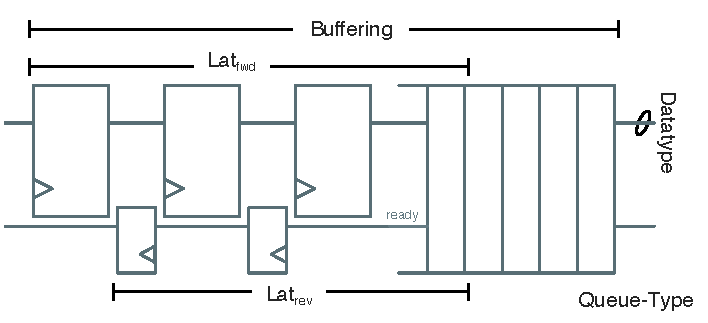
\includegraphics[width=\columnwidth]{figures/queue-channel.pdf}
        \caption{A queue type channel with its four characteristic parameters.}
        % graffle2pdf -c queue midas-graphics/graffle/channel-types.graffle figures/queue-channel.pdf
        \label{fig:queue-channel}
    \end{subfigure}
    \begin{subfigure}[t]{0.34\textwidth}
        \captionsetup{margin=0.25cm}
        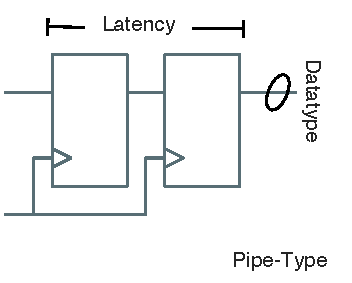
\includegraphics[width=\columnwidth]{figures/pipe-channel.pdf}
        \caption{A pipe-type channel. Setting latency to zero models a wire.}
        % graffle2pdf -c pipe midas-graphics/graffle/channel-types.graffle figures/pipe-channel.pdf
        \label{fig:pipe-channel}
    \end{subfigure}
    \centering
    \caption{Two types of channels used in a channel-bootstrapped formalism.}
\end{figure}


Addressing this, APort Networks~\cite{APortNetworks} was designed to support
finer-grained LPs that are coupled with register stages in the target. In their
paper, Pelleaur et al. use a processor pipeline as a motivating example and
divide different pipeline stages into seperate LPs. Later versions of the RAMP
architecture introduced the same sort of channel, which we call a \emph{pipe}
channel, shown in Figure~\ref{fig:pipe-channel}.  Pipe channels are defined by
a single parameter $l$, corresponding to their latency. Assuming the underlying
registers they model are not reset explicitly a using target signal, but are
instead initialized at time 0 to some statically known value, pipe channels
provide $l$ initial messages before they must stall for an input message.

Neither formalism appears to give any treatment to modeling a target-driven reset in
channels, as they both rely on time-zero intialization to effectively
"reset" target state.  We note that if these underlying state elements are
synchronously reset, the channels with $l >= 1$ may provide no more than 1
initial message, as future messages may causually depend on a reset
message\footnote{We further note that neither of these formalisms was designed
to support asynchronously reset as all-events are synchronous to an implicit
clock. At a first blush, however, asynchronous reset mandates that that even
the first message emitted by a pipe-channel with $l > 0$ would depend causually
on reset at time 0.}. A pipe-type channel with $l = 0$, is a degenerate LP that models a wire between the producer and consumer LP, coupling them combinationally.
It models no target state and merely relays messages from producer to consumer.

In both formalisms, units model a single target cycle of execution by dequeuing an input message
from each of its input ports, and enqueing a new output message into each of
it's output ports. The simplest unit implementation, and the one perscribed by
APort Networks, waits for all input messages to arrive and all of it's output
ports to be ready to accept to messages, before it may \emph{fire}. Then the
unit computes its state updates and simulateously enqueues a single output
message into each output port, and dequeues a message from each input port.
Figure~\ref{fig:adder-example} demonstrates the execution of a single target cycle in a channel-bootstrapped formalism.

\begin{figure}
    \centering
    \begin{subfigure}[t]{0.49\textwidth}
        \captionsetup{margin=0.25cm}
        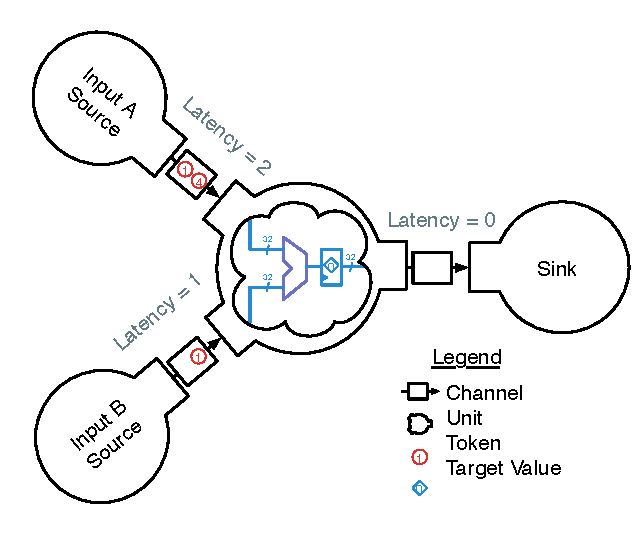
\includegraphics[width=\columnwidth]{figures/adder-example1.pdf}
        \caption{Initial state of the graph.}
        % graffle2pdf -c initial-state midas-graphics/graffle/adder-example.graffle figures/adder-example1.pdf
    \end{subfigure}
    \begin{subfigure}[t]{0.49\textwidth}
        \captionsetup{margin=0.25cm}
        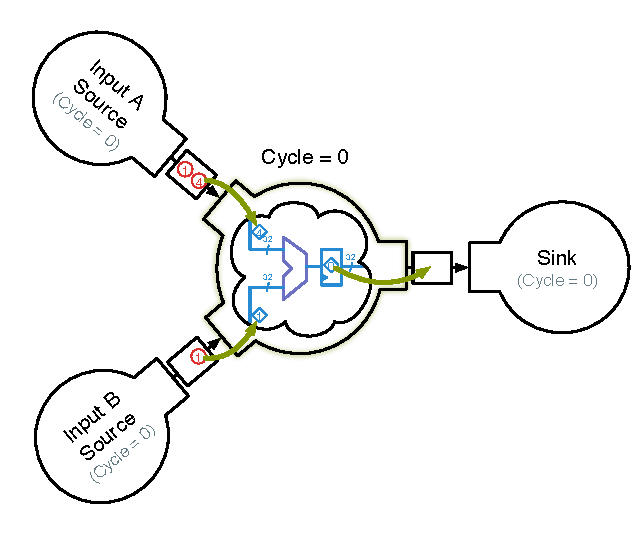
\includegraphics[width=\columnwidth]{figures/adder-example2.pdf}
        \caption{With all input tokens available, the unit fires and advances to cycle 1.}
        % graffle2pdf -c tfire-cycle0 midas-graphics/graffle/adder-example.graffle figures/adder-example2.pdf
    \end{subfigure}
    \begin{subfigure}[t]{0.49\textwidth}
        \captionsetup{margin=0.25cm}
        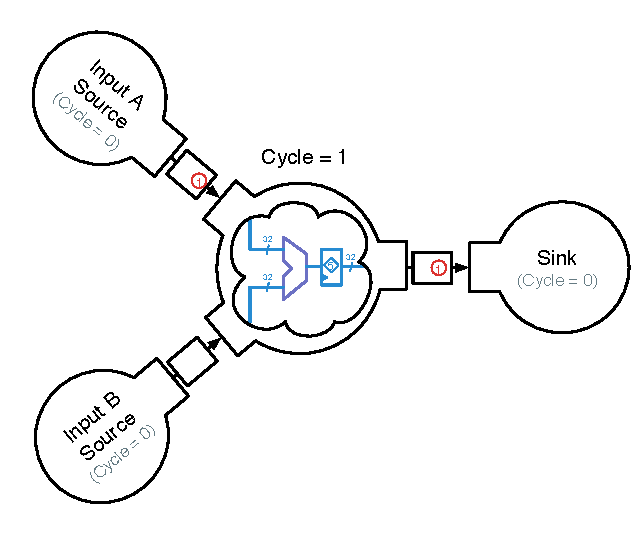
\includegraphics[width=\columnwidth]{figures/adder-example3.pdf}
        \caption{The state of the graph after firing. The unit is stalled on the arrival of a B-input token.}
        % graffle2pdf -c cycle1 midas-graphics/graffle/adder-example.graffle figures/adder-example3.pdf
    \end{subfigure}
    \begin{subfigure}[t]{0.49\textwidth}
        \captionsetup{margin=0.25cm}
        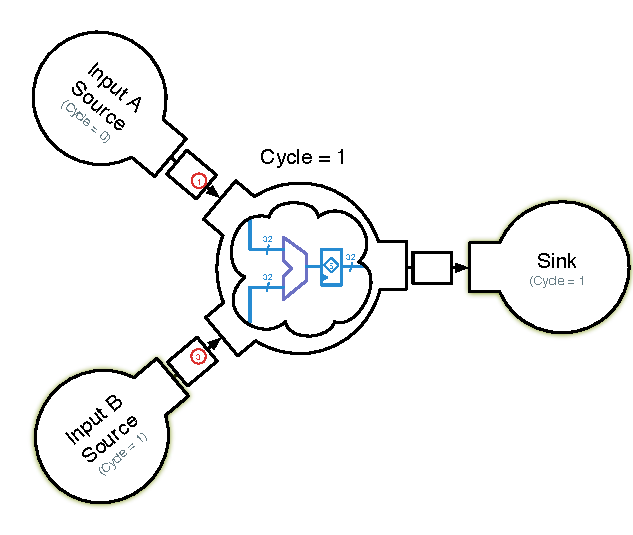
\includegraphics[width=\columnwidth]{figures/adder-example4.pdf}
        \caption{Input B source fires, producing the needed token.}
        % graffle2pdf -c inputb-fires midas-graphics/graffle/adder-example.graffle figures/adder-example4.pdf
    \end{subfigure}
    \begin{subfigure}[t]{0.49\textwidth}
        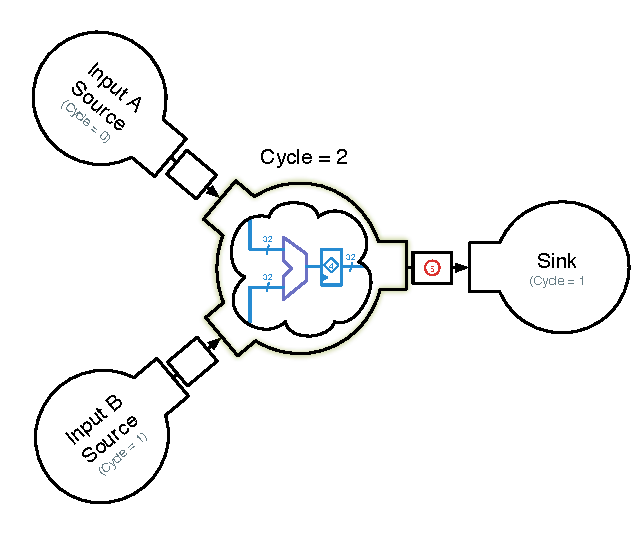
\includegraphics[width=\columnwidth]{figures/adder-example5.pdf}
        \caption{The state of the graph after two firings of the unit.}
        % graffle2pdf -c cycle2 midas-graphics/graffle/adder-example.graffle figures/adder-example5.pdf
    \end{subfigure}
    \centering
    \vspace{-0.25in}
    \caption{A 32-bit adder model and environment simulating a single cycle of target time.}
    \label{fig:adder-example}
\end{figure}

If the simulation designer uses exclusively, non-wire-type channels both
formalisms are free of deadlock, as there exists no unit whose output at cycle
$t$ depends on the output of another unit also at cycle $t$\footnote{From a
conservative PDES persective, every LP has a non-zero lookahead, and given that
every LP sends messages at every timestamp (obviating the need for null
messages), deadlock is avoided by construction}. In these simulators, all units
can excute cycle $t$ concurrently, which assuming no other sources of delay,
permits the simulator to run at unity FMR.  However, as with latency-insensitive boundaries, it is not always possible to define LP
at registered boundaries.  The use of wire-type channels, (i.e. combinational
coupling between LPs) that introduces two principle challenges: at best, it
increases simulator FMR, and at worst, it may introduce time-zero simulation
deadlock. To illustrate each of these effects, in Figure~\ref{fig:channel-deadlock} we consider a
latency-insensitive interface between two units implemented three different ways: with a queue-type
channel, with one pipe and one wire-type channel, and with two wire-type channels.

\begin{figure}
    \centering
    \begin{subfigure}[t]{0.49\textwidth}
        \captionsetup{margin=0.25cm}
        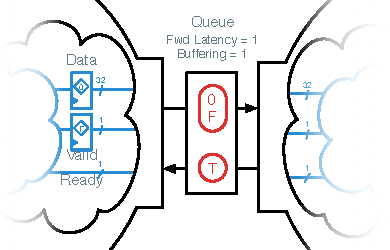
\includegraphics[width=\columnwidth]{figures/li-queue-channel-manual.pdf}
        \caption{A RAMP-style queue-type channel. This allows both models to
        fire simultaenously, but may only be used if it is acceptable to model
        a target queue in the channel.}
        %  -c queue midas-graphics/graffle/deadlock.graffle figures/li-queue-channel.pdf
    \end{subfigure}
    \begin{subfigure}[t]{0.49\textwidth}
        \captionsetup{margin=0.25cm}
        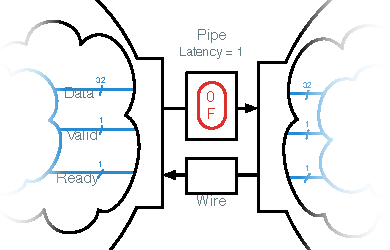
\includegraphics[width=\columnwidth]{figures/li-pipe-channel-manual.pdf}
        \caption{One pipe-type channel, and one-wire type channel carrying the backpressure. This leads $FMR >= 2$, with the consumer unit
        firing first to produce a backpressure token that is subsequently consumed by the producer unit.}
        %  -c pipe midas-graphics/graffle/deadlock.graffle figures/li-pipe-channel.pdf
    \end{subfigure}
    \begin{subfigure}[t]{0.49\textwidth}
        \captionsetup{margin=0.25cm}
        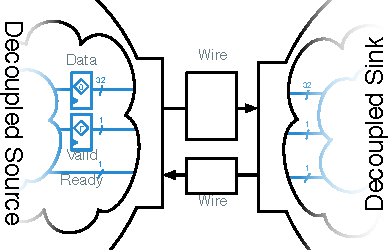
\includegraphics[width=\columnwidth]{figures/li-wire-channel-manual.pdf}
        \caption{Two-wire type channels. This deadlocks an APort Network, as neither producer nor consumer unit can fire
        before the other.}
        % -c wire midas-graphics/graffle/deadlock.graffle figures/li-wire-channel.pdf
    \end{subfigure}
    \centering
    \vspace{-0.25in}
    \caption{Three potential channel modelling decisions for a latency insensitive interface between two units.}
    \label{fig:channel-deadlock}
\end{figure}

In the absence of deadlock, wire-type channels tend to increase FMR as in
general a combinational path that spans $N$, units will take $N$ cycles to
execute. Note that other channels connecting these units tends to prevent
pipelining multiple cycles of target execution (i.e., this latency cannot be
overlapped, with the simulation of younger target cycles).

Deadlock is the more pressing challenge. Wire-type channels remove the
aforementioned property that all LPs have non-zero lookahead.  Here there are
two situations that may emerge. If the target itself has a combinational loop,
the behavior of the physical system is itself undefined, and simulation
deadlock is unavoidable~\footnote{We note it is possible to have "false"
combinational loops but many tools reject these patterns, and so it's not
unreasonable to ban them in these simulators as well.}. As a matter of
practise, hardware designers know to avoid combinational loops. The second
challenge arises from poor LP implementation, such as the unit perscribed by
APort Networks, that attempts to enqueue and dequeue multiple messages
atomically. Mandating this implementation has the effect of introducing a
dependency between all output messages on all input messages, even though there
they may be no combinational path between many of these outputs and inputs in
the underlying target. Given its definition of a unit, APort Networks do not
give the correct set of constraints to avoid deadlock as a graph that contains
a cycle of wire-type channels -- that do not represent a combinational loop in
the target -- deadlocks at time zero.


\subsection{Latency-Insensitive Bounded-Dataflow Networks}

Unlike channel bootstrapped formalisms, LI-BDNs avoid deadlock by imposing
different constraints on the implementation of LPs based on the underlying
hardware they model, and remove the need for specialized channels to bootstrap
simulation. Since connections between LPs always represent wire-like
connectivity, LI-BDNs impose no contraints on how the target
is divided into LPs. LI-BDNs were originally developed as a more flexible abstraction for building
latency-sensitive designs that preserve the RTL timing of a synchronous circuit, extending
the work of Carloni et al., in the Theory of Latency Insensitive Design, however the authors identify that this problem is analogous
to constructing an ITDC simulator from synchronous ASIC RTL.

In the terms of the paper, what we have loosely referred to as a synchronous
block of RTL thus far is defined synchronous sequential machine~(SSM). Vijayaraghavan et
al.\cite{LIBDN} formally define an SSM:

\begin{widequote}
An SSM is a network of combinational operators or gates
such as AND, OR, NOT, and state elements such as registers,
provided the network does not contain any cycles which has
only combinational elements.
\end{widequote}

Missing from this definition is any treatment of multiple clock domains, different
types of state elements, asynchronous set or reset.  Inherent to the name
``synchronous'', Vijayaraghavan et al. forbid their existence -- in an SSM
\emph{all} state updates occur simultaenously. While this limits the
applicability of their approach, much of a modern SoC, such as the islands of a
GALS-based design, locally meets this definition.  With it's simple
state-update semantics, any SSM can be easily converted into a \emph{patient}
SSM; the equivalent circuit whose state update can be controlled with the assertion of a global enable signal.
One way this conversion can be achieved, proposed by the authors, is by
disabling register updates and masking off RAM write-enables when this control
signal is unset. Alternatively, we note that the SSM may be clock gated.

With an SSM defined, we can now define an LI-BDN, and how they can be used to implement any
SSM in an latency-insensitive manner. An LI-BDN is a dataflow network of latency-insensitive nodes whose
edges represent FIFO communication channels with non-zero, but finite (hence,
bounded) capacity. The latency-insensitive nodes of the graph are
referred to as \emph{Primitive LI-BDNs}~(in PDES terms, these are LPs), which is to say, they 
are not themselves subgraphs of more than one node. A
LI-BDN is said to \emph{implement} an SSM, if it \emph{partially implements}
the SSM, and is deadlock free. In the terms of a hardware engineer, partial implementation~(PI) implies that
the message trace of outputs from the ports of the LI-BDN "matches" the
per-cycle trace of outputs from the SSM. Vijayaraghavan et al.\cite{LIBDN}
formally define PI:

\begin{widequote}
A BDN $R$ partially implements an SSM $S$ iff
\begin{enumerate}
\item There is a bijective mapping between the inputs of $S$ and
[the input tokens of] $R$, and a bijective mapping between the outputs of $S$ and
[the output tokens of] $R$.
\item The output histories of $S$ and $R$ match whenever the
input histories match, i.e.,
\begin{align*}
\forall n &> 0\\
&\text{$I(k)$ for $S$ and $R$ matches $(1 \leq k \leq n)$}\\
\Rightarrow &\text{$O(j)$ for $S$ and $R$ matches $(1 \leq j \leq n)$}
\end{align*}
\end{enumerate}
\end{widequote}

All SSMs have infinitely many possible partial implementations~\footnote{For
instance, one can take any existing partial implementation, and introduce an
extra cycle of delay on any of its outputs. As we'll show later, since it's
always possible to produce an LI-BDN from any SSM, it follows by induction that are infinitely many partial implementations
for any SSM.}, though some implementations deadlock when composed into larger graphs.
Consider the unit implementation perscribed by APort Networks. It is a valid partial implementation of
the source RTL, however, it cannot \emph{implement} a larger SSM when it is composed 
with other liked-styled implementations without the use of non-wire-type channels (which themselves
are a special form of LP that remove zero-cycle loops between units).
Conversly, LI-BDNs garauntee deadlock freedom by adhering to two additional properties.
The first is \emph{No Extraenous Depedencies}~(NED) which defines when an LP is obligated to enqueue output messages. Vijayaraghavan et al.\cite{LIBDN} formally define NED:

\begin{widequote}
A primitive BDN has the NED property if all output FIFOs have been enqueued at least $n-1$ times,
and for each output $O_i$, all the FIFOs for the inputs in $\emph{CombinationallyConnected}(O_i)$
are enqueued $n$ times, and all other input FIFOs are enqueued at least $n-1$ times, then $O_i$ FIFO
must eventually be enqueued $n$ times.
\end{widequote}\label{def:ned}

One intuitive explanation of NED is that it exploits the same observation that
permits a pipe-type channel to send output messages before receiving any input
messages: any output driven only by state in the LP (i.e., outputs not
combinationally coupled to an input) can enqueue an output messages for cycle
$t$ before receiving any input messages for cycle $t$. NED broadens this to apply to logic cones fed not just by state
elements but those that depend only on a subset of the LP's inputs.

The second property an LI-BDN must satisfy is the \emph{self-cleaning}~(SC) property. SC 
defines when an LP is obligated to dequeue input tokens. Vijayaraghavan et al.\cite{LIBDN} formally define SC:

\begin{widequote}
A primitive BDN has the SC property, if when all the
outputs are enqueued $n$ times, all the input FIFOs must
[eventually]\footnote{Clarified in~\cite{LIBDNMasters}.} be dequeued $n$ times, assuming an infinite source for each
input.
\end{widequote}\label{def:sc}

While the nodes of an APort Network do not always satisfy NED, they do satisfy
SC. At it's heart, SC provides an assurance that LPs drain their input FIFOs,
allowing those FIFOs remain bounded. We note that if an LP fails to satisfy
SC, it will likely fail to partially implement its SSM unless its outputs are
completely independent of the inputs from which it is failing to dequeue. In
this case having unbounded FIFOs would suffice to prevent deadlock.

Of particular concern to this dissertation is a method through which an SSM can
be converted into a primitive LI-BDN.  Vijayaraghavan et al. describe a means that uses
a wrapper module around the patient SSM based on it's combinational
depedencies. The SSM is treated as a black box otherwise. The wrapper circuit,
for a single output, is shown in \ref{figure}. This method is highly amenable
to automation with a FAME compiler, as it requires only the ability analyze
combinational depedencies in the underlying SSM.

\section{The MIDAS Compiler \& Simulator Microarchitecture}

As we first introduce in Section~\ref{sec:midas-intro} mentioned previously,
MIDAS was our first attempt at building a RAMP compiler. Here we describe the
version of MIDAS released with FireSim 1.5.0, which differs modestly from earlier iterations 
described in the CARRV paper~\cite{MIDAS} and Donggyu Kim's dissertation~\cite{DGKDissertation}.

MIDAS generates ITDC simulators directly from ASIC RTL; these simulators that
implement a channel-bootstrapped formalism, with all target graphs having a
star topology. We show an example graph for a Rocket-Chip-based system, the
most commonly used target generator in MIDAS, in Figure~\ref{fig:rocket-target-graph}
"hub" unit is transformed from ASIC RTL elaborated by a user-provided Chisel
generator. This RTL does not represent a
closed system -- it exposes I/O interfaces that must be tied to units that model those
devices. These units are called \emph{endpoints} and form satelite nodes in the graph.
MIDAS-generated simulators are designed to run on hybrid CPU-FPGA hosts
with the expectation being that certain tightly coupled endpoints, such a DRAM
timing models, will be written in RTL and hosted on the FPGA, while other higher
latency, less performance critical ones, such UART and block device models, can
be written in software hosted on the CPU. We refer to the CPU-hosted componenet
of the simulator as the \emph{driver}. To avoid deadlock and provide good
simulation FMR, MIDAS injects queue-type channels (to model a 2-deep,
fully-decoupled FIFO) on all decoupled interfaces, and 1-cycle-latency
pipe-type channels. Assuming units do not stall internally, MIDAS-generated
simulators can run at unity FMR. We show an example simulator mapped to an EC2 F1 host in Figure~\ref{fig:mapped-simulator-f1}.

\begin{figure}
    \centering
    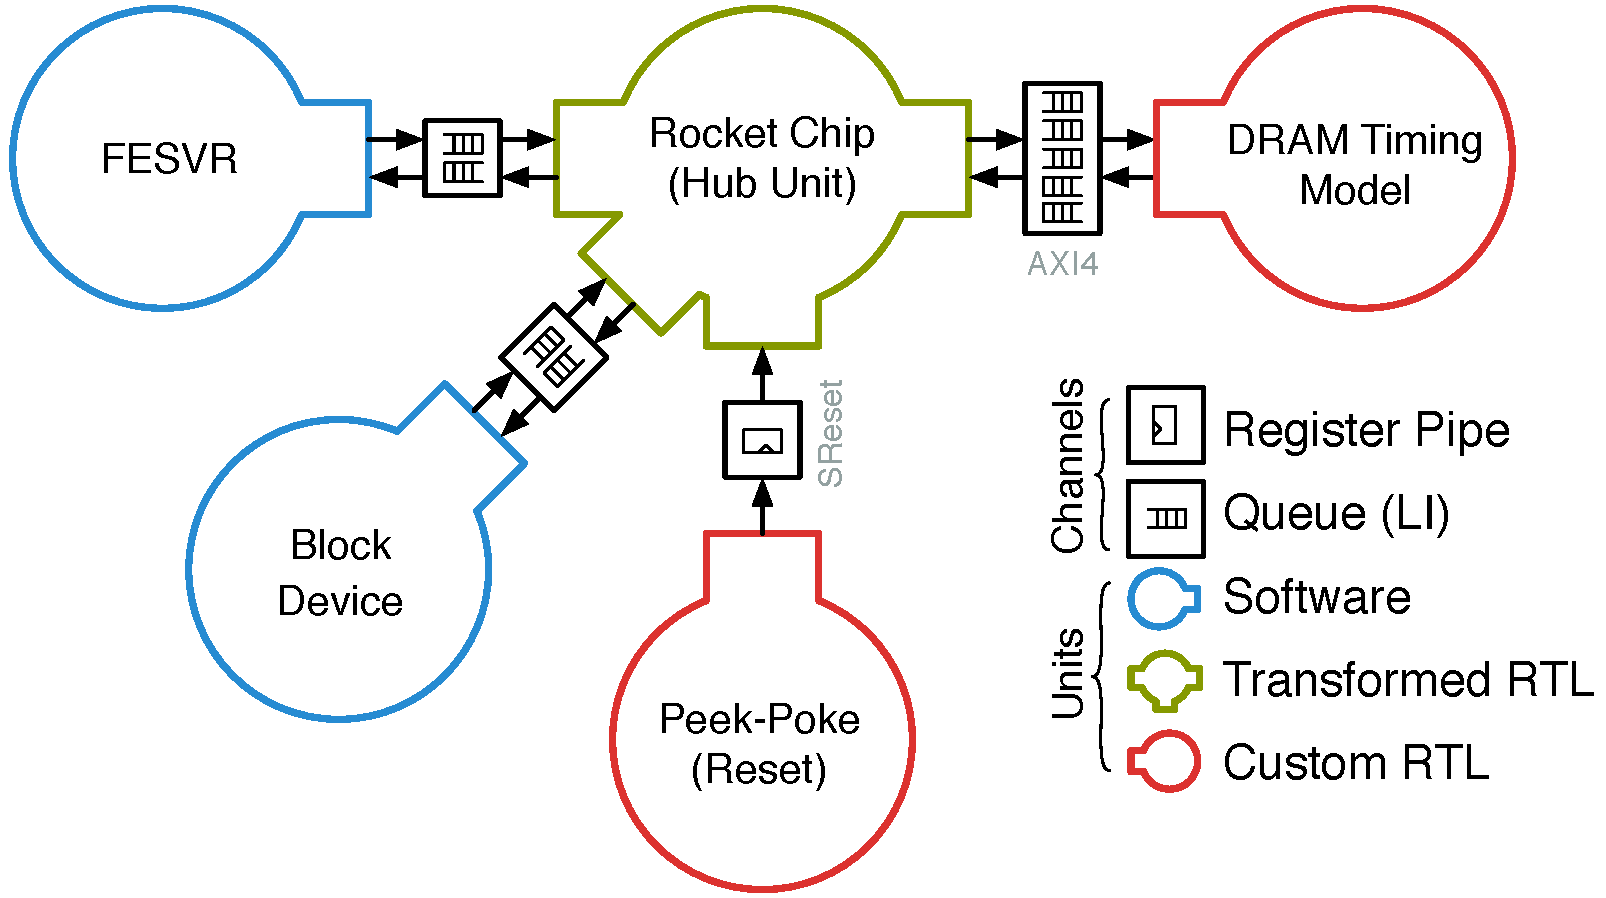
\includegraphics[width=0.9\textwidth]{figures/rocket-target-graph.pdf}
    % graffle2pdf -c rocket-target-graph midas-graphics/graffle/masters-target.graffle figures/rocket-target-graph.pdf
    \caption{The graph of a typical Rocket-Chip-derived system.}
    \label{fig:rocket-target-graph}
\end{figure}

\begin{figure}
    \centering
    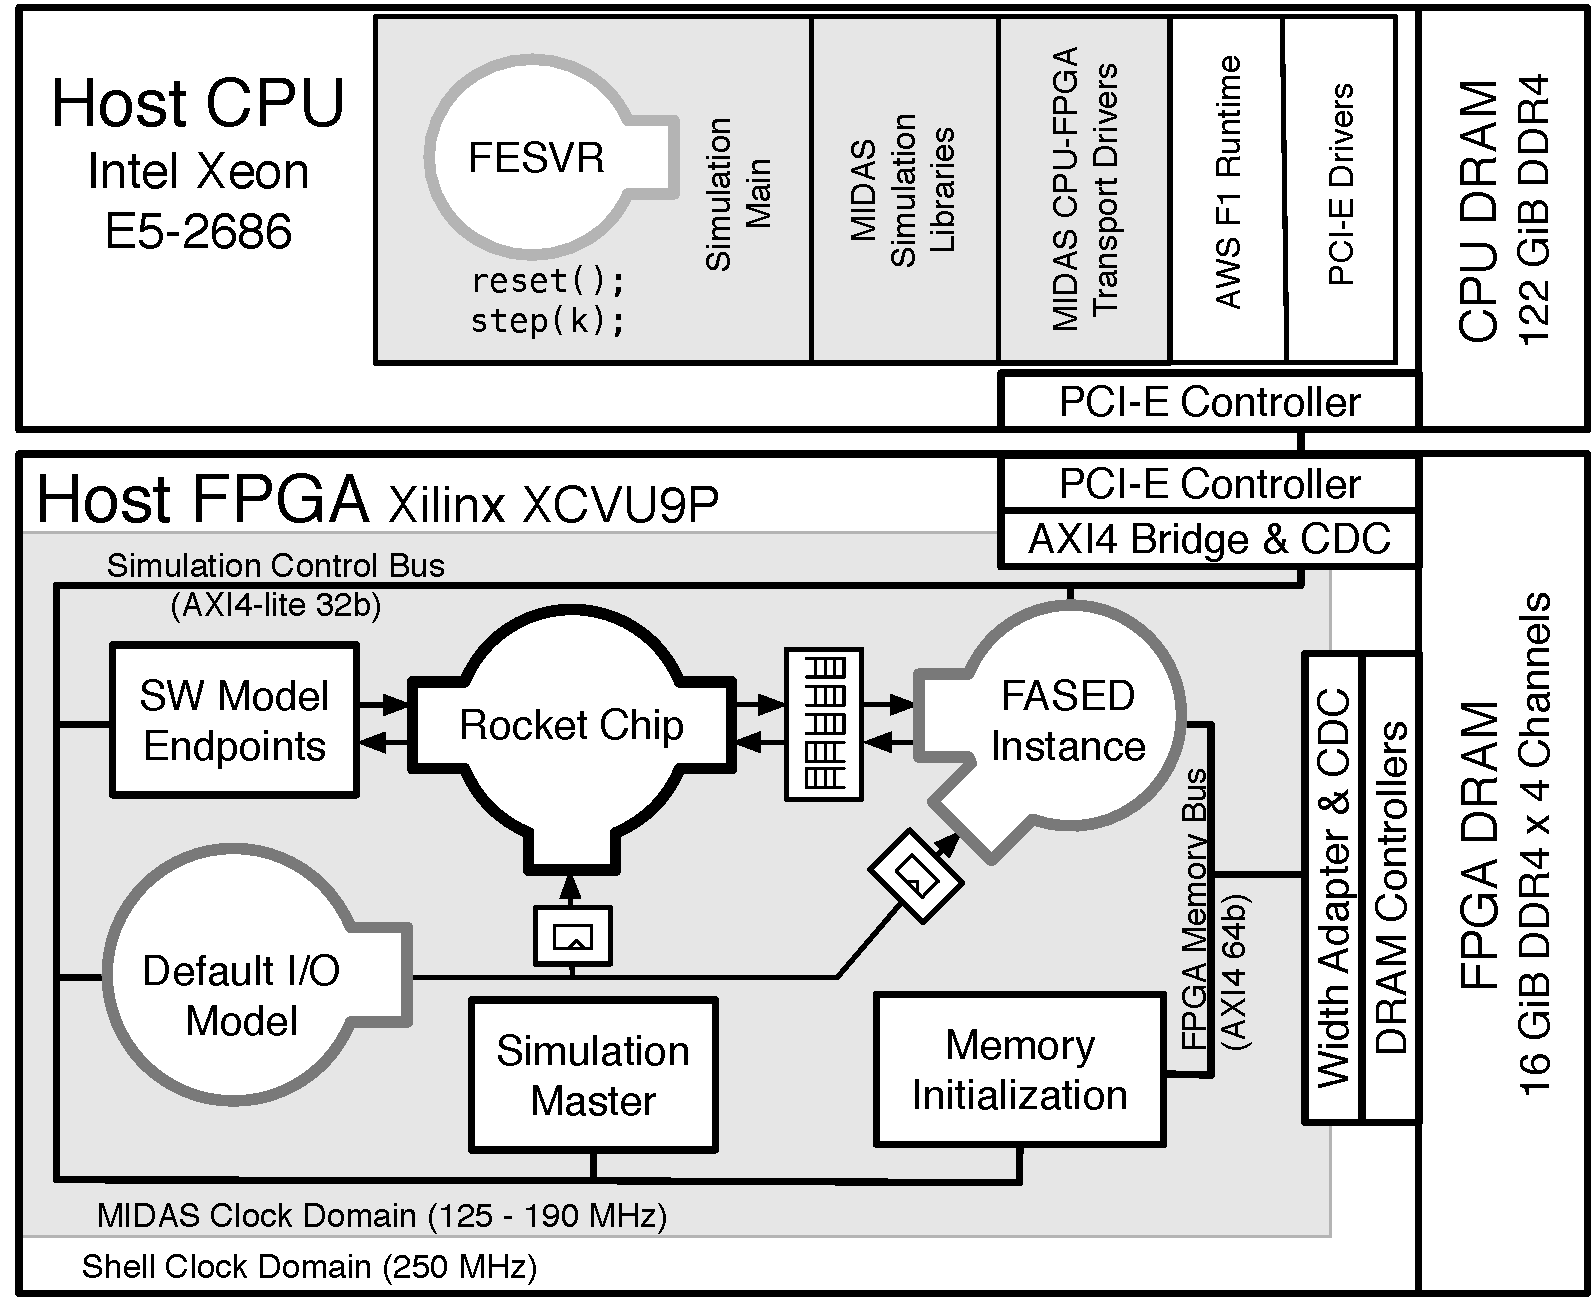
\includegraphics[width=0.9\textwidth]{figures/mapped-simulator-f1.pdf}
    % graffle2pdf -c f1 midas-graphics/graffle/mapped-simulator.graffle figures/mapped-simulator-f1.pdf
    \caption{An example simulator mapped to and EC2 F1 host.}
    \label{fig:mapped-simulator-f1}
\end{figure}


\subsection{Endpoint Units}

Topological position aside, endpoint units differ from the hub in that they are not transformed from ASIC
RTL and instead are written by hand, and thus, not exact models of the desired target system.
Endpoints consist of an \emph{endpoint module}, which resides on the FPGA and drives the channels bound to the hub unit, and an
\emph{endpoint driver}, which is linked into the main simulation driver and hosted on a CPU.
Even the purest "CPU-hosted" units require an endpoint driver that
implements transport for token streams moving on and off the
FPGA\footnote{FireSim stitched together larger targets by adding software units
to represent parts of the network. These were hosted purely on a CPU, often
with no FPGA attached.} Similarly, FPGA-hosted models tend to have a driver
that is reponsible for configuring the FPGA-hosted piece of the unit, and for
polling FPGA-hosted instrumentation.

Endpoints can leverage three types of host resources:

\begin{enumerate}
\item CPU-mastered MMIO. Here, modules expose 32-bit registers that can be
    written to and read from the driver. This is typically used to expose
    configuration  parameters that the driver initializes before simulation
    commences, and to expose instrumentation that can be polled during
    simulation. Generally, MMIO cannot provide enough bandwidth to support transporting token streams,
    for low-bandwidth, loosely coupled endpoint it can also be used to pass transaction-level messages.
    The endpoints for UART and the FireSim block device do this.

\item CPU-mastered DMA. To support moving complete token streams, endpoints can
    bind to CPU-mastered DMA. Here endpoint modules expose hardware FIFOs to the DMA bus to which the driver
    can make bulk (up to 4192KB) reads and writes. If the endpoint is not closely coupled
    to the hub, token transport can be overlapped with simulator execution: the NIC endpoint relies on this
    provide good FMR in networked simulations~\cite{FireSim}. CPU-mastered DMA is also used 
    to drain token streams from instrumentation endpoints. Since these endpoints do not drive
    tokens back to the hub, it is only necessary to provide sufficient DMA read-bandwidth to achieve good FMR.
    Examples of this include the synthesized printf endpoint and the TracerV
    RISC-V instruction trace collection endpoint.

\item FPGA DRAM. Some units require more local storage than FPGA fabric can
    provide, but cannot afford the round trip latency of using CPU memory or
    disk. MIDAS provides a simple means to let endpoints drive the FPGA
    DRAM memory system.  MIDAS's memory timing models, both those described
    in the CARRV publication~\cite{Midas} and later by FASED~\cite{FASED},
    use FPGA DRAM as a backing store for a timing model that's implemented
    in FPGA fabric.
\end{enumerate}

Endpoint drivers interact with their associated module using four methods
exposed by the main simulation driver: \texttt{simif::read} and
\text{simif::write} drive CPU-mastered MMIO; \texttt{simif::pull} and
\texttt{simif::push} are used to drive CPU-mastered DMA.

\subsection{Simulation Driver}

The simulation driver is written in C++ and instantiates an endpoint driver class for each endpoint
in the system. Once the FPGA has been flashed, the driver can be launched.
Simulation proceeds in three phases:

\begin{enumerate}
    \item Initialization. This provides a window for endpoint drivers to do DMA
        and MMIO before the simulation commences.  Here the driver optionally
        zeros-out or intializes FPGA DRAM, before calling each endpoint
        driver's \texttt{init} method, which sets up configuration registers on
        the FPGA that may control timing parameters or instrumentation modes.

    \item Execution. Here the driver invokes each endpoint's \texttt{tick}
        method in a tight loop, in round-robin order.  Drivers issue MMIO and
        DMA requests attempting to make forward progress without blocking.

    \item Teardown. Simulation ends once any endpoint driver calls for
        termination. The driver calls each endpoint's \texttt{finish} method,
        which gives the endpoint a final opportunity to do FPGA DMA and MMIO. This
        typically includes reading final FPGA-hosted intrumentation values and commiting simulation output to disk.
\end{enumerate}


\subsection{Time Control}
After FPGA programming and reset, channels are ready to produce initial tokens and thus units are free
to begin executing. Generally, endpoints that require
configuration wait for an MMIO register to be set during the driver's
intialization phase before acting on token streams. In the absence of
user-provided endpoints, MIDAS prevents the hub model from free-running by
mandating that all target designs have a synchronous reset that is driven
by a special \emph{peek-poke} endpoint. The peek-poke endpoint ties off all
unnconnected I/O on the target to memory-mapped registers
that can be driven to specific constants during initialization, or
periodically changed during simulation. The driver can then "step" the hub
by controlling the emission of reset tokens by the peek-poke endpoint.
Unlike for other endpoints, channels between the peek-poke endpoint and hub
are the only channels that are wire-type by default: enqueuing a $k$ reset
tokens permits the hub to advance no further than cycle $k$.

During simulation teardown, the simulator estimates the number of cycles simulated by
reporting the number of reset tokens enqueued by the endpoint. In practise,
the hub may not have drained all tokens in the reset channel (it is in the
past relative to the peek-poke endpoint), and additionally, other endpoints
connected to the hub may be relatively more or less advanced in simulation
time due to the distributed nature of the simulator.

\subsection{Using MIDAS: Generator Side Integration}

MIDAS functions by providing an alternate generation flow for a chisel
generator.  In their Scala application, the user lazily instantiates their
module class and calls out to chisel elaboration as they normally would.
This produces a FIRRTL circuit and annotations for what will become the hub
model.  Typically the lifetime of a chisel module class ends after
elaboration, however the lazy reference to the class allows the user to
extract the Scala types and names of the I/O interfaces of the top-level
module after elaboration. This is critical as MIDAS determines how to bind
endpoints to the hub unit by querying a user-provided map of Chisel type to
endpoint module for each of the extracted I/O interfaces. Finally, the user
invokes the compiler, passing the FIRRTL circuit and annotations, the
extracted I/O list, separate lists of FIRRTL transforms to run on the
elaborated RTL and then the complete simulator, and an implicit parameters
instance which provides the aforementioned map and set switches to control
various stages of the compiler.

\subsection{MIDAS Compiler Flow}

\begin{figure}
    \centering
    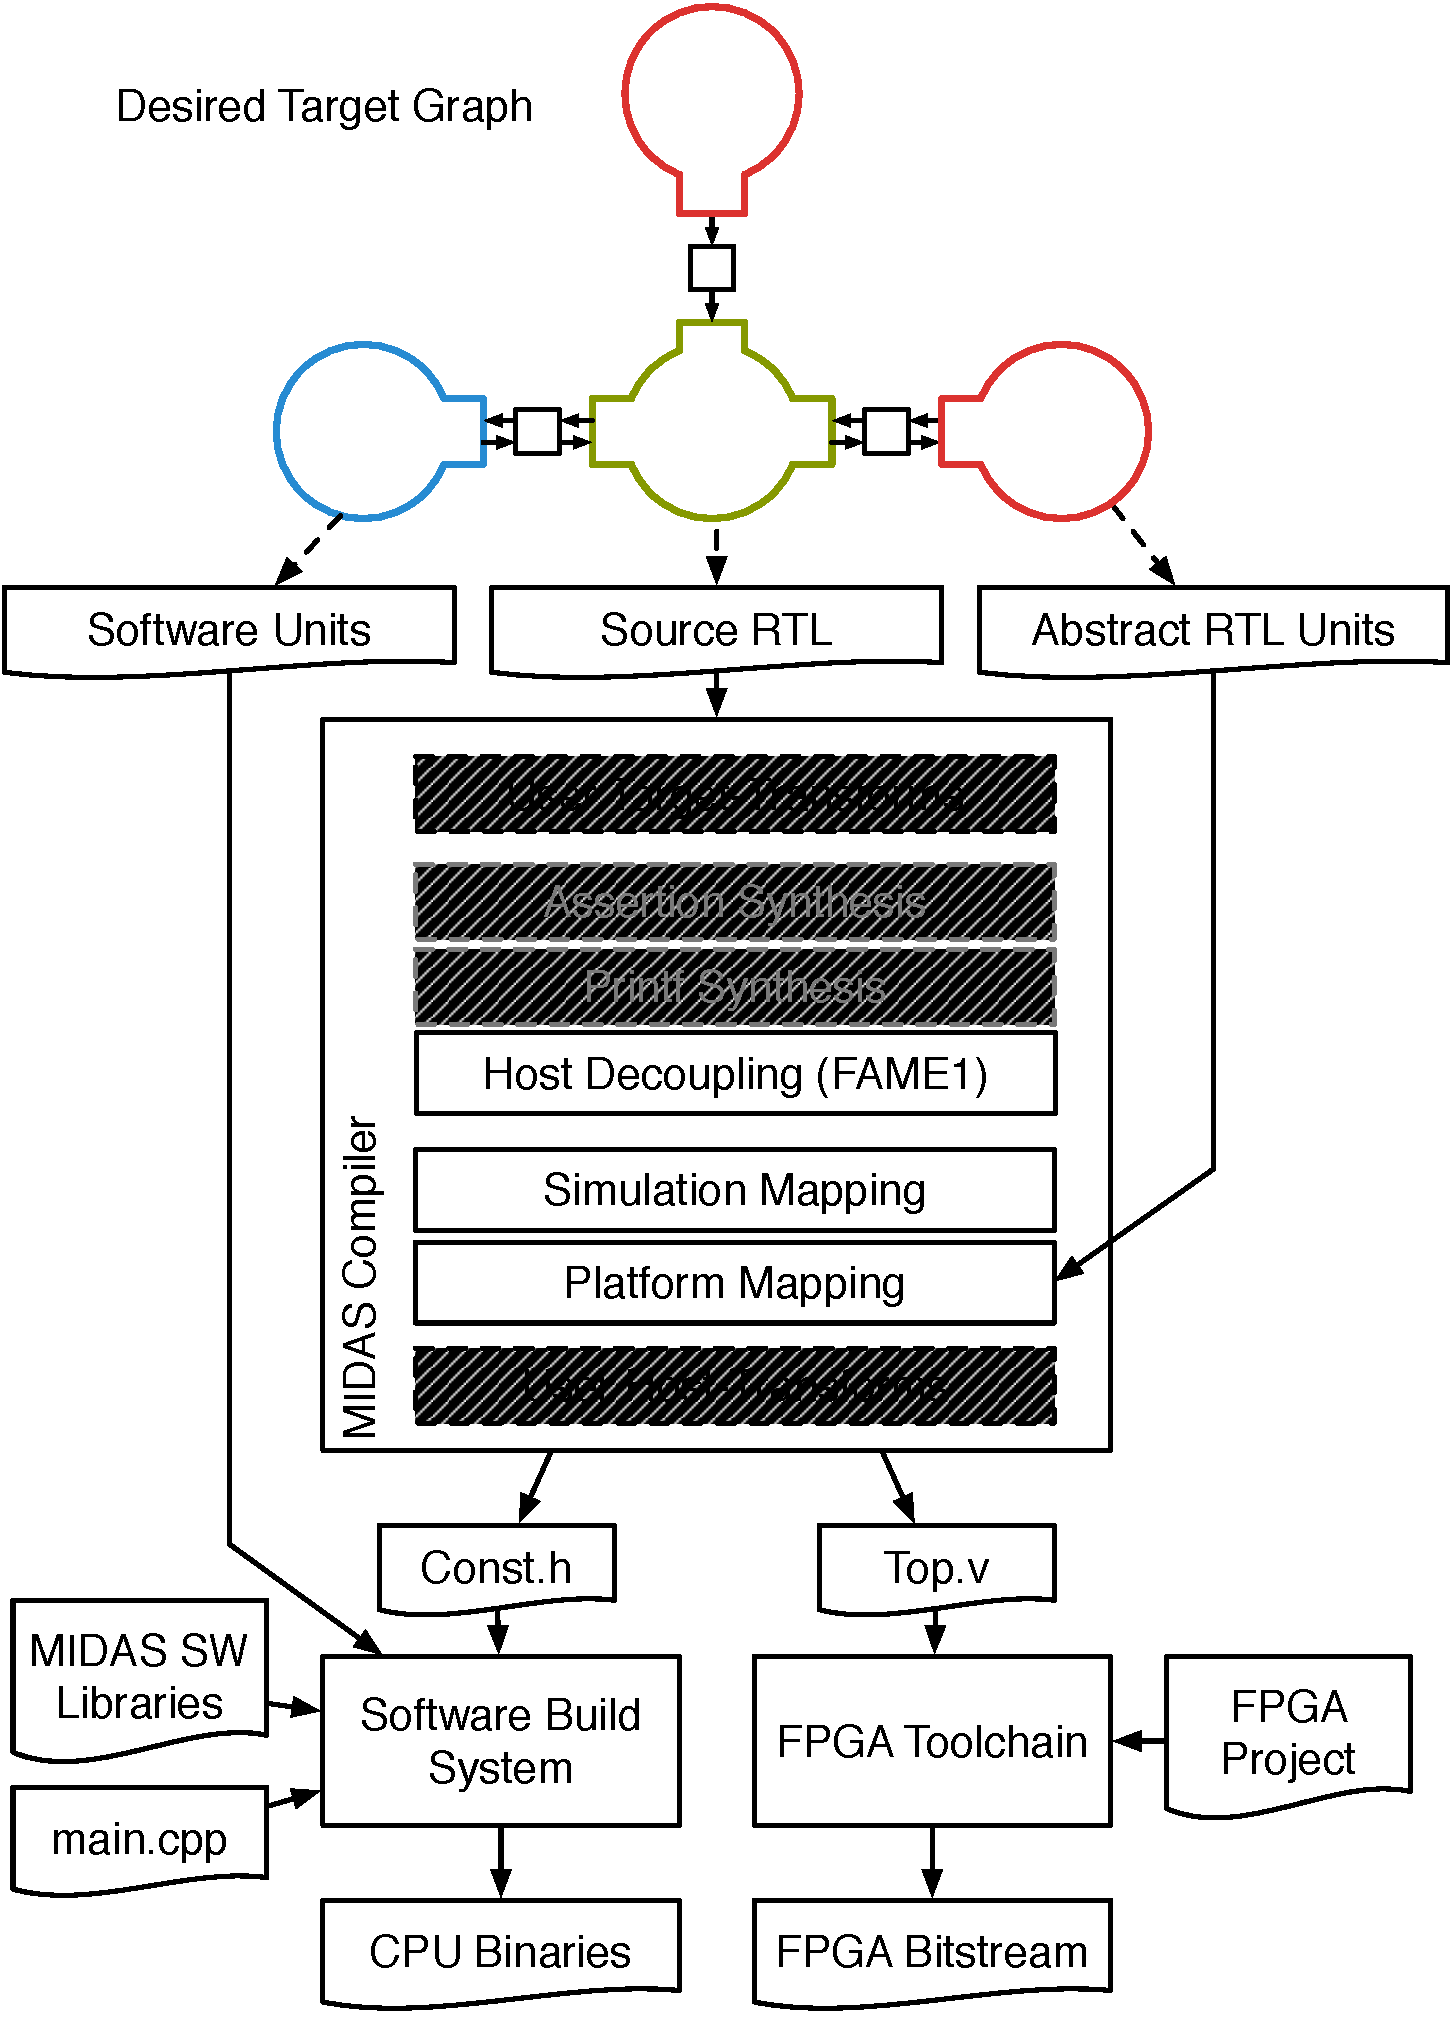
\includegraphics[width=0.9\textwidth]{figures/midas-flow.pdf}
    % graffle2pdf -c midas-flow midas-graphics/graffle/toolchain.graffle figures/midas-flow.pdf
    \caption{The end-to-end flow of a MIDAS compilation.}
    \label{fig:midas-flow}
\end{figure}

    We show the flow the MIDAS compiler in Figure~\ref{fig:midas-flow}.

    Before running core transformations, MIDAS schedules user-provided target transforms.
    In FireSim, dedicated passes to remove unsupported verilog black-boxes and
    replace asynchronously reset registers synchronously reset ones.

    Next MIDAS runs instrumentation transformations, including printf synthesis
    and assertion synthesis~(these were initially presented in DESSERT~\cite{DESSERT}), if they have been requested by the user. These
    transformations "synthesize" \texttt{printf} and \texttt{stop} FIRRTL IR
    nodes by replacing them with a connections to new top-level outputs. Stops are
    replaced with a boolean that is asserted on cycles the stop condition is asserted. Similarly, printfs are replaced with an aggregate that contains
    the arguments for the printf's format string and an enable indicating the
    printf would trigger on that cycle. Like the other I/O interfaces, these new outputs will be bound to a single asssertion
    and printf endpoint later in the compiler.

    Now MIDAS runs its FAME-1 transform, transforming the RTL (an SSM) into a
    unit.  MIDAS converts the SSM into a patient SSM by injecting clock-enables
    on all registers (this introduces a 2:1 mux on register inputs) and by
    masking FIRRTL memory write enables. The transform divides and maps the
    SSM's I/Os into message ports by recursing through their corresponding Chisel types.
    Decoupled interfaces~(latency-insensitivity interfaces that use a ready-valid
    handshake) are split into a forward and reverse port, all other
    interface types are given a seperate port per leaf-element.  With the I/Os
    mapped into unit ports, the transform drives \texttt{fire} with the
    conjuction of all inputs' valid and all outputs ports' ready. The resulting
    unit is a direct implementation of an APort Network node.

    To complete the simulator, MIDAS then wraps the hub unit with two layers of Chisel-generated modules.
    In \emph{Simulation Mapping}, MIDAS again recursively walks the chisel-types of the I/O, this time
    to generate the channel implementations.
    Wire and pipe-type channels are implemented using a queue whose
    payload is the underlying hardware type of the target interface. The endpoint and hub can decouple
    as many cycles as these queues are deep.  Queue-type channels use a more sophisticated implementation
    that drives forward and reverse token streams. The queue channel
    implementation allows endpoint and hub to decouple under more specific runtime conditions~(for example,
    while a queue is not full it can continue to accept forward tokens and produce reverse tokens on its the producer side
    of the queue.

    In \emph{Host Platform Mapping}, MIDAS recursively walks the chisel-types
    of the I/O a final time, here it attempts to find a provided endpiont for
    each type using the Endpoint Map. If the map is defined on that type, MIDAS
    instantiates the endpoint module, and connects its tokenized host port to the freshly
    generated channels. All remaining unbound interfaces are then bound to the
    peek poke endpoint. Once all endpoints have been elaborated, it binds their
    MMIO interfaces and DMA interfaces, if present, to the simulation control
    and DMA buses, respectively, using a $1:N$ AXI4 arbiter. Memory timing
    models have their host-memory interface driven to DRAM memory interfaces,
    this time through an $M+1:N$ AXI4 crossbar, where $M$ is the number of
    target memory models and $N$ is the number of host memory channels. The
    extra master port is driven by the loadmem unit, which bridges the
    simulation control bus and memory bus and gives the driver the means to
    read and write to FPGA DRAM. The parameters of the host platform,
    specifically the width of these buses, and the number of memory channels
    are defined in the user-provided parameters instance. At this point MIDAS,
    generates a C++ header with all of the driver-required metadata for the
    simulator. Each endpoint module emits a fragment which contains its allocated MMIO and
    DMA addresses, as well as additional constructor parameters required by its
    endpoint driver.

    In a final step before verilog emission, MIDAS schedules the user's
    \emph{host transforms}.  This permits modifying the simulator RTL to futher
    customize it for a host platform. In FireSim, the \texttt{AutoILA}
    transform is run here to plumb out annotated signals to a Xilinx Integrated
    Logic Analyzer (ILA), which is required in for EC2 F1 hosts due to
    restrictions in Amazon's compilation flow. Finally, the FIRRTL optimization passes are run
    and the simulator verilog is emitted, and the compiler terminates.

    At this point, the users links the generated header into the simulation
    main, and compiles the generated verilog into a FPGA shell project.
    FireSim's build system automates much of this, and provides an FPGA shell
    project for EC2 F1 FPGAs. FireSim's manager \texttt{buildafi} will batch
    out bitstream builds to remote hosts on EC2. Similary, its
    \texttt{infrasetup} process compiles the simulation driver, in addition to
    preforming the other required tasks to prepare for running a simulation
    including flashing the an FPGA.

\section{Reviewing MIDAS's Limitations}

    At the end of the previous chapter, we indentified two limitations with MIDAS 
    that we aimed to address in Golden Gate. The first was that it did little to optimize
    FPGA resource utilization, precluding the its use for systems of non-trivial scale. 
    We considered a few possibilities: leaning on the endpoint system and user modifications to the target RTL,
    specialized transformations to implement specific optimizations as modifications to the hub model. What was clear to us
    is that we had a few objectives.

    - Minimize user modification to the ASIC RTL timing
    - Make it possible to optimize blocks that may be combinationally coupled to some part of the hub.
    - Provide rigorous mechanism verify the resulting simulator


    Ultimately, it was clear that the next compiler needed a generalized
    mechanism to identify and perform optimizations. To make it easier to
    implement optimizations, Golden Gate uses the LI-BDN target formalism,
    removing the explicit need for channels. We acknowledge that forcing
    optimizations to apply only at registered boundaries between units -- a
    requirement of a channel-bootstrapped formalism -- would produce simulators
    with better FMR, this would add complexity to passes in the compiler and
    might make some optimizations infesible.  We also note that these sorts of
    optimizations not fundamentally precluded by LI-BDN: when an edge between
    two LPs is driven by an output port with no combinational dependency on an
    input, it may be possible to implement that edge using flow queue to save a
    cycle of transmission latency.

    Moving to an LI-BDN formalism resolves a number of other modeling
    challenges MIDAS users face.  Requiring that non-wire-channels be injected
    between endpoints and the hub unit was too restrictive in some cases where
    the user wishes to model a combinational path that propagated through the
    endpoint. Another challenge was defining the reset semantics of these
    stateful channels.  MIDAS relies on FPGA programming to properly initialize
    these channels, however they are not held in \emph{target-reset} during
    simulation: it is purely coincidental that the hub model does not
    spuriously enqueue target data into queue-type channels while parts of the
    hub are under target reset. For a time, MIDAS would broadcast target reset
    tokens to channels and endpoints, but too is fraught as resets driving
    registers in the hub maybe different from this special-cased global reset.
    Instead of requiring that user specify this reset for each channel, LI-BDN
    can sidestep these issues entire by removing the need for stateful
    channels, allowing the compiler to assume fewer things about target.

    Supporting realistic simulations of systems with multiple clock domains,
    and asynchronous reset will take yet another rethinking as the
    SSM-assumption fundamental to LI-BDN and APort Network formalisms no longer
    applies. Here we introduce explicit timestamping into a sub-graph of
    simulator, and rely on a hardware implementation of the Chandy-Misra-Bryant
    algorithm using null-messages to avoid deadlock.  This explicitly timekept
    portion of the graph can co-exist with SSM optimizations which can be
    applied locally to parts of the design where the SSM assumption holds.

\label{sec:fpga-des}

\chapter{Golden Gate: An Optimizing FAME Compiler}\label{sec:golden-gate}

To the best of our knowledge, Golden Gate~(originally MIDAS II) is the first
open-source, optimizing FAME compiler. The content in this chapter loosely
mirrors that of our 2019 ICCAD publication~\cite{GoldenGate}, but better
contextualizes the design of the compiler against MIDAS; describes features,
like target-to-host bridges, not discussed in the ICCAD publication; and
elaborates on implementation details pertinent to the later chapters of this
dissertation.  For a second perspective, with expanded discussion on the
optimizations themselves and how they were verified, we direct the interested
reader to Albert Magyar's dissertation. Code references in this chapter will
refer to sources in FireSim version
1.8.0\footnote{https://github.com/firesim/firesim/tree/1.8.0}.

\section{Design Objectives}\label{sec:gg-design-objectives}l

We had the following objectives in mind when we set to redesign MIDAS:

\begin{enumerate}
\item \textbf{Maintain FireSim feature completeness.} We wanted the ability to
drop in Golden Gate as a replacement for MIDAS in a future FireSim release, with the
only user-facing difference being the availability of new
optimizations. As a side effect of a more sophisticated compiler we expected
compile times would increase, however, we wanted unoptimized simulators to have
approximately the same perfomance and resource utilization as those generated by MIDAS.

\item \textbf{Minimize user modification of ASIC RTL.} It is all too easy to
provide a crutch the compiler by requiring the user make RTL changes to expose
optimization opportunities. The difficulty is these changes can be
invasive: they may introduce new bugs, adversly affect ASIC QoR, or worsen source maintainability. While we expect there
may be times where these sorts changes are desired, we made no such
changes in the Rocket Chip or BOOM codebases to implement the optimizations
described in our ICCAD paper.

\item \textbf{Provide a mechanism to rigorously verify the optimizations.} RAMP-style, multi-cycle resource optimizations introduce considerable complexity into the
simulator, making the resulting system harder to debug
effectively. A buggy optimization can introduce simulation deadlock or false
bugs in the target design.
More insidiously, an optimization may produce a functionally correct simulator with slightly
different target-timing behavior~(e.g., a latency insenstive transaction may be delayed an extra cycle), introducing difficult-to-detect performance
descrepancies. We wanted users to trust the compiler wasn't changing their
design beneath their feet.

\item \textbf{Enable the use of FireSim as a library for hardware emulation.}
MIDAS and FireSim had developed in isolation of the chip-design projects
ongoing at UCB-BAR, and used custom forks of many of the same hardware and
target-software libraries. This made it challenging for chip designers to run
their designs in FireSim without help from a FireSim developer to make their design ``FireSim-compatible". We
wanted to make it possible to include FireSim in a chip-like project---specifically, in what would
would become Chipyard~\cite{Chipyard}---to support seemlessly pushing real
designs through an emulation flow.
\end{enumerate}

Our desire to maintain FireSim feature completeness made it clear from the
outset that a complete redesign of the compiler was untenable in a reasonable timeframe. Instead, Golden
Gate was developed as a series of reimplementations of key phases of
MIDAS. This let us continually build functional emulators of the same designs
supported in mainline FireSim. We started with introducing support for
optimizations, while maintaining the existing endpoint support and compiler
interface~(described in Sections~\ref{sec:midas-endpoints} and \ref{sec:midas-chisel-api}
respectively).

To enable optimizations, we considered a few possibilities such as: leaning on
the endpoint system and user modifications to the target RTL (this violates
objective two); or using specialized transformations to implement optimizations
directly as modifications to the hub model~(this made it more difficult to
achieve objective three).  Ultimately, what we settled on was a LI-BDN-based compiler organization that leverages extensive target module-hierarchy modifications to
wrap and isolate optimization candidates in their own modules. These modules become the reference SSMs for each unit. They can be FAME
transformed into a primitive LI-BDN and successively reimplemented without consideration with how they are connected
to the rest of the simulator. Then, the unit and its corresponding reference module can be fed into a
verification flow to show the resulting unit satisfies PI. In principle, this could be applied to every unit-SSM pair in the network to
show the simulator is a valid LI-BDN implementation of the complete source design.

LI-BDN removes the explicit need for channels and permits modules (and thus resulting units) to be
combinationally coupled, widening the scope of potential optimizations. While we
acknowledge that forcing optimizations to apply only at registered boundaries
between units~(a requirement of a channel-bootstrapped formalism) would
produce simulators that sustain greater FMRs, this would add complexity to the
compiler and could make many optimizations infeasible. We also note that these
sorts ``channel-like" of optimizations are not fundamentally precluded by the LI-BDN formalism. For example, when an edge
between two units is driven by an output port with no combinational dependency on
an input, it may be possible to implement that edge using a flow-through queue to save a
cycle of transmission latency.

Moving to an LI-BDN formalism resolves a number of other modeling
challenges MIDAS users face.  Requiring that non-wire-channels be injected
between endpoints and the hub unit is too restrictive in some cases where
the user wishes to model a combinational path that propagates through an
endpoint. Another challenge was defining the reset semantics of these
stateful channels.  MIDAS relies on FPGA programming to properly initialize
these channels, however they are not held in target reset during
simulation: it is purely coincidental that the hub unit does not
spuriously enqueue target data into queue-type channels while parts of the
hub are under target reset. For a time, MIDAS would broadcast target reset
tokens to channels and endpoints, but this too is fraught, as resets driving
registers in the hub maybe different from this special-cased global reset.
Instead of requiring that user specify this reset for each channel, LI-BDN
can sidestep these issues entirely by removing the need for stateful
channels and allowing the compiler to assume fewer things about target.

The second phase of Golden Gate's development addressed the fourth objective,
and required a redesign of the compiler interface and endpoint system. Here, we
decoupled Golden Gate from target elaboration: Golden Gate accepts a FIRRTL
file and annotations. \emph{Target-to-Host Bridges}, or bridges for
short, replace endpoints and are instantiated throughout the target module
hierarchy during target elaboration. Unlike MIDAS, Golden Gate does not match
on the Chisel I/O of the top-level module. Instead, it finds annotations~(\texttt{BridgeAnnotations}) bound to the aforementioned modules that provide the
class name of a Chisel generator Golden Gate should invoke to replace the black
box.

\section{Compiler Input \& Target Specification}

Golden Gate accepts a ``closed" description of the target
consisting of FIRRTL and annotations. We show a pictoral example of this using
typical Chipyard-generated SoC in Figure~\ref{fig:gg-target}. By closed, in
this case we mean that the top-level module has no I/O: the user instantiates their chip in a top-level
environment or harness module and drives the chip-interfaces using target-RTL
or, if that is insufficient, bridges. Bridges are so named because they span
the host and target domains. The \emph{target side} of a bridge consists of a
Chisel module, generally a black box, whose instance is annotated with a bridge annotation,
and whose ports are annotated to specify how the
interface should divided into token streams. The \emph{host side} of a bridge is a unit (a
primitive LI-BDN) that implements that blackbox module. Just like an endpoint,
the host-side unit consists of a module (\emph{BridgeModule}) and a driver
(\emph{BridgeDriver}). Finally, to enable optimizations, users
identify specific structures in the target by annotating them. As in MIDAS, additional compiler-side features are controlled using a
parameters instance which enables instrumentation passes and configures host-platform support.
Additional user-supplied host and target FIRRTL transforms are provided in this parameters instance.

\begin{figure}
    \centering
    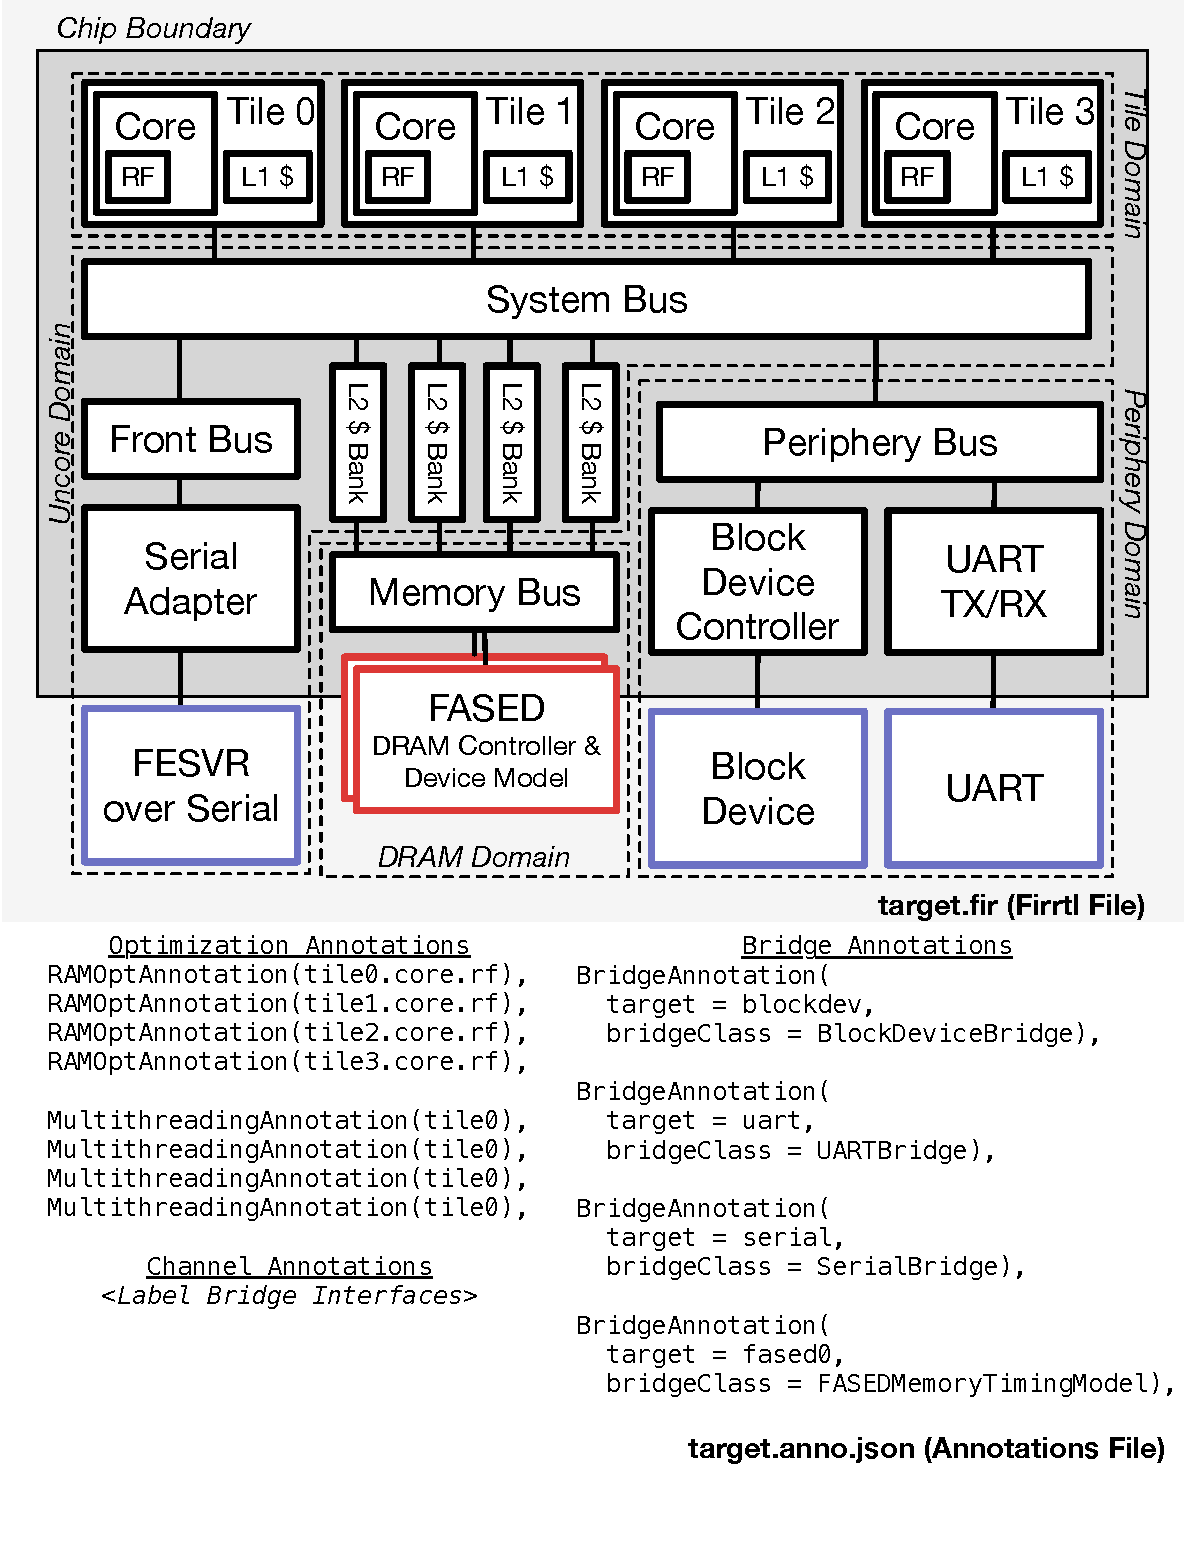
\includegraphics[width=0.99\textwidth]{figures/gg-target.pdf}
    % graffle2pdf -c gg-target midas-graphics/graffle/midas2-target.graffle figures/gg-target.pdf
    \caption{A typical Chipyard SoC passed to Golden Gate (top), and its associated Golden Gate specific
    annotations (bottom). Clock domains are shown for reference in later chapters.}
    \label{fig:gg-target}
\end{figure}

Since it does not require access to unserializable Scala
types like MIDAS, Golden Gate can be invoked as standalone application on an
elaborated target. This permits running the
compiler on a target elaborated in a different environment that may include a
different version of Chisel, FIRRTL, and Rocket Chip than those the compiler
itself depends on. We give an example invocation of Golden Gate in Listing~\ref{lst:gg-invocation}.

\begin{lstlisting}[style=shell, language=bash, label={lst:gg-invocation}, caption=An example command-line invocation of Golden Gate.]
  sbt runMain midas.stage.GoldenGateMain \
      -o <output filename> \
      -td <output directory> \
      -i  <input FIRRTL filename> \
      -faf <input FIRRTL annotations file> \
      -ggcp <Golden Gate parameters scala package> \
      -ggcs <Golden Gate parameters scala class string> \
      -E verilog
\end{lstlisting}

\section{Updated Compiler Flow}

We show a depiction of Golden Gate's compilation flow and how it modifies an
illustrative toy-design in figure~\ref{fig:gg-toolchain}.  We omit
debug-synthesis transforms, and user-provided transformations for brevity.
Golden Gate tranformations, which are statically ordered in
\texttt{MidasTransforms}\footnote{See sim/midas/src/main/scala/midas/passes/MidasTransforms.scala}, can be
roughly\footnote{Note, these terms are not currently enshrined in the
codebase.} divided into three phases:

\begin{figure}
    \centering
    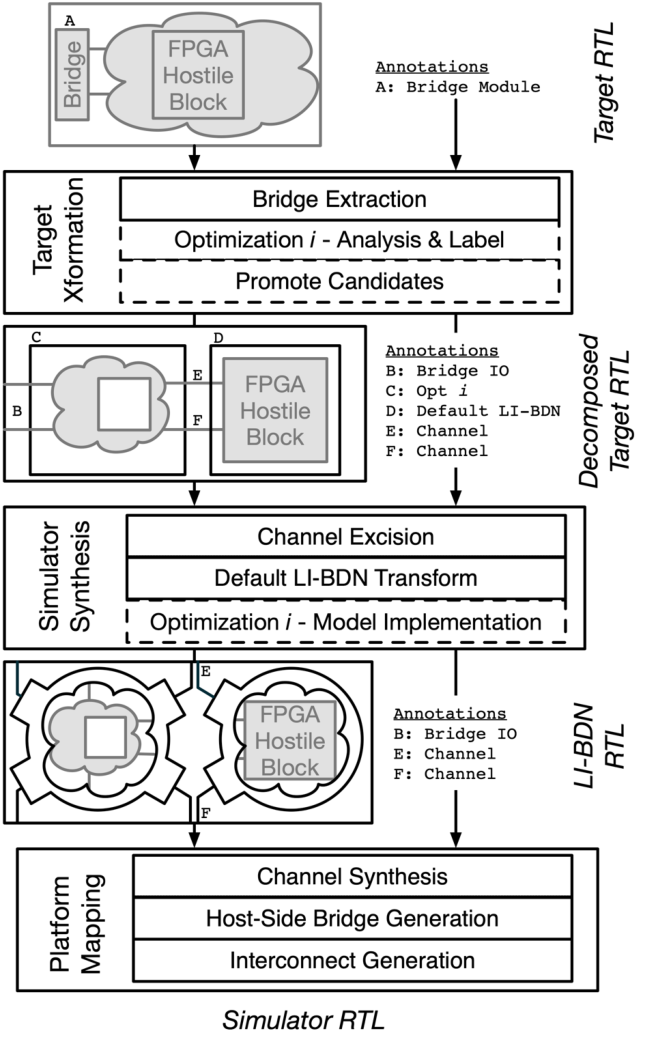
\includegraphics[width=0.8\textwidth]{figures/gg-toolchain.pdf}
    \caption{Core phases of the Golden Gate compiler and a high-level depiction
    of the transformations made to the underlying target and its annotations. The default LI-BDN transform
    is the FAME1 transform.}
    \label{fig:gg-toolchain}
\end{figure}

\begin{enumerate}

\item \textbf{Target Transformation.} Here the
module hierachy is mutated in preperation for host decoupling. Bridges are
extracted and unsynthesizable debugging constructs are replaced and
bound to a bridge interface. Primitives identified for optimization are
wrapped in modules and labelled with additional optimization annotations. These are then promoted to the top of the design hierarchy. 
All top-level modules instances correspond to units in the eventual
simulator and top-level connectivity define edges in the graph.

\item \textbf{Simulator Synthesis.} Here top-level modules are transformed
into, or replaced with, primitive LI-BDN units. On completion, the output circuit consists of a
series of unconnected unit instances. Connectivity between units is captured in
channel annotations between top-level I/O.

\item \textbf{Platform Mapping.} This consists of the Simulation Mapping and
Platform Mapping passes of MIDAS. A chisel-generated wrapper includes all
channel implementations and elaborated host-side bridge modules. The resulting output
circuit is compatible with the same FPGA projects as MIDAS-generated
simulators and plugs directly into FireSim's existing build flow.
\end{enumerate}

\subsection{Annotations}
Golden Gate relies on FIRRTL's annotation system to communicate information about the
circuit from transform-to-transform instead of an auxiliary
datastruture that persists across transformations. The main motivation for doing so was to make transforms in the
compiler robust against running lowering or optimization transformations
between them. The FIRRTL compiler framework provides callbacks for defining
how an annotation should be updated when the circuit structures it targets are
changed (a process known as \emph{renaming}). We describe the key annotations here:

\begin{itemize}
    \item \textbf{Bridge Annotations}~(\texttt{BridgeAnnotation}) label module
        instances in the target for which a custom unit will be generated.  In
        addition to labelling a target module instance, they carry a fully qualified
        class name of the Bridge Module to be generated and its optional
        constructor parameter. Finally, the annotation enumerates the names of all
        of its channel annotations.

\item \textbf{Connection Annotations}~(\texttt{FAMEChannelConnectionAnnotation}), or \emph{channel} annotations, label connections between modules that correspond to units and bridges of the simulator, and
    carry the information required to generate a channel them. This consists of
    a list of sources~(\texttt{sources}), I/O fields on the instance that drives the connection
    (i.e., they source the tokens), and sinks~(\texttt{sinks}), I/O fields on an instance
    receiving those connections. Channels carry additional metadata,
    including a globally unique string identifier~(\texttt{globalName}), as well as a case class~(\texttt{chInfo}) that
    captures target properties of connection and channel-implementation hints.
    The \texttt{chInfo} has subtypes to indicate whether the channel is latency
    insensitive and should be implemented with a queue-type channel, or is a pipe-type channel.

\item \textbf{Port Annotations}~(\texttt{FAMEChannelPortAnnotation}) label groups of I/Os in a module as corresponding to a channel source or sink.
    The list of sources or sinks in connection annotations (which point
    at instances of the module) must agree with the port annotation on the
    module itself. Port annotations are primarly consumed by transformation passes and provide the simplest means
    to look up how the I/Os of the module should be divided into channels.

\item \textbf{Model Annotations}~(\texttt{FAMEModelAnnotation}) serve a similar function to BridgeAnnotations, in that they label a
    module as being a unit. Unlike bridges, instances of the target module
    are not extracted from the design hierarchy but instead are promoted to
    the top-most level of the design hierarchy, so that they can later be
    transformed by the compiler in Simulator Synthesis.
\end{itemize}

At the start of compilation, bridge annotations are present, with connection
annotations labelling each bridge's interfaces\footnote{We note this is an abuse of the
abstraction presented by the annotation~(described above), which is fully realized only once bridges are extracted.}
Model annotations may also present alongside specific optimization annotations.

\section{Target Transformation}

The primary function of Target Transformation is to coerce the design's module
hierarchy into a form that matches the eventual simulator topology: top-level
instances, which wrap optimization candidates, map to unit instances~(nodes) and top-level connections map to
channels~(edges). Throughout this process, no host-time simulator constructs
are introduced: the RTL still directly represents the chip, albeit with a different module hierarchy.  Target Transformation
consists of all transformations before top-level connectivity is removed
(\texttt{ChannelExcision}).

Target Transformation commences with an initial lowering and optimization of the input FIRRTL, after which
the input circuit is checked for Golden Gate compatibility (namely, the circuit
presents no top-level I/O; see \texttt{EnsureNoTargetIO}). Next, Golden Gate
runs assertion and printf synthesis. Under-the-hood these do not fundamentally differ
from what was described in our DESSERT publication~\cite{DESSERT}, however
synthesized debug primitives are now bound to bridges~(more on this later).

Now Golden Gate finds all modules annotated with a bridge annotation and extracts
them~(\texttt{BridgeExtraction}). Connections to instances of
a bridge are replaced with connections to newly added
top-level I/O. Note that a single bridge module with $N$ instances will produce $N$
sets of ports at the top-level. The bridge and connection annotations are
``promoted" to point at these new top-level interfaces. Bridge annotations are then
replaced with a form of annotation that targets top-level I/O
(\texttt{BridgeIOAnnotation} instead of a module but are otherwise indentical).
Finally, connection annotations are assigned new \texttt{globalNames} to ensure they
are unique and their corresponding bridge annotations are updated to reflect
that.

Next, Golden Gate prepares for its optimization-focused hierarchy manipulations
by adding a wrapper module, the \emph{FAME wrapper}, around the existing
design~(\texttt{WrapTop}). Once optimization candidates have been removed, the
previous top-level module will become the central hub unit in the simulator.

It is at this point we envisioned custom optimization analyses would be run
find and label optimization opportunities. Currently, the multi-ported RAM
analysis is only example of this in the code base~(see
\texttt{LabelSRAMModels}).  This pass finds FIRRTL memories that have been
annotated as safe to optimize, wraps them in a module, and labels them with a
model annotation.

Then Golden Gate finds all module instances labeled with a model annotation, and
promotes them to the FAME wrapper. This process is nearly identical
to bridge extraction, but the module is not completely removed. Just as in
bridge extraction, one annotated model will produce as many top-level instances
as there were instances of the module in the design hierarchy.  At this point
the connectivity within the wrapper reflects the star-topology of the eventual
simulator: the original source module is the hub and all promoted modules and
bridge interfaces connect directly to it.

With the module hierarchy manipulations finished, Golden Gate completes Target
Transformation by fleshing out missing annotations~(\texttt{FAMEDefaults}). This primarily consists of labelling
all inter-model connectivity with connection annotations. This pass makes no
attempt to group connections into a single channel: each ground-type
connection between the hub and a spoke gets its own annotation and thus will receive an independent channel implementation.

\section{Simulator Synthesis}

Simulator Synthesis is so named because it begins introducing host-time constructs into the circuit,
most notably with the execution of the default FAME1 transformation. Simulator
Synthesis begins by removing all inter-model connectivity and replacing it
with top-level I/O~(\texttt{ChannelExcision}). Connection annotations are
promoted to point at these new interfaces. Only now are port annotations
added~(\texttt{InferModelPorts}), since connections between nodes (both bridges and models)
now uniformly target top-level I/O.  This transformation
ensures that connection annotations on instances of the same module agree as to how
ports correspond to channels. Since \texttt{FAMEDefaults} makes no attempt to
combine leaf channels into aggregate ones, this mainly serves as a consistency check on
bridge-bound channels and ensures no connection annotations have been lost.

The bulk of the complexity in Simulator Synthesis is contained in its default
FAME1 transform (\texttt{FAMETransform}). It has two fundamental tasks: first, it
transforms all top-level modules, including those that will be optimized later,
into units using a default, wrapper-based LI-BDN transform~(described
previously and shown in Figure~\ref{fig:libdn-wrapper}). The transform groups
ports into new decoupled interfaces by consuming the port annotations for the module under transformation.
References to target ports are replaced with references to the payloads
of these decoupled channel ports. Valid and ready signals are used to build out the
control circuitry shown in Figure~\ref{fig:libdn-wrapper}, however,
this logic is appended to the existing module (to avoid introducing another
level into the module hierarchy). Finally, all references to the target clock
are replaced with references to the output of a clock buffer which is responsible for driving a selectively
gated target clock.  The clock
buffer itself is left as a black box that will be implemented later for the
desired host FPGA.  The second major function of the FAME transform is to
rewire the FAME wrapper by replacing existing I/O and connectivity with decoupled
equivalents. For example, a boolean driven by a model is replaced with a three
bit interface: valid and the boolean payload is driven by the model, and ready
is driven by the I/O interface in the FAME wrapper. Connection annotations are
updated to point at the payloads of these channels.

At this point, Golden gate runs optimization transformations to replace the
default unit implementations. Since the default FAME
transformation has already decoupled the interfaces of the reference SSM, these
transformations simply replace the module body of the existing primitive LI-BDN.
Connectivity in the FAME wrapper remains unchanged.  Simulator Synthesis
concludes with some fix-up transformations which provide a default clock buffer
implementation (\texttt{DefineAbstractClockGate}) compatible with RTL
simulators, and wire up the host-clock and reset to all units in the FAME
wrapper(\texttt{ConnectHostClock}).

\section{Platform Mapping}\label{sec:gg-platform-mapping}

In Golden Gate, platform mapping is responsible for implementing all
channels (previously, known as simulation mapping in MIDAS) and elaborating
all remaining simulation collateral, such as bridges and resource interconnect
(previously, platform mapping in MIDAS). This happens in single Chisel
invocation, and produces three layers of wrapper modules, shown in Figure~\ref{fig:sim-wrapper-layers}.

\begin{figure}
  \centering
    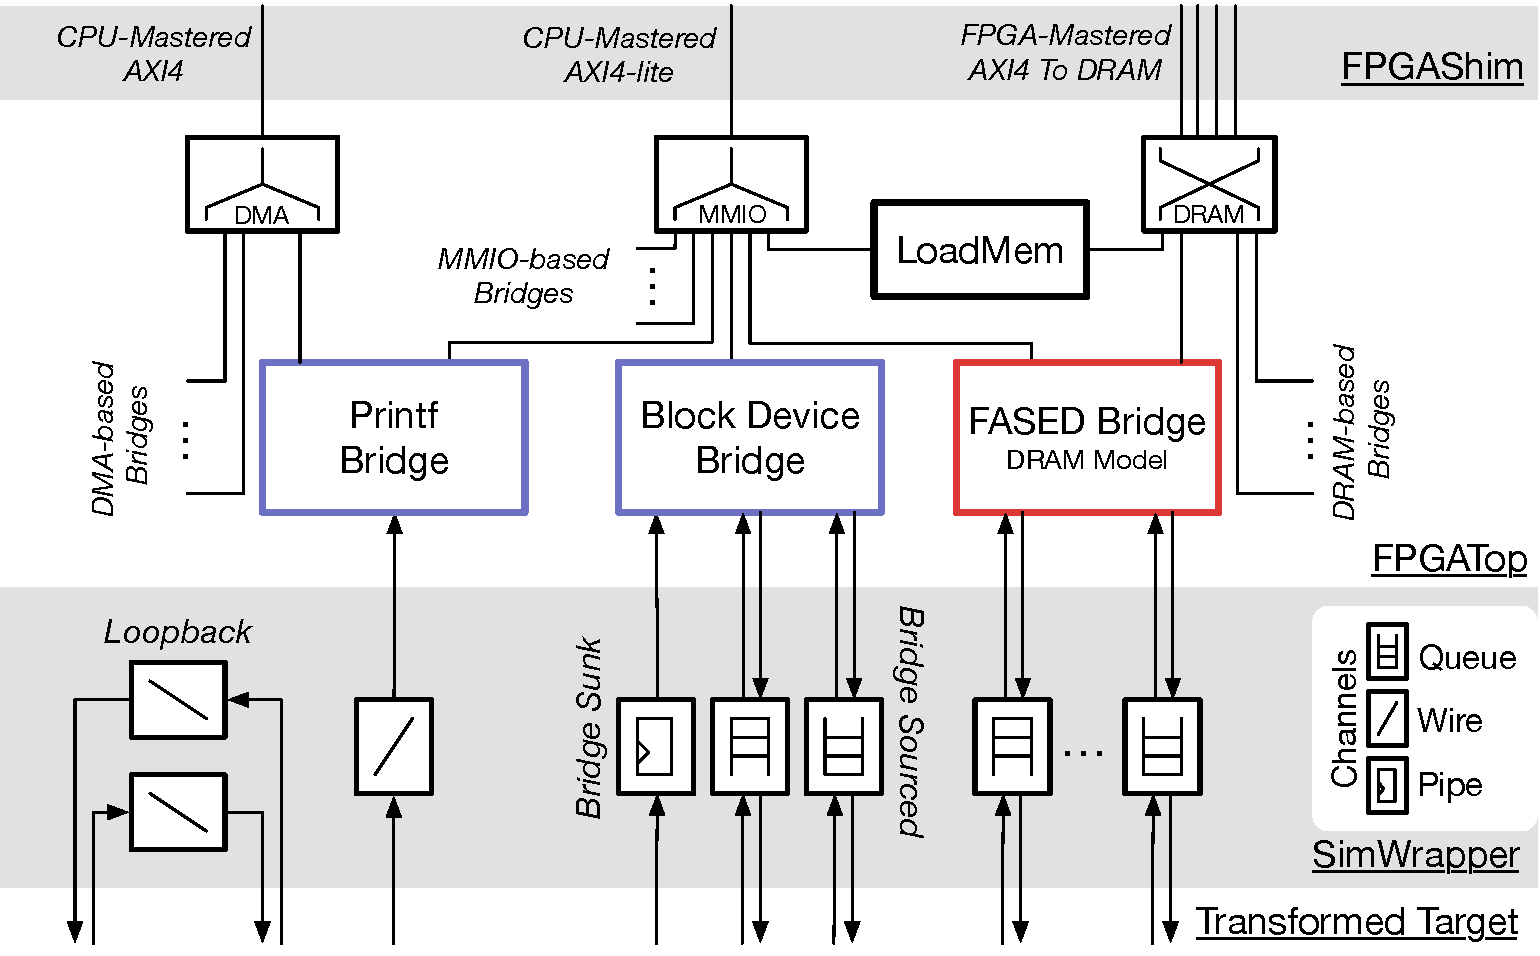
\includegraphics[width=\columnwidth]{figures/sim-wrapper-layers.pdf}
    % graffle2pdf -c wrappers midas-graphics/graffle/sim-wrapper-layers.graffle figures/sim-wrapper-layers.pdf
    \caption{The wrapper circuit generated during platform mapping, with a handful of bridges are shown for
    illustration. The host interfaces at the top (in \texttt{FPGAShim}) match those used in MIDAS. Interconnect
    between host interfaces and bridges initially was identical to that in MIDAS, but has since be augmented.
    Loopback channels, not present in MIDAS, connect two units in the transformed target.
    }
  \label{fig:sim-wrapper-layers}
\end{figure}


\subsection{Channel Synthesis}
The first wrapper layer~(\texttt{SimWrapper}) directly interfaces with the transformed RTL and instantiates
channel implementations. Elaboration of this module is driven by two inputs: the user-defined parameters instance
which, as in MIDAS, specifies properties about the host-platform. and the set of
annotations, notably connection annotations, labelling the now transformed target.
Each connection annotation will corespond with a channel implementation, however how that channel
is bound depends on the \texttt{sources} and \texttt{sinks} enumerated by the annotation.
Connection annotations that possess both \texttt{sources} and \texttt{sinks}
connect two models in the transformed RTL; these are \emph{loopback} channels
that drive an input and an output interface on the transformed target. Conversly,
annotations that possess an empty \texttt{sources} or \texttt{sinks} parameter
are sunk or driven by a bridge module, respectively. In these cases, the
channel implementation has its dequeue or enqueue side
interface exposed to the next wrapper-layer of the module hierarchy.

In all cases, the type of channel generated is parameterized by the
\texttt{channelInfo} field of the connection annotation. Target-decoupled channels, as in
MIDAS, always instantiate a model of a fully decoupled, two-deep queue. Pipe
channels have a configurable latency. Default bridge implementations always
emit channel annotations with latency equal to one to improve FMR, and to maintain the
performance characterisitics of legacy MIDAS simulators. When no additional
models are extracted (i.e., the simulator consists only of the hub unit and
bridges) the expected FMR is identical to MIDAS.
When additional units are extracted, they are always directly wired to the
hub, since the compiler currently cannot find and extract registers~(that is to
say, \texttt{FAMEDefaults} labels these channels as wire-type). This has
the effect of making all multi-model simulators execute with an FMR of at least two\footnote{It is possible to build
simulators with unity FMR, if an optimized model's outputs can runahead. At time
of writing, we have no such implementations.}.

\subsection{Bridge Instantiation}
The next-level of the module hierarchy~(\texttt{FPGATop}) corresponds to the wrapper
circuit generated in MIDAS's platform mapping. I/O on this wrapper module consist of AXI4 interfaces
to drive host-DRAM memory systems, and to support CPU-driven MMIO and DMA.
Instead of using an endpoint map, Golden Gate iterates through each bridge
annotation and reflexively invokes the constructor for the requested
BridgeModule. I/O between the elaborated
bridge instance and the simulation wrapper are connected by looking up the
corresponding channels via their \texttt{globalName} fields.
Resource-interconnect generation is identical to MIDAS's, and for the same
input design, the emitted header is the same. All MIDAS endpoints were ported
to use the new Bridge system, without changing existing host software.

\subsection{Platform Wrapper}
The last level of wrapper module is an FPGA-specific shim layer. The user
selects their desired shim through the parameters instance. This serves as an
opportunity to introduce FPGA-specific hardware and modify interface names to
slot into an FPGA shell project. We note that this top-level module could
instantiate all of the IP required to define a complete FPGA project~(as in
SiFive's FPGA shells repository), but none of our shims do so presently. The
class for this wrapper module can be defined outside of Golden Gate and
provided by a user wishing to support a non-standard FPGA.

\section{ICCAD 2019 Golden Gate Publication}

Armed with the machinery to selectively extract and reimplement FPGA-hostile
components of the target design, in our ICCAD2019 we set about optimizing
multi-ported RAMs~(we previously introduced this example in
Section~\ref{sec:iron-law}).  ASIC multi-ported RAMs are a classic culprit of
poor resource utilization in FPGA prototypes, as they cannot be trivially
implemented in BRAM and are instead decomposed into LUTs and
registers~\cite{FPGAGap2}.  While using double-pumping, BRAM duplication, or
FPGA-optimized microarchitectures~\cite{MultiportXOR} can help, here we used Golden Gate to
replace the SRAM with a multi-cycle unit to further reduce resource
utilization. This optimization implements a target memory possessing $M$ asynchronous read ports and
$N$ write ports with a single time-multiplexed dual-ported BRAM. In contrast to the static time-multiplexing schemes described
by Pellauer et al.~\cite{APortNetworks} and Dwiel et al.~\cite{fabscalarfpga}, our optimization can decouple arbitrary target
memories and replace them with an optimized model without any constraints on the structure or timing of the
target design.

In order to rigorously verify optimizations, in our ICCAD publication we also
introduced a bounded-model checking flow, called Latency-Insensitive Model
Equivalence~(LIME), hosted in UCLID5~\cite{UCLID5}, to formally verify that
optimized models are valid LI-BDNs implementations of their reference RTL.  Our
manipulations of the module hierarchy were in direct service of this goal, as
any extracted RTL module could trivially serve as the reference RTL for a
verification flow. In our ICCAD paper, we used LIME to verify only our RAM
optimization, however, there is nothing that precludes applying LIME to
\emph{all} reference-unit pairs in a simulator. This verification flow could be
run in parallel to FPGA compilation, providing a multi-hour window to catch
potential bugs before a simulator is deployed to FPGA.

\begin{figure}
  \centering
    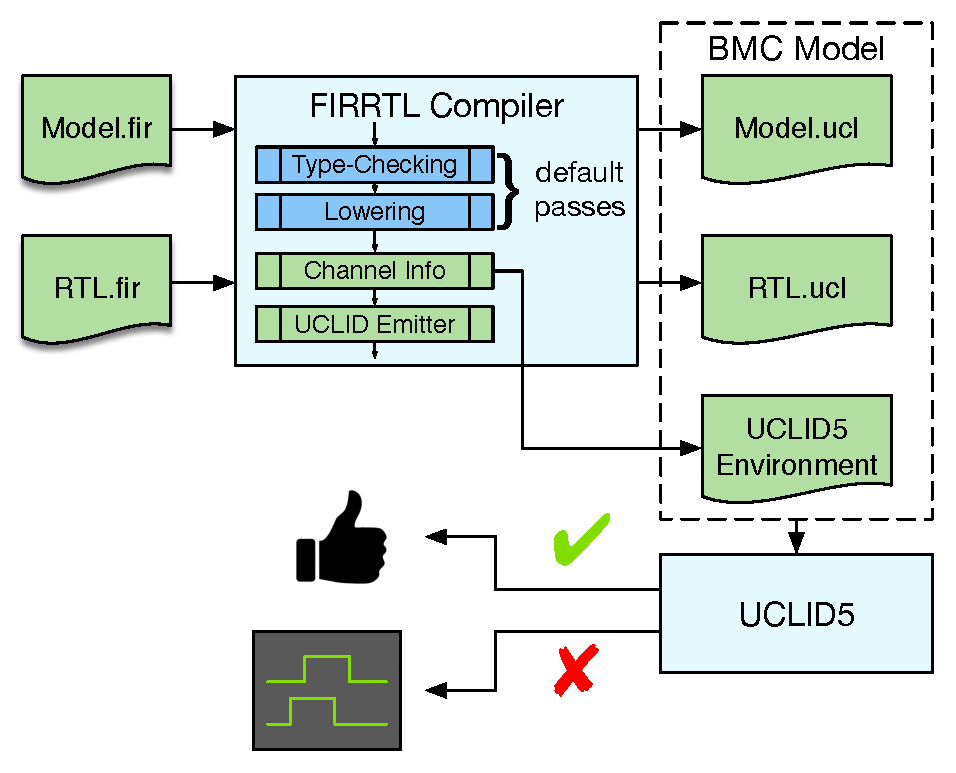
\includegraphics[width=\columnwidth]{figures/lime_flow_small.pdf}
    % -c default midas-graphics/graffle/lime_flow_small.graffle figures/lime_flow_small.pdf
    \caption{The LIME model checking flow. In LIME, FIRRTL for a unit and its
    reference SSM are lowered and emitted as UCLID5 representations. A
    Python-based enironment generator (not shown), consumes channel information
    emitted by the compiler to generate test environments for PI, GC, and NED.
    If the unit is not a valid LI-BDN, LIME produces a waveform counterexample
    that demonstrates how the property under test was violated.
    }
  \label{fig:lime-flow}
\end{figure}


The LIME model checking flow and RAM optimization first described in our
ICCAD2019 paper are primarly contributions of Albert Magyar and are described
at length in Chapters 6 and 7 of his dissertation.



\chapter{Target-to-Host Bridges And Their Performance Considerations}\label{sec:bridges}

While our ICCAD 2019 publication focussed on how to flexibly introduce resource
optimizations without changing target behavior, our rework of MIDAS's endpoint
system was the second major development in the compiler and was implemented in
the months thereafter. If Golden Gate is to FPGA hosts as verilator or VCS is
to CPU hosts, then target-to-host Bridges can be best thought of as Golden
Gate's analog of the Verilog Procedural Interface~(VPI): they provide a
side-channel mechanism for the user to inject arbitrary, often unsynthesizable
modeling resources anywhere in their design. In practise, many features
implemented using VPI can re-implemented for FireSim using bridges: the
black-box wrapping a VPI call can be annotated as a bridge. When the design is
simulated in a conventional RTL simulator the VPI implementation used, when it
is simulated in FireSim its bridge implementation is used.

Bridges serve the same purpose as endpoints but differ in three primarys ways:
\begin{enumerate}
    \item They are integrated into the target as modules, and elaborated as
        part of the target.  Bridges can be instantiated at any level in the
        design hierarchy, not simply in the top level.  So while Bridges can be
        used like endpoints to provide I/O models for the dut, they enable many
        other applications: They can be used to instantiate units that serve as
        monitors or golden models, to verify parts of the target in-situ. They
        can be used to provide alternate implementations of expensive or
        unsynthesizable target modules deep in the module hierarchy. This
        provides a second means to introduce resource optimizations.


    \item Their elaboration-time parameters are serializable. This permits elaborating 
        the target in a separate process to golden-gate invocation.

    \item They can easily parameterized by their instantation context. With
        endpoints, it was difficult to disambiguate between multiple intances
        of the same type of endpoint (e.g., different channels of the sameDRAM
        subystem all appear as AXI4 interfaces on the top-level I/O). Conversly,
        when bridges are instantiated they can accept arbitrary parameters that
        may only be known at their instantiation site (e.g., the number of
        outstanding memory requests that may be made on an AXI4 interface).
\end{enumerate}

\section{Achieving Good Performance: The Crux Of Bridge Design}
Of course, to support VPI-like functionality on an FPGA is a fundamentally more
challenging prospect due primarily host-transport considerations and speeds at
which the simulator is executing. A naive bridge implementation, could reuse
same VPI source code hosted as part of a BridgeDriver, the driver could read
I/O values from the FPGA, invoke the VPI function on those values, and then
write updated values to the FPGA (the bridge Module would emit these new values
as one-or-more tokens).

Let's consider the performance of this approach for VPI call that models a
purely combinational function~(i.e., it has no target state it must update from
timestep to timestep): this represents both the simplest case to analyze and
has the worst-case simulation performance. Lets consider a simple hybrid
CPU-FPGA host system, shown in \TODO{figure}.

Where, l is the inter-FPGA-CPU transport latency, which we'll assume to be the
time required to move all bits of an input token to the CPU or all bits of the
output tokens back to the FPGA. In practise $l$ scales with the size of the
tokens due to serialization and deserialization latencies, but we'll neglect
this for now.
$p$ is the latency of invoking the function that models the
combinational function, essentially the time it takes to run code that
implements the VPI call on the host CPU.
$f$ is the period of one FPGA cycle.

FMR in this resulting system, is given \TODO{by}.

In this system, in order to maintain unity FMR, $2l + p < f$, a practical
impossiblity -- as even the time required to move the token across FPGA-fabric
will require some multiple $f$ seconds. To make this more concrete, consider
typical times on an EC2 F1 host. Empirically, we've measured MMIO read and
write latencies, specifically the latency between a BridgeDriver calls
simif\_t::write or simif\_t::read, and when that function returns as taking
\TODO{seconds} \TODO{seconds} respectively. Assuming, $f_{fpga}$ of 100 MHz, a
readily achievable frequency for multicore Rocket designs with shared L2
caches. In this case, even if we assume $p = 0$, simulator FMR must exceed
\TODO{10}.

Another artificial but illustrative case to consider is when $l = 0$, and $p$
is non-zero (this is roughly analagous to having a bridge directly connected to
the hub-unit, or using using flow-through queues as the channel implementations). Given a CPU-host frequency
of, this gives exactly \TODO{cycles} on the CPU host to model the combinational
function.

A final illustrative case to consider, is one in which a bridge is purely a
sink or source of tokens. Here there is no causal loop between parts of the
simulator hosted on the CPU and on the FPGA~(we assume no other side channels).
and the bridge can decouple arbitrarily from the the rest of the simulator.
Even still, these bridges can result in FMR penalties due to rate-limiting, if
there is insufficient bandwidth to move tokens between the FPGA and CPU. We update our model,
to suppose the host can support $K$ GB/s of read and write bandwidth.
update our model, such that such.

There is hope for the simulation designer, assuming they can exploit one of two key properties. 
The first is target latency of the underlying causal relationship.~\TODO{clocks} A combinational path is the worst case
as for the purpose of delay-less RTL simulation, as this is essentially zero. If we consider a loopback with
path with $t_l$ registers, to maintain unity FMR, our unit would need to meet:

The other properties is that often $p$ is non uniform, for many cycles, a unit
may have nothing to do here $p$ can apporach zero.  In otherwords, it might be
acceptable to model even something like a combinational function in software,
if that function is evaluated infrequently.

These analyzes become vastly more complex when accounting for variability in
host timings, non-uniform FMR introduced by other simulation components, an
contention for shared simulation resources, but it highlights \TODO{4} general
strategies for improving bridge and unit performance.

To summarize, the simulator design has four major tools they can deploy:
\begin{enumerate}
    \item Reduce $l$.
    \item Reduce $p$.
    \item Exploit or increase $t_l$.
    \item Exploit or increase $d$.
\end{enumerate}


These are not by any means new observations---they are fundamental properties
of any program running over a distributed host. Generalizations of this
analysis can be found through the distributed computing literature, especially
in PDES, where causality constraints between parts of a distributed simulation
impose a precise coupling between pieces of the simulation. Moreover, these
challenges are well known in the commercial hardware-emulation space, where
special care is given to parts of the emulator that span FPGA-and-CPU.

However, we feel it is important for bridge designers to understand the
constant factors at play (i.e., the expected latencies and bandwidths they must
design around) when writing a bridge) when designing for FireSim specifically,
and give examples of how to overcome these limitations.  To this end, we
describe three notable bridge implementations in FireSim. FESVR-over-TSI, a
low-bandwidth bridge relies on regularizing infrequent interactions;
Synthesized Printfs, a sink-only bridge, that uses FPGA-DMA to supply the need
host-bandwidth to prevent simulation stalls; and FASED memory timing models,
which uses FPGA DRAM as a backing store and attempts to hide the latency of
FPGA-DRAM access by modelling DRAM memory systems at the DRAM controller
boundary (as opposed to modelling the DRAM devices at the SoC boundary
interface).

\section{FESVR-over-TSI Bridge}
At time of writing, all target designs supplied in Chipyard (and present in
FireSim previously) are \emph{tethered}, and cannot boot standalone. The RISC-V
Frontend Server (FESVR) is responsible for managing the early stages of boot.
It keeps the target HARTs under reset, while it loads a binary into target
DRAM, (e.g., the Berkeley Boot Loader\cite{BBL} and a linux kernel, or a
baremetal binary). During execution, FESVR monitors the target by periodically
polling \texttt{tohost}. The SoC can proxy certain types of I/O, like printfs)
to FESVR, by setting tohost to a specific value, and providing an address to a
buffer that FESVR can decode and process. While we do not use these features,
since we have our own IO device models, FESVR only remaining responsibility is
to detect when an SoC has successfully "powered down", so that it may signal
the end of the simulation.

The tether-serial interface (TSI), is one transport layer implementation for
FESVR requests that implements FESVR requests as encoded TileLink transactions
it serializes over a narrow link. A receiver, bound to the front-bus of the
SoC, deserialize and decodes these TileLink transactions (e.g., a 32-bit read
to tohost) and issues them to the SoC's memory system. Responses are handled in
reverse.

The Bridge implementation of TSI is perhaps the simplest one deployed in
FireSim. To enable simulations to run at unity FMR, while remaining
deterministic, the bridge imposes that FESVR requests may only be made visible
at fixed intervals in target time. At the start each interval, FESVR is free to
make a request; the bridge encodes the request into a series of tokens,
allowing the simulator to advance. When tokens for the request have been
consumed, the BridgeDriver generates null-tokens for the remainder of the
interval. When the SoC produces a response, it is enqueued in the bridgeModule.
At the start of the TSIBridgeDriver processes the response, taking as long as
it requires, and produces the next request. This process repeates ad infinitum
until, during a poll of \texttt{tohost}, FESVR detects powerdown, and signals
to the bridge the simulator should terminate.

While this implementation does not attempt to hide the latency of FESVr
processing the request, it minimizes the number of FPGA MMIO requests the
bridge driver must make. By selecting a large polling interval~\TODO{value},
simulator FMR, in the absence of other host-time stalls, approaches unity.

\section{Synthesized Printfs}

Synthesized printfs are unidirectional, specifically it is implemented using a
sink-only bridge, a common pattern among bridges that support
intrumentation-like features (other examples include TracerV instruction
tracing, synthesized assertions, and AutoCounter). Since unidirectional bridges
can decouple completely from the rest of the simulator, achieving good
performance depends on avoiding rate limitations. In other words, to avoid
simulation slowdowns, tokens must be processed at the rate at which they are
being generated by the rest of the simulator.  The load a FIRRTL
\texttt{printf} exposes to the simulator is affected by two principle
considerations. Its activity factor, the fraction of cycles during which the
printf is enabled, and its bitwidth, the combined width of all fields in its
format string. Bridge throughput can be limited by CPU-FPGA DMA bandwidth,
host filesystem bandwidth, or driver-side printf formatting throughput.

During printf synthesis, Golden Gate collects all annotated printfs, and
punches a connection through module hierarchy to a central, top-level bridge.
Each printf is represented by an aggregate type consisting of a boolean enable,
and a variable number of arguments that populate the format string of the
printf. In a given cycle, the values on all of these interfaces
together are concatenated into a single token.

The current bridge implementation uses DMA to provide adequate bandwidth for
printfs that either wide or frequently active. The bridge buffers tokens in
a very deep fifo, the allow the bridge to tolerate latencies between services,
and to allow for good DMA batching.  To save bandwidth in periods of low
activity, a cycle counter tracks the number of consequetive tokens received
with no printfs enabled.  When at least one printf is active, a null-token is
buffered indicating the number of idle cycles between active printfs. In the
next cycle, the bridge buffers the active printf token. For systems with many
printfs with uncorrelated enables, these tokens can be sparsely populated
wasting DMA bandwidth, but we note this could be alleviated by using multiple
bridges.

While the bridge module dequeues and buffers up tokens, the driver periodically
polls to see if the FPGA-side is full, and if so, drains the buffer with a
\TODO{large} DMA request. Here the driver has two modes: it can write out the
token stream to file directly \TODO{"binary"}), or decode the token stream into
formatted print messages. Depending on the number and types of arguments,
formatting the string can dramatically reduce simulation throughput, To
overcome this, users can specify a region of interest over which to collect
printfs, or use the unformatted binary mode, and rely on selectively
post-processing the output file.

\section{FASED Memory Timing Models}

Modelling large, off-chip memory systems, like DRAM, requires special
consideration to produce high-performance simulators. On one hand, DRAM is
frequently accessed and has relatively low latency -- the fastest DDR3 and DDR4
speedgrades have CAS latencies, the number of cycles after a
column access command the read data will appear on the data bus, of \TODO{14}
and \TODO{?} cycles respectively.  These latencies are much too small to allow
modelling DRAM accesses in software. On the other hand, DRAM memory systems
cannot be synthesized into FPGA fabric --- they are simply too stateful. So,
the only means to host DRAM memory timing models in an FPGA based emulator is
to use the FPGA's DRAM memory system. FASED is responsible for providing
high performance~(FMR), DRAM memory system models in FireSim by doing exactly this.
FASED is described in greater detail in our FPGA2019~\cite{FASED} publication, here
we shed more light on simulation performance considerations not covered in the paper.

Using FPGA-attached DRAM to model DRAM memory systems in the target is not
novel. FPGA prototypes will often substitute the ASIC DRAM controller with
either soft or, as is customary now, hard FPGA DRAM IP. This can produce memory
system timings that wildly differ from the proposed target design, but this may
be acceptable if the prototype is being used as a functional platform for
software development and not for performance validation. Producing timing faithful
simulations of the target typically falls to hardware emulators, where the
target DRAM controller can be simulated with little or no modification and attached to models of DRAM
devices. Here, a natural approach is to provide timing models for DRAM devices that leverage FPGA-attached DRAM
as a backing store, and bind them to the interface presented by the target SoC.

To provide a higher performance, and more general purpose means to simulate
large off-chip memory systems, FASED models both the DRAM devices and the DRAM
controller that schedules over them, by binding to an AXI4 memory controller
interface in the SoC, instead of the DRAM device side interface. This is more
general purpose in that it can be used to model any AXI4 memory slave device,
making it possible to write abstract models (like latency pipes) but
also detailed timing models for other memory technologies, in a way that reuses
a functional model responsible for issuing transactions to the FPGA memory
system. This approach can also enable writing higher-performance simulators, as
it provides more target-latency to hide host-memory accesses. In practise, the
AXI4 read transaction will need to be scheduled, decoded into one or more DRAM
commands, which must wait on other commands before the read command must be
issued. Only now is the CAS latency is realized before any additional latencies
in the controller to return the data back through the AXI4 interface. Under
loaded memory systems, or when a column access does not hit in an open DRAM
page, the target latency of of the read transaction can be many times that of
CAS latency, this may be sufficient to hide the host DRAM access entirely,
allowing the simulator to run at unity FMR.

\section{Organization \& Operation}
We show the block diagram of a FASED timing model in
Figure~\ref{fig:fased-block-diagram}. FASED instances leverage a
timing-functional model split commonly deployed in microachitecture simulators
\TODO{citation needed} and prior RAMP work~\cite{FAST, RAMPGold}. Timing
accuracy and simulation determinism is provided by treating the timing model
and functional model as two distinct simuation units bound together with
wire-type channels.  The host request scheduler, response staging unit, and the
backing FPGA memory system together constitute the functional model. The
host-request scheduler snoops requests in tokens bound for the timing model,
and issues them to the host memory system.  As responses arrive, they are
queued up in the reponse-staging unit.  These blocks are written in host-time
RTL and directly act on simulation tokens.  Conversly, timing models are
written as a single module of target-time RTL, which is tranformed into a
patient SSM using a simplified FAME1 transform. This makes it easier describe
complex target behaviors, and opens the door to reusing compiler optimizations
in the future. Timing models request host responses using the target AXI4-ID as a key
presented over BReq and RReq interfaces~(for write and read responses
respectively). From the timing model's perspective, the queuried response is
presented to the timing model in the next target cycle. If the reponse for the
requested ID is not yet available, the functional model does not produce the
next token, causing the timing model to stall.

\begin{figure}
    \centering
    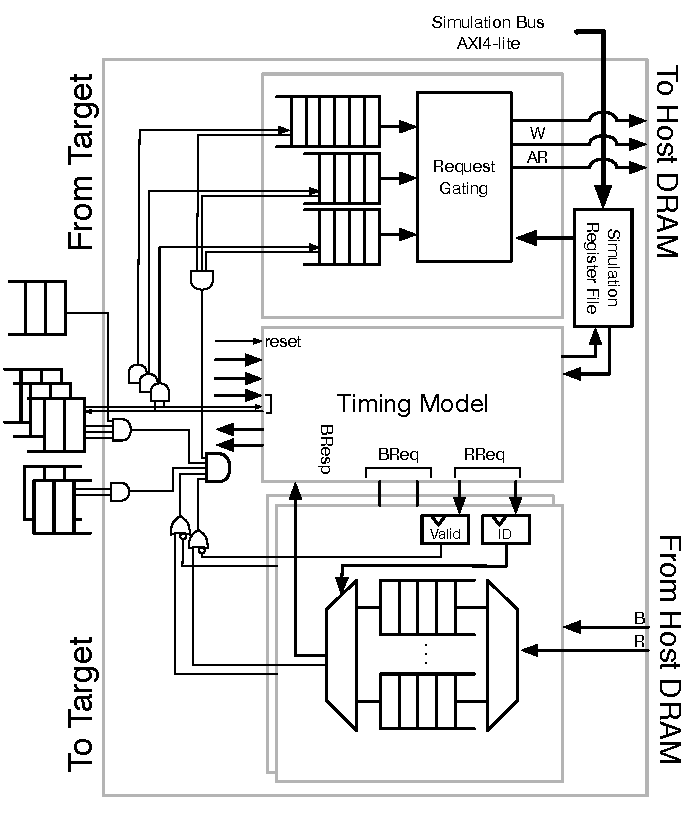
\includegraphics[width=0.99\textwidth]{figures/fased-block-diagram.pdf}
    % graffle2pdf -c full midas-graphics/graffle/memory-model-block-diagram.graffle figures/fased-block-diagram.pdf
    \caption{A timing-model-agnostic block diagram of a FASED memory model with
    all critical control signals.}
    \label{fig:fased-block-diagram}
\end{figure}

How this procedure allows FASED to deterministically model memory system
timings is best illustrated with an example -- to this end, let's consider a
FASED instance us consider modeling a memory system with single cycle of
latency. This is depicted in Figure~\ref{fig:model-operation}.  Suppose we have reached the first
read request issued to the memory system~(Figure~\ref{fig:model-operation-1}). Let this be host and
target cycle 0. When the timing model accepts this request, it is snooped by
host-request scheduler. Simultaneously, the timing model makes a request to
host-response staging module as it needs to reply to the read in the next
target cycle.

In host cycle 2~(Figure~\ref{fig:model-operation-2}), the host-response staging module
cannot produce the associated host response, since it has yet to
be issued, and so generates no fToken, stalling the timing model.
In parallel, the host-request scheduler issues the required read to
the host memory system. While the host-response staging module
waits, the timing model stalls. If the host memory system responds
in K cycles, at host cycle K + 1~(Figure~\ref{fig:model-operation-3}), that response is received.
In cycle K + 2~(Figure~\ref{fig:model-operation-4}), the host-response staging module
produces an output token, targetFire is asserted, and target cycle
1 executes. Here the timing model forwards the data directly into
its output token. From the target’s perspective, the read occurred
in a single cycle, however, the cycle was executed with an FMR of
K + 2. As the latency of the target increases, FMR decreases and
approaches unity. If the target memory system is strictly slower
the host memory system, the instance executes at unity FMR.

\begin{figure*}[t]
    \vspace{-0.25in}
	\centering
    \begin{subfigure}[t]{0.23\textwidth}
        \includegraphics[width=\columnwidth]{figures/model-operation-1.pdf}
        % graffle2pdf -c 1 midas-graphics/graffle/memory-model-operation.graffle figures/model-operation-1.pdf
        \caption{}
        \label{fig:model-operation-1}
    \end{subfigure}
    \begin{subfigure}[t]{0.24\textwidth}
        \includegraphics[width=\columnwidth]{figures/model-operation-2.pdf}
        % graffle2pdf -c 2 midas-graphics/graffle/memory-model-operation.graffle figures/model-operation-2.pdf
        \caption{}
        \label{fig:model-operation-2}
    \end{subfigure}
    \begin{subfigure}[t]{0.24\textwidth}
        \includegraphics[width=\columnwidth]{figures/model-operation-3.pdf}
        % graffle2pdf -c 3 midas-graphics/graffle/memory-model-operation.graffle figures/model-operation-3.pdf
        \caption{}
        \label{fig:model-operation-3}
    \end{subfigure}
    \begin{subfigure}[t]{0.23\textwidth}
        \includegraphics[width=\columnwidth]{figures/model-operation-4.pdf}
        % graffle2pdf -c 4 midas-graphics/graffle/memory-model-operation.graffle figures/model-operation-4.pdf
        \caption{}
        \label{fig:model-operation-4}
    \end{subfigure}
	\centering
    \caption{A FASED instance simulating a single-target-cycle read. Data
    tokens carry target transactions~(their target-valid bit is set) whereas
    empty tokens do not carry a target transaction.}
    \label{fig:model-operation}
\vspace{-0.20in}
\end{figure*}

\subsection{Simulation Performance Case Study}

\begin{table}[t]
\centering
    \begin{tabular}{c@{\hskip 0.1in}
        S[table-format=3.2]@{\hskip 0in}S[table-format=3.2]
        S[table-format=3.2]@{\hskip 0in}S[table-format=3.2]
        S[table-format=3.2]@{\hskip 0in}S[table-format=3.2]}
    \hline
        \textbf{Benchmarks} & \multicolumn{2}{c}{\textbf{Insns~(T)}} & \multicolumn{2}{c}{\textbf{D\$ MPKI}} & \multicolumn{2}{c}{\textbf{I\$ MPKI}} \\
    \hline
        perlbench & 2.98 & 2.99 & 9.0 &  8.9 & 10.0 & 10.1 \\
        gcc & 2.43 & 1.35 & 36.6 & 29.5 & 9.7 &  11.1 \\
        mcf & 1.60 & 0.91 & 97.9 & 80.9 & 0.1 &  0.1 \\
        omnetpp & 1.11 & 1.11 & 56.9 & 56.6 & 9.3 &  10.4 \\
        xalancbmk & 1.21 & 1.21 & 62.9 & 62.9 & 7.9 &  7.6 \\
        x264 & 4.55 & 4.55 & 3.0 &  3.0 & 2.9 &  3.0 \\
        deepsjeng & 2.51 & 2.14 & 8.7 &  8.2 & 15.4 & 15.3 \\
        leela & 2.59 & 2.59 & 5.8 &  5.8 & 1.5 &  1.5 \\
        exchange2 & 3.24 & 3.24 & 0.0 &  0.0 & 0.1 &  0.1 \\
        xz & 9.41 & 2.25 & 19.8 & 15.7 & 0.2 &  0.1 \\
    \hline
    \end{tabular}
    \caption{Dynamic instruction counts and L1 MPKIs of SPEC2017int rate and speed~(single threaded), respectively.}
    \label{tbl:spec-insns}
\vspace{-0.35in}
\end{table}

\subsubsection{Target Designs}\label{sec:target-parameters} Our target designs
are derived from the Rocket Chip generator~\cite{rocketchip}, which contains
Rocket, a single-issue in-order scalar core implementing the RISC-V
ISA~(RV64IMAFDC). Rocket Chip
has been taped out over a dozen times for both research and commercial
purposes. In our
experiments, we use the default
configuration of Rocket Chip, which includes
a \wunits{16}{KiB} L1 I\$, a blocking \wunits{16}{KiB} L1 D\$, and 32-entry
fully-associative L1 I and D TLBs. We only change the default configuration to
increase the number of performance counters and deepen the L2 TLB to 1024 entries.

At the system level, our targets consist of single or quad-core instances
of Rocket Chip (labeled SC or QC), composed with either a latency-bandwidth pipe
or a quadruple-rank DDR3-2133~(14-14-14) FCFS or FR-FCFS
DRAM models over a 64-bit AXI4 bus. In all targets, the simulated system has
16 GiB of DRAM capacity. Additionally, two targets include a 4 MiB
LLC model~(labeled LLC). In the target's periphery, we have a UART and block
device that interact with simulation models co-hosted in software.

\subsection{An Overview SPEC2017int On Rocket}
In our experiments, we run SPEC2017 intrate and intspeed suites with reference
inputs, cross-compiled for RISC-V systems with the \texttt{-O2} flag.
Intspeed benchmarks require as much as \wunits{16}{GB} of memory, while intrate
benchmarks require \wunits{2}{GB} per copy.  In Table~\ref{tbl:spec-insns}, we give each suite's dynamic instruction
count and L1 MPKIs when running on the Rocket configuration of
Section~\ref{sec:target-parameters}

\input{tex/tables/simulator-performance.tex}

Table~\ref{tbl:intrate-simtimes} gives the
host-execution times and execution speeds for a handful of SPEC2017 runs. The
targets with DDR3 models consistently run at rates above \wunits{100}{MHz}. Theoretically,
FASED instances can operate at the host frequency~(160 MHz) if the functional model can always serve timing model requests in time.
On our host, reads and writes take on average 47
and 37 cycles, respectively, when unloaded.  These latencies have
a significant effect on simulator performance when modeling a single-cycle memory
system as that host latency is fully exposed to the simulator, but
they have relatively little impact
when modeling a realistic DRAM system
whose latency~(cycles) is similar to that of the host.
Instances with LLCs fall between these extremes: LLC hits are fast in
target time and thus expose the host-DRAM latency to simulator, while
misses present sufficient target-latency to hide the host-DRAM access.
For our DDR3-2133 target memory system, reads take 20, 34, and 48 cycles for
row hits, closed row, and row misses, respectively. These latencies are large enough that many accesses can be
served by the functional model before the timing model requires them, eliding simulator stalls.
Ironically, modeling a slower DDR-speed-grade slows down the simulator: since $t_{CS}$ is smaller, reads complete in fewer target
\emph{cycles} despite taking more target \emph{time}.

\subsection{Limitations}
The downside of this approach is that FASED replaces the target memory
controller, whereas a device-based model does not. Thus, while FASED provides a
more accurate model of DRAM memory timings they will not match that of the ASIC
memory controller, and could possibly differ wildly, if their memory access
schedulers are substantially different. One way to ameloirate this, is to
instantiate ASIC DRAM controller directly within a new FASED memory timing
model\footnote{In the future we plan make this easier by breaking FASED into
two libaries -- an inline, AXI4-memory slave bridge, which can be inserted
between any AXI4 master and slave, and a library of timing models that can be
instantiated in the target design these timing models will expose their
configuration and instrumentation registers to a second bridge. Users who wish
to simulate their own memory controllers can then instantiate just the
functional model.} While this will produce timings that exactly match that of
desired memory system, FASED's functional model can still mask datapath bugs in
the DRAM controller RTL since the functional model will always return correct
data, where as a device-based model would correctly simulate the erroneous
behavior.



\chapter{Support for Systems With Multiple Fixed-Frequency Clocks}\label{sec:static-multiclock}

%If lack of simulation realism was one of the largest deterrents to adopting FireSim,
%modeling rationally related clocks is a stepping stone to building systems
%with dynamically scaling ones.  Useful for doing performance modeling.

%https://patents.google.com/patent/US6785873B1

Until now all Golden Gate and MIDAS-generated simulators modeled systems with a
single clock domain. Anecdotally, the lack of support for simulating targets
with more than a single clock has been the most common criticism of FireSim
offered by potential users, many of whom turn to using a conventional FPGA
prototype. The criticism is well justified: forcing the outer memory hierarchy
to run at the same frequency of the cores results in a memory hierarchy that
can sustain artificially high bandwidths at lower latencies.

To date, the only effort to validate FireSim performance against a silicon
implementation was conducted by Lee and Waterman~\cite{VLSIFireSimEval}. They
compared SPEC2006 Integer results collected from the HiFive
Unleashed~\cite{HiFiveUnleashed} against an equivalent design running on
FireSim. While the FireSim-collected SPEC score fell within 2\% of the
HiFive Unleashed's, the largest single-benchmark difference was 10.7\% for \texttt{429.mcf}, a
benchmark with infamously poor memory locality (its working set has been
measured at 680 MB\cite{SPEC2006WorkingSet}). The FireSim variant differed in that
it used non-standard UC Berkeley I/O devices (and backing FireSim Bridges) and a
FASED memory timing model instead of an ASIC DRAM memory controller.
However, the most pertinent difference between the two platforms is that the
HiFive Unleashed coreplex and memory hierarchy spans three clock domains. Tiles
run at the fastest frequency~(1.5 GHz in their study), the uncore runs at half
this frequency~(75O MHz), and the DRAM memory system, capable of 2400 MT/s
(resulting in a 600 MHz controller clock in the Unleashed), sits in its
own clock domain behind an asynchronous crossing\cite{FreedomU540}. To model
these domains without native support for multi-clock simulation, they resorted
to adding additional buffering between the L2 and the inner caches, and scaling
FASED latencies to match the times expected from a DRAM controller
running at a slower frequency. Systems like the Freedom Unleashed, which do not actively scale frequencies
after boot, are relatively common. For these systems, support for multiple statically defined clocks
would suffice to resolve this performance discrepancy.

To implement this feature, a natural place to look for inspiration to is in FPGA prototyping. There, supporting multiple clock domains is a relatively
straightforward process in theory. When mapping an ASIC design to an FPGA,
clock generating circuits, like PLLs, are replaced with FPGA
equivalents~\cite{FPMM}. While the absolute frequencies used in the prototype
will be considerably slower due to frequency limitations of the FPGA, the
relative frequencies can be maintained and thus, latencies through an SoC cache
hierarchy can be properly modeled~(though, the aforementioned problem of modeling
off-chip memory systems like DRAM remains).  In practice, limited availability
of clocking resources and restrictions in FPGA clock distribution can sometimes
require non-trivial changes to the ASIC RTL. To ameliorate these challenges the
\emph{FPGA-Based Prototyping Methodology Manual}~\cite{FPMM} suggests a number
of Design-For-Prototyping techniques such as implementing only a subset of
the clocking structures, sticking to conventional synchronous design
techniques, and isolating clock generation and distribution structures in
separate modules at the top-level of the design hierarchy.

% DVFS stuff, prototypes
Applying the prototyping approach to a decoupled simulator---generating
multiple host-clocks whose relative frequencies match that of the target---is
an abstraction breaking change conflates host and target concerns.  In practice,
optimized models and bridges are going to be resident in different target clock
domains, and thus it will be necessary to independently gate the different
host clocks. This destroys much of the merit of generating multiple clocks in
the first place. Instead, we can derive multiple simulated clocks from a single
host clock. This approach has some appealing implications:
\begin{itemize}
 \item It does not require FPGA-specific clocking resources beyond clock
 buffers capable of gating the host clock. For smaller units where the fanout
 on the clock enable is small, even these can be avoided by directly adding a clock enable
 to all state elements in the domain. This makes it easier
 to port the same simulator to a different FPGA.

 \item It simplifies the implementation, since all simulator control logic is synchronous to 
 the same clock.
\end{itemize}

One potential benefit of generating host clocks with different frequencies is
that it has the potential to improve simulator throughput (\ref{eq:sim-perf})
by putting faster parts of the target in faster host clock domains (thus
improving $f_{fpga}$). Intuitively, one would expect that a faster target clock
domain should close timing at higher frequency than a
slower one. While this is generally true, the ratio of critical-path delays
between clock domains can differ substantially from an ASIC implementation, because delay through ASIC elements do
not scale uniformly across all structures when mapped to an FPGA~\cite{FPGAGap, FPGAGap2}.
We do not rule out using multiple host clocks in the future, rather, we
argue that host clock frequencies should be selected based on simulator
critical paths specifically to improve simulator throughput, not as a means to enable
simulation of multiple clocks in the target.

Using a single host clock still enables a variety of implementation
styles. Our initial prototypes revolved around modeling clock-domain crossings
in channels. For example, one could model a two-to-one crossing from a fast clock
domain to a slow clock domain by dropping every second token or, if in the
reverse direction, duplicating every token once. An early prototype of this
approach can be found in FireSim version 1.4, which permitted users to
model a clock division in the crossing between the hub and an endpoint.
Huang et al.~\cite{centrifuge} used this to simulate targets with a DRAM memory system running
at one third the rate of the rest of the simulator. To apply this technique across
the target and not simply between bridges, we considered using Golden
Gate's hierarchy manipulations to divide the target design into synchronous
islands. Each of these islands would become separate units transformed with an unmodified FAME transform.
In simulation mapping, Golden Gate would synthesize wire-type CDC channels between
these islands\footnote{Note that the clock-domain crossing present in target still
exists, but it is split into two synchronous halves across the models. In the future, we could
potentially pull these crossing halves into the channel itself to improve simulation
performance.}. Clock frequency information would be baked into
these CDC channels during channel synthesis. We began a prototype implementation of this
approach~(we sketched out FIRRTL transformations to perform this partitioning
and designed the channels) before reconsidering.  This approach introduced
considerable structural changes to the design's module hierarchy, making the
simulator more difficult to debug, and complicating a reimplementation of
Strober-style state snapshotting. Secondly, it introduced non-trivial
amounts of queuing when cuts between clock domains spanned large sets of signals.
Perhaps most importantly, it was considerably more complex than the solution we
ultimately selected.

% Other systems that model multiple target clocks / related work.
% DVFS stuff, prototypes

% Other approaches we considered that are LI-BDN complaint
%- Doing stuff in the channels, and splitting the design.
%  - Diagram?
%  - Used to model memory controllers in early versions of MIDAS.
%  - Ad-hoc, difficult to validate.

\section{Implementation}
% relation to ITDC / ETDC simulators

Our approach instead was to modify the hub unit to simulate multiple clock
domains \emph{in situ}. The hub unit instantiates separate clock buffers, specifically Xilinx BUFGCE primitives, for
each clock domain, and selectively fires clocks and channels based on the set
of clock edges it is scheduled to simulate. A single \emph{clock bridge},
generates the clock schedule as a token stream of bit-vectors indicating which
clocks are scheduled to fire in a given simulator timestep.

\subsection{Simplifying Assumptions}\label{sec:static-multiclock-assumptions}


To expedite the implementation of our initial prototype, we made the following assumptions:

\begin{enumerate}
\item The behavior of all clocks can be statically deduced. To further restrict
    this, we also mandate that all clocks are rationally related.

\item All clocks in the target must be sourced from the singleton clock bridge.
    Specifically, when in FIRRTL's low form, all clock-type members of FIRRTL
    statements and expressions must be driven by the clock bridge
    exclusively through a sequence of \texttt{Connect} statements.

\item All clock sinks must be positive-edge triggered. While Chisel has no
    native support for negative-edge-triggered or level-sensitive state elements, the
    user must avoid using these structures in black-box verilog.

\item It must be legal to replace asynchronous resets to synchronous ones. Unlike in 
    an ASIC implementation, the designer can exploit the fact that all clocks
    in the target will come up at time zero to avoid using asynchronous
    resets where typically necessary. The implementation outlined in this chapter has no mechanism to
    separately handle launching asynchronous reset edges. This restriction
    will be relaxed in Chapter~\ref{sec:dynamic-multiclock}.
\item All extracted models and bridges must be synchronous. This permits all existing resource optimizations to remain unchanged,
    and simplifies bridge design.

    %All bridge-bound interfaces must be driven and latched by state elements in the same clock domain as the bridge.%\TODO{Think about this some more}.
\end{enumerate}

All of these assumptions were implicitly made about the target in
older versions of FireSim. The only difference lies in how the target clock is
sourced: instead using an explicit bridge, the target clock was driven by a
input (this was the only legal I/O permitted on the module) on the source
FIRRTL.

Strictly speaking, a target with more than one clock cannot be an SSM, and so
generated multi-clock simulators will no longer be LI-BDNs. However, extracted
models will remain primitive LI-BDNs with reference SSMs.  We suspect that
multi-clock RTL that conforms to the restrictions above can be cast as an SSM
synchronous to a single fast clock whose equivalent slow clocks have been
replaced with selectively enabled state elements. We leave a more an extension of LI-BDN
to support targets the conform to the assumptions above as future work.

\subsection{Annotation Modifications}

Where previously all channels were implicitly synchronous to the sole target
clock, now channels bound for different units may be synchronous to different
clocks. To support this, we extended channel annotations to carry a reference
to a clock in the hub model, so that the FAME transform may associate the
correct subset of channels with each clock domain. Bridge-emitted channel
annotations indicate their clock at instantiation time,
whereas compiler-extracted models have their clock inferred (more on this
later). Additionally, we introduced a new clock-type channel
field~(\texttt{TargetClockChannel}) to label the singleton clock channel in the
simulator. This must be handled specially by the FAME transform and channel
synthesis.

\subsection{Modified FAME Transform}
The bulk of the complexity in supporting multiple clock domains is contained in
modified FAME transform. We show the resulting hub unit implementation in
Figure~\ref{fig:static-multiclock-wrapper}. Unlike in the single-clock
implementation, the wrapper circuit must selectively operate on a subset of
channels based which clocks are scheduled to fire.  Output state machines (shown in
blue) remain mostly unchanged but are now selectively reset based on the
scheduled clock.  We added input FSMs (shown in green), essentially a pipeline stage, to help cut the fanout delay from
the clock token port to input channel dequeue. These too are selectively reset.

Clock scheduling is managed by a two-cycle control path (shown in orange). In
stage one, input FSMs (in green) are reset so that they may dequeue a new input
token in the second stage. In stage two, output FSMs are reset and a
pulse is launched through the target clock by enabling a dedicated clock buffer for that
domain. The pipeline advances under the largely the same firing condition as the
synchronous wrapper: all channel inputs must be valid, including the clock channel, and all outputs must have
enqueued or be enqueuing. Since output channels for clock domains not scheduled to fire in
stage two are not reset, their \texttt{fired} registers remain set and cannot stall the pipeline.
%\TODO{handle clock token valid in diagram}

\begin{figure}
    \centering
    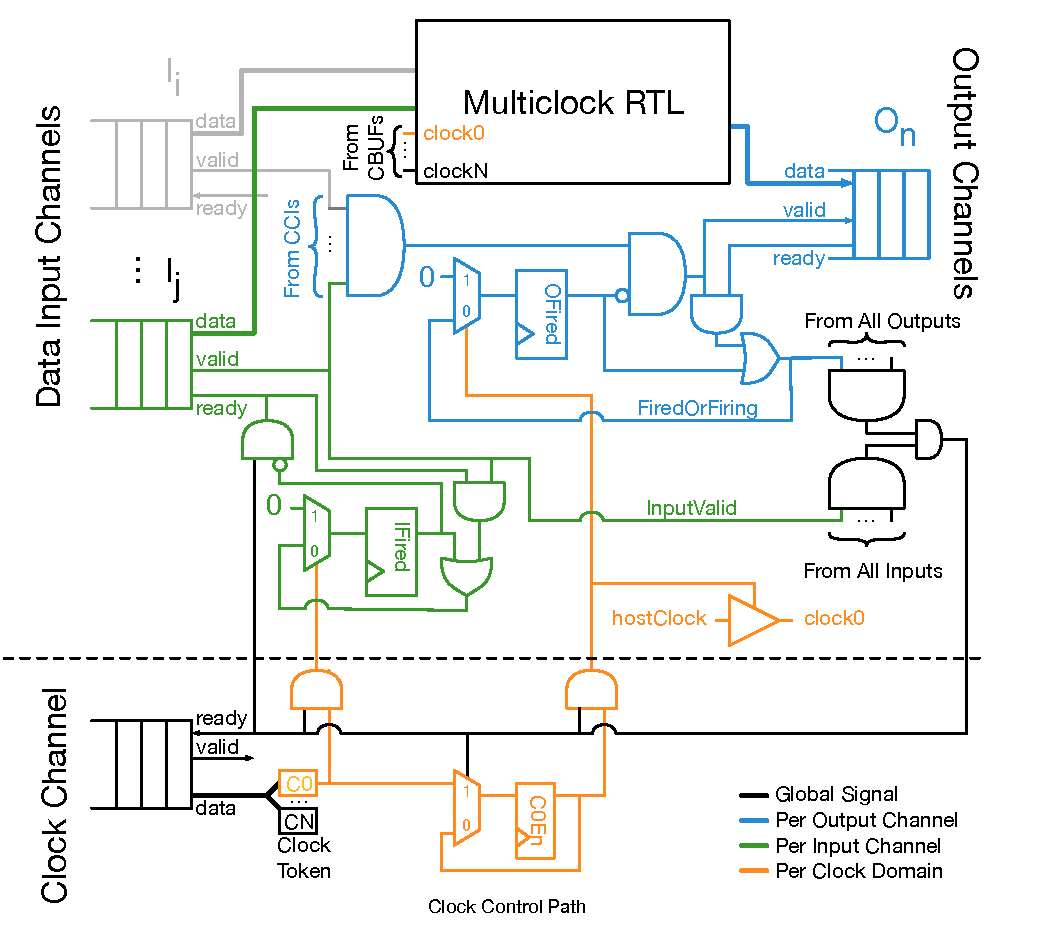
\includegraphics[width=0.99\textwidth]{figures/static-multiclock-wrapper.pdf}
    % graffle2pdf -c multiclock-wrapper midas-graphics/graffle/wrapper-transforms.graffle figures/static-multiclock-wrapper.pdf
    \caption{A wrapper-module-based conversion of multiclock target RTL with multiple clocks into a unit.}
    \label{fig:static-multiclock-wrapper}
\end{figure}

%\TODO{Is the extra register stage necessary?}

Initially all output FSMs are reset to zero, and the clock pipeline
register marked invalid (no clock is scheduled to fire).  This permits all combinational paths across all clock domains resolve based on the
initial input token values and target state.  As previously discussed, all
target clocks are gated under host reset such that BRAM and register state
initialized during FPGA programming cannot spuriously change as the FPGA comes
out of reset.

\subsection{Clock Bridge}

The clock bridge is responsible for determining the clock schedule by
generating an infinite token stream of $n$-wide bit-vectors, where $n$ is the
number of clock domains in the target. We show an example of this encoding for three rationally
related clocks in Figure~\ref{fig:clock-token}. Each clock token corresponds to a
simulator \emph{timestep}. Any clock with a positive edge in given timestep will have
its bit set in the corresponding clock token.

\begin{figure}
    \centering
    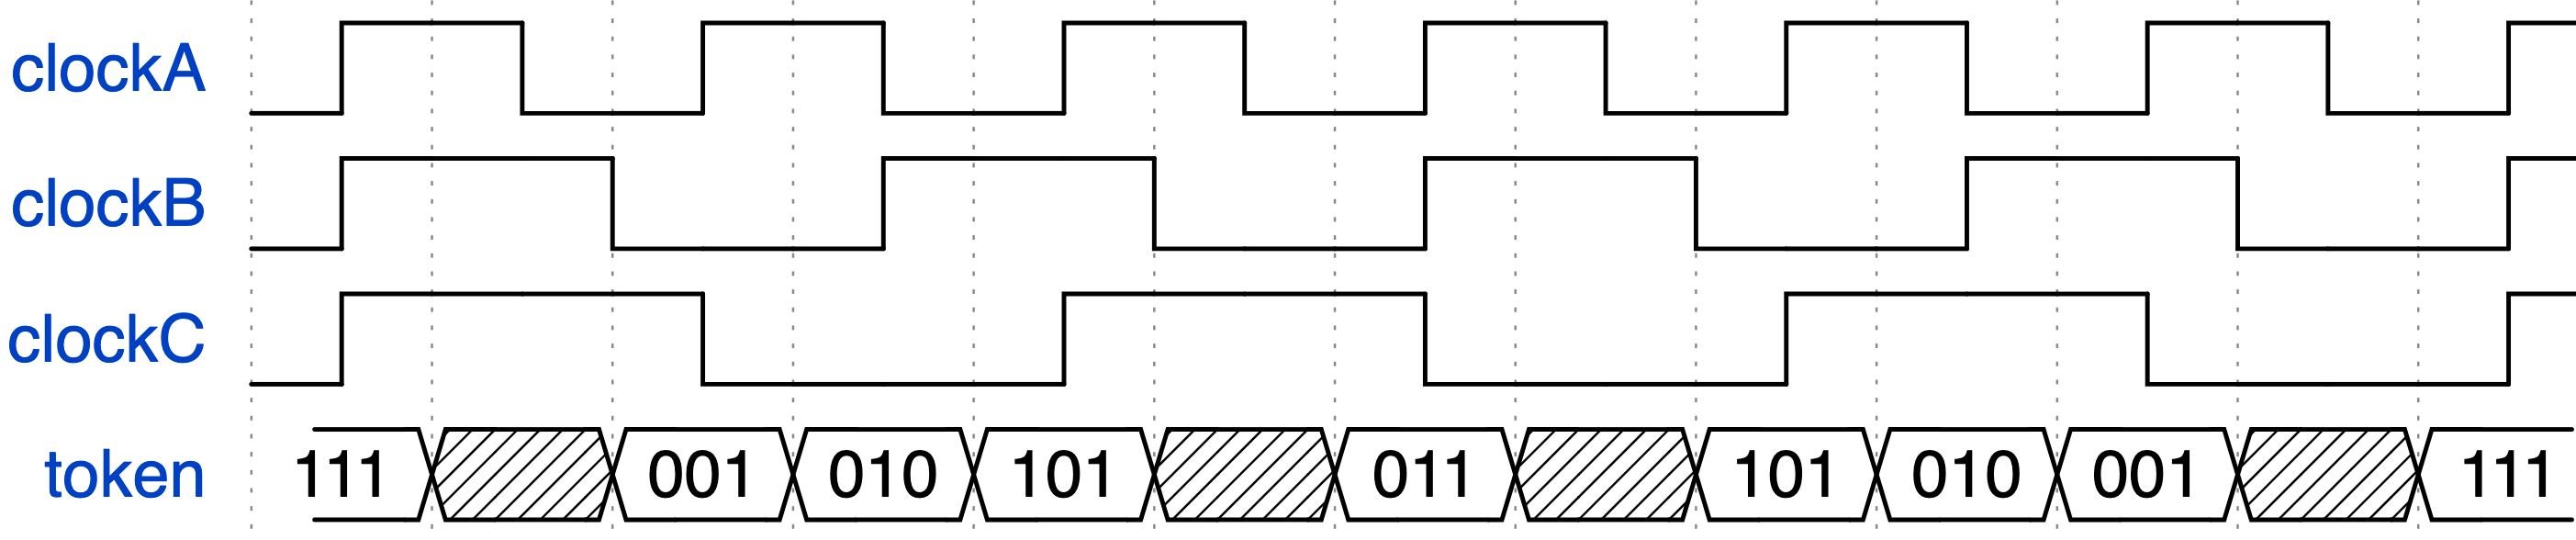
\includegraphics[width=\textwidth]{figures/clock-token.png}
    \caption{An example encoding of three rationally related clocks (clocks B and C have periods
    1.5 and 2 times longer than clock A) into a clock token stream. Here there is a recurrence
    after eight tokens, with the fastest clock active in all but two tokens.}
    \label{fig:clock-token}
\end{figure}

Per our earlier assumption, the clock bridge implementation included in FireSim 1.10 accepts clock specification that
defines the frequency of all clocks as rational multiple of the
frequency of the zeroth clock\footnote{Another reasonable approach would be to
specify the periods of all clocks in an agreed upon timebase. We note
that in this case all clocks are rationally related to a fast clock whose
period equals the resolution of the timebase.}. To model a clock that is not
rationally related (e.g., a periphery clock that generated by a
secondary PLL or is sourced from off-chip), the user should select a rational
multiple that would best match the desired frequency of the clock.  During
elaboration, the clock bridge determines a virtual fast clock from which all
output clocks can be derived via an integer division (in other words, it finds
a clocks whose frequency is the least common multiple of the frequency of the
requested clocks). Then for each output clock, it generates a series of
down counters (\texttt{timeToNextEdge}) which are systematically reset to the
division required to generate that output clock.

To generate an output token, the bridge does a min-reduction across each clock's
\texttt{timeToNextEdge} register, and broadcasts the result. All clocks whose
\texttt{timeToNextEdge} matches the minimum are scheduled clocks: their bit is
set in the output token, and their \texttt{timeToNextEdge} register is reset to
their division. Unscheduled clocks subtract the broadcasted time delta from
their registers, simulating the advance of time.  This implementation is
capable of producing a clock token with at least one bit set every host cycle.

\subsection{Other Compiler \& Bridge Modifications}

In our and our users' experience, bridges are difficult to write as they force
the developer to reason about both host and target-time considerations. To
prevent further exacerbating this problem, we elected to forbid bridges and
extracted models from having channels in multiple clock domains. This had three
primary implications:

\begin{enumerate}
\item User-instantiated bridges must explicitly indicate the clock to which
they are synchronous. Bridge-emitted channel annotations contain references to
this clock. This is a relatively trivial change, but one that affects user
facing code.

\item Debug synthesis passes must emit multiple bridges. For example, assertion
synthesis must generate a new bridge for each clock domain in which there is at
least one assertion. To do so, we built FIRRTL analyses to find source clocks
        by walking clock connectivity~(\texttt{FindClockSources}), and to group and wire
nodes (like an assertion condition) to the top-level based on each nodes source
clock(~\texttt{BridgeTopWiring}).

\item To populate extracted-model channels with references to clocks, we
introduced a transform (\texttt{FindDefaultClocks}, run before \texttt{ChannelExcision}) that analyzes top-level
clock connectivity between extracted models and the hub. Any stateful module
once extracted will have connection between a new clock output port on the hub
module and a sink port on the model. By
finding these connections, models can be labeled with a clock reference on the
hub model and their channels annotations can be subsequently updated.
\end{enumerate}

\subsection{The Base Clock}

In a target system with a single global clock it is natural to specify time
in cycles of that clock. Bridges can easily keep time with a counter that tracks the number of times it has fired. Introducing
multiple clocks complicates this: specifications of time must either be made
explicit, or specified in clock cycles of some agreed-upon common clock. In
either case, these specified times cannot be compared against a bridge-local
cycle counter without the local clock's frequency, or its relative frequency to
the agreed-upon common clock. This is problematic because many of FireSim's
features use specifications of global time. For example,
instrumentation bridges (e.g., assertion and print bridges) accept
runtime arguments that specify windows of time over which they should be
enabled. Since these features are implemented over multiple bridges in
multi-clock targets, clock domain information must be provided to each bridge
such that they can translate time specifications into local cycle counts.

Here we exploited out assumption that all clocks are rationally related and, in
order provide a user experience similar to the existing one, we elected to
specify times in cycles of the zeroth clock generated by the bridge. We refer
to this clock as the \emph{base clock}. In Chipyard 1.4, the clock bridge is
configured to make the fastest clock in the system its base clock, which in
practice, always drives the cores of the design.

To propagate information about a bridge's clock domain to its host-side
components, we added an analysis pass~(\texttt{TargetClockAnalysis}, which runs during target transformation)
 that determines the clock index for each bridge
by walking clock netlist back to the clock bridge's output port. Using that
index, the pass looks up the ratio of the bridge's clock relative to the base
clock. This is passed through the parameters instance to each bridge module
during platform mapping. Bridge modules typically serialize this information to the
simulation header so they can be used in the driver to recalculate times
specified in base-clock cycles in terms of their local clock.

\subsection{Rethinking Simulation Performance}\label{sec:multiclock-sim-perf}

In Section~\ref{sec:iron-law}. we described simple equations that govern
simulation performance.  Under a system with multiple clocks, these need to be
updated. Among our users FMR~(Equation \ref{eq:fmr}) is a popular abstraction, and sees frequent use
in conversations regarding simulation performance. Perhaps, the most natural
extension of FMR for multiclock contexts is to define it in terms of the fastest
target clock:

\begin{equation}
    FMR_{fastest} = \frac{cycles_{h}}{cycles_{t,fastest}}
\end{equation}\label{eq:fmr-fastest}

Henceforth, when referring to FMR in the context of multi-clock simulators we'll
be using $FMR_{fastest}$ unless otherwise stated.  Given our implementation,
when all other clocks in the target can be expressed as an integer divisions of
the fastest target clock (this target clock is the virtual fast clock), the
simulator can execute with unity FMR. However, this is often not the case, especially
when modeling device clocks. For example, in a two clock system where the
second clock has a frequency two thirds that of the base, the best-case FMR the
simulator can achieve is $\frac{4}{3}$. This occurs since every other slow clock edge will not be
coincident with a fast clock edge and thus will require a simulator timestep in which no fast clock edge is processed.
We show this effect in token stream illustrated in Figure~\ref{fig:clock-token}).

An alternate measure of simulator efficiency, one that reveals the presence of
host-time stalls independent of frequency selection, considers all host cycles in
which the hub model is firing at least one target clock. We define \emph{model
activity ratio}~(MAR):

\begin{equation}
    MAR = \frac{cycles_h}{timesteps}
\end{equation}\label{eq:mar}

Where timesteps is the number of host cycles in which one or more target
clock edges are launched, or in other words, the total number of clock tokens
consumed by the hub model. Like FMR, a larger MAR corresponds to worse
simulation performance, however, in the absence of other host-time stalls all
Golden Gate simulators can run at unity MAR.

%\section{Evaluation}

% Resource utilization?
%- Clock bridge resources, fmax?
%- Scale a full system over multiple clocks

\section{Case Study - SPEC CPU 2017 Integer Performance}\label{sec:spec-perf}

Armed with the capacity to simulate multiple clock domains natively, we can
quantify the performance difference between single clock designs and more
realistic multi-clock designs. For this experiment we used otherwise standard
Chipyard SoCs (their block diagrams match that shown in
Figure~\ref{fig:gg-target}) and modified the clock domain organization. For
simplicity, in all cases we coupled the periphery and uncore domains.
We considered three different configurations:

\begin{enumerate}
    \item A completely synchronous configuration running at 1.5 GHz. FASED DRAM timings were scaled up
        by approximately 1.5 times to match a DDR3-2133 speedgrade.
    \item A two-domain organization with the memory bus and backing DRAM subsystem sitting behind
        an asynchronous CDC. Here the memory bus runs at 1.0 GHz, and the rest of the system
        remains clocked at 1.5 GHz.
    \item A three-domain organization that loosely matches the Freedom
        Unleashed where tiles run at 1.5 GHz and the uncore runs at 750 MHz
        with a low-latency rational CDC between them. The DRAM memory
        system remains unchanged from the previous organization.
\end{enumerate}


\begin{table}[t]
\centering
    \begin{tabular}{c c c}
    \hline
        \textbf{Parameter} & \textbf{Rocket} & \textbf{SonicBOOM} \\
    \hline
        Machine Width & 1 & 5 issue, 3 commit\\
        ROB Depth & N/A & 96 \\
        %Branch Predictor & TODO & Tage \\
        L1 I\$ Capacity & 16 KiB & 32 KiB \\
        L1 I\$ Associativity & 4-way & 8-way \\
        L1 ITLB Capacity & 32 & 32 \\
        L1 D\$ Capacity & 16 KiB & 32 KiB \\
        L1 D\$ Associativity & 4-way & 8-way \\
        L1 DTLB Capacity & 32 & 16 \\
        L1 \& L2 Block Size & \multicolumn{2}{c}{64B} \\
        L2 TLB Capacity &  \multicolumn{2}{c}{1024} \\
        L2 Cache Capacity & \multicolumn{2}{c}{2 MiB}\\
        L2 Cache Associativity & \multicolumn{2}{c}{8-way}\\
        L2 Cache Banks & \multicolumn{2}{c}{4}\\
        System Bus Width & \multicolumn{2}{c}{128b}\\
        Memory Bus Width & \multicolumn{2}{c}{256b}\\
        DRAM Speedgrade & \multicolumn{2}{c}{DDR3-2133 (14-14-14-47)} \\
        Memory Access Scheduler & \multicolumn{2}{c}{FR-FCFS} \\
    \end{tabular}
    \caption{Microarchitectural parameters of the two targets under test. Note, that BOOM's L1 cache under the
    under the ``Large" preset is twice as large as Rocket's (32 vs 16 KiB).}
    \label{tbl:core-parameters}
\end{table}


For each of these three organizations, we studied SoCs based around two
fundamentally different pipeline microarchitectures: Rocket~\cite{RocketChip},
a 5-stage, in-order scalar core, and SonicBOOM~\cite{SonicBOOM}, the latest iteration of UCB-BAR's out-of-order
superscalar core. We used the preset ``Large" core configurations for
both microarchitectures: their parameters can be found in
Table~\ref{tbl:core-parameters}. Since BOOM can dynamically schedule around
hazards like load misses, it should be able to drive more
memory system bandwidth (it has 4 L1 data cache MSHRs) and tolerate additional
latency through the memory system. We kept the
uncore and DRAM memory system configurations, which consisted of a four-bank, 2
MiB L2 Cache and FASED-modeled, single-channel DDR3 memory system, fixed across
the two designs. Note, we are not using FASED's optional last-level-cache model,
but instead an ASIC-optimized design generated using SiFive's open-source cache generator~\cite{SiFiveCache}.

\begin{figure}[htb]
    \centering
    %\captionsetup{margin=0.25cm}
    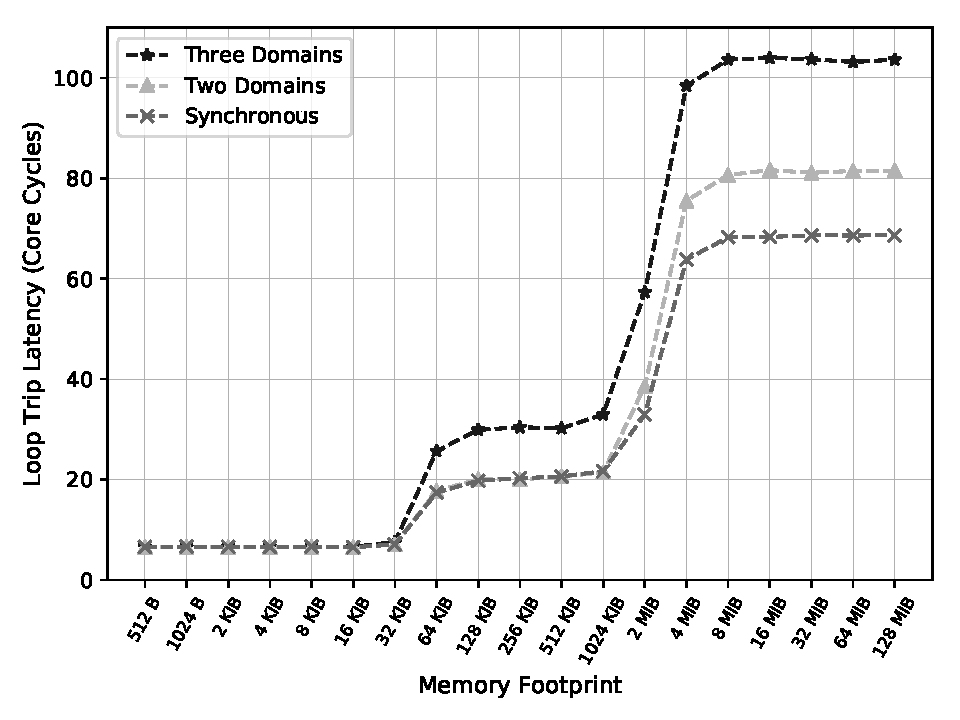
\includegraphics[width=\columnwidth]{figures/boom-ccbench.pdf}
    \caption{Execution latency, measured in core cycles, of one iteration of a randomized pointer chase
    for different array sizes (running on BOOM).
    }
    \label{fig:boom-ccbench}
\end{figure}

We used the ccbench~\cite{ccbench} ``caches" microbenchmark to measure round-trip latencies latencies
through the memory system under all three clock organizations. In
Figure~\ref{fig:boom-ccbench}, we show the loop trip latency when doing a
randomized pointer chase over different working set sizes running on BOOM (note, the pointer
chase touches each cache line only once). Marginal latency introduced in the
two-domain design over the synchronous design can be attributed to the addition of an asynchronous CDC
plus the additional latency introduced by register stages now running relatively
more slowly than the cores (these could not be trivially scaled by multiplying
a configurable value). Marginal latency introduced in three domain
configuration can be attributed solely to running the uncore clock at half rate.

\begin{table}[t]
\centering
    \begin{tabular}{c@{\hskip 0.1in} S[table-format=3.2] S[table-format=3.2] S[table-format=3.2]}
    \hline
        \textbf{Benchmarks} & \textbf{Insns~(T)} &\textbf{D\$ MPKI} & \textbf{I\$ MPKI} \\
    \hline
        600.perlbench\_s & 2.98 & 9.0 & 10.0 \\
        602.gcc\_s & 2.43 & 36.6 & 9.7 \\
        605.mcf\_s & 1.60 & 97.9 & 0.1 \\
        620.omnetpp\_s & 1.11 & 56.9 & 9.3 \\
        623.xalancbmk\_s & 1.21 & 62.9 & 7.9 \\
        625.x264\_s & 4.55 & 3.0 & 2.9 \\
        631.deepsjeng\_s & 2.51 & 8.7 & 15.4 \\
        641.leela\_s & 2.59 & 5.8& 1.5 \\
        648.exchange2\_s & 3.24 & 0.0  &  0.1 \\
        657.xz\_s & 9.41 & 19.8 & 0.2 \\
    \hline
    \end{tabular}
    \caption{Dynamic instruction counts and L1 MPKIs of SPEC2017 Integer Speed (single-threaded) benchmarks.}
    \label{tbl:spec-insns}
\end{table}

In this case study, we'll look at single-threaded performance of SPEC 2017
Integer Speed benchmark suite.  This suite has many of the same benchmarks as
its predecessor, the SPEC2006 suite used by Lee and Waterman in their VLSI
evaluation of FireSim, however each the benchmark's inputs are larger to better stress modern memory systems.
To provide some insight into the suite's memory system characteristics, in
Table~\ref{tbl:spec-insns} we report dynamic instruction counts,
and L1 cache misses-per-kilo-instruction (MPKIs) running on a Rocket configuration with the 
same L1 cache organization as the ones use in our study\footnote{These figures were
originally reported in our 2019 FASED publication.}.  We cross-compiled SPEC using Speckle~\cite{Speckle} and GCC version 9.2.0 with -O2
optimizations enabled.  We ran SPEC on top of simple Buildroot Linux
distributions we assembled using FireMarshal~\cite{FireMarshal}.  Our
system-software setup is reproducible without modification using FireSim
version 1.11 and Chipyard 1.4, following the instructions for building SPEC2017
provided in our documentation.

\begin{figure}[htb]
    \centering
    %\captionsetup{margin=0.25cm}
    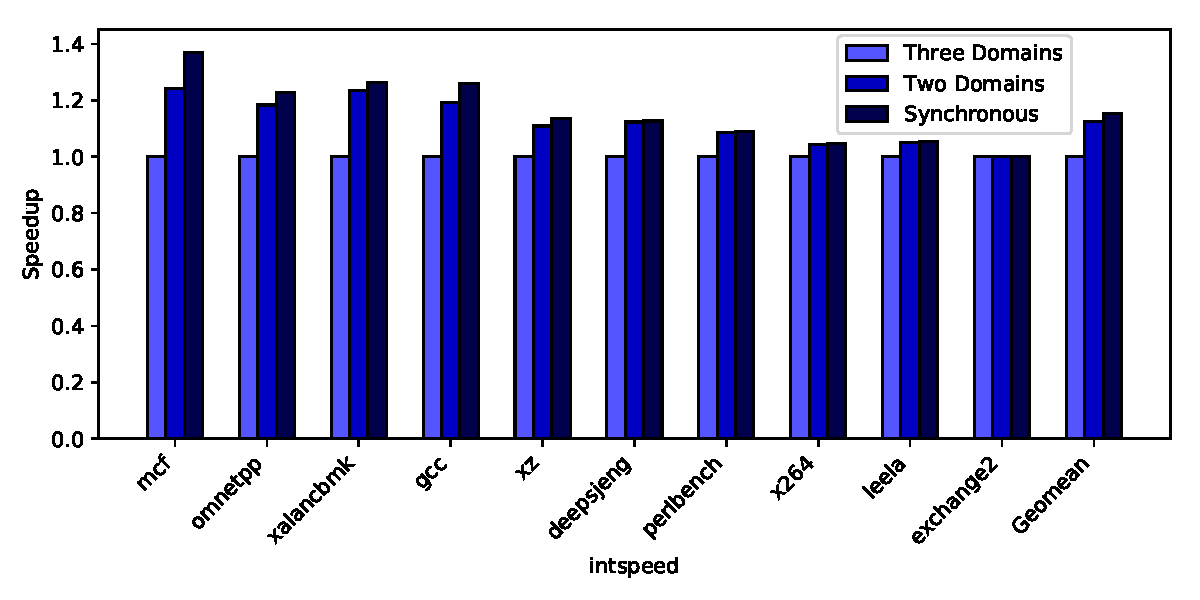
\includegraphics[width=\columnwidth]{figures/rocket-static-multiclock-speedup.pdf}
    \caption{SPEC 2017 Integer Speed performance on Rocket. Speedups are relative to the three-domain clock organization.
    Geomean speedups for the two domain and synchronous configurations are $1.12\times$ and $1.15\times$ respectively.}


    \label{fig:rocket-static-speedup}
\end{figure}
\begin{figure}[htb]
    \centering
        %\captionsetup{margin=0.25cm}
    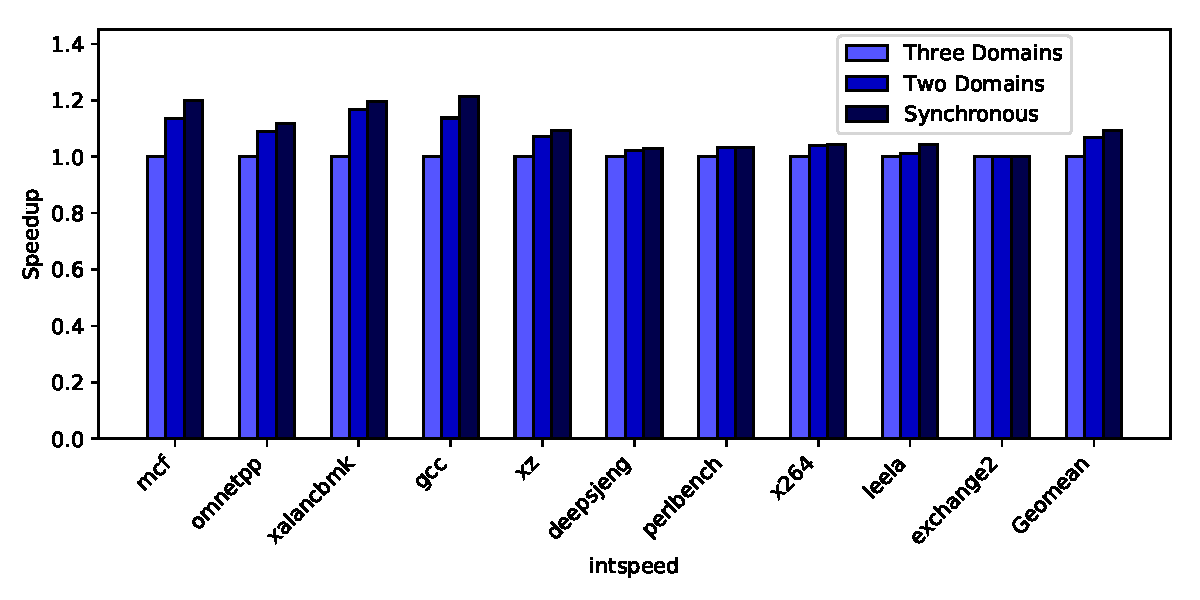
\includegraphics[width=\columnwidth]{figures/boom-static-multiclock-speedup.pdf}
    \caption{SPEC 2017 Integer Speed performance on BOOM. Speedups are relative to the three-domain clock organization.
    Geomean speedups for the two domain and synchronous configurations are $1.07\times$ and $1.09\times$ respectively.}
    \label{fig:boom-static-speedup}
\end{figure}


In Figure~\ref{fig:rocket-static-speedup} and Figure~\ref{fig:boom-static-speedup}, we report
SPEC runtimes as speedups relative to the most detailed three-domain
configuration. BOOM designs insulated themselves better from the additional
memory system latency brought about by running the outer memory systems at
slower frequencies, with synchronous designs running only $1.09\times$ faster
versus $1.15\times$ for Rocket based designs. While in Rocket's case, speedups
correlate closely with L1 cache MPKI, BOOM's ability to dynamically schedule
around these misses complicates the story. \texttt{605.mcf}, the benchmark with
the highest frequency of L1 data cache misses\footnote{This remains the case on
the BOOM configuration's larger 32 KiB L1 cache.}, runs $1.37\times$ faster on a synchronous Rocket
design vs $1.20\times$ on a BOOM design. Instead, BOOM sees its largest
performance change on \texttt{602.gcc} ($1.21\times$ versus $1.26\times$ for
Rocket), which reveals that core is able to find more ILP in \texttt{605.mcf}
despite having less data locality than \texttt{602.gcc}.

\begin{table}[t]
\centering
    \begin{tabular}{c
        S[table-format=2.0]@{\hskip 0.30in}S[table-format=3.0]@{\hskip 0.4in}
        S[table-format=2.0]@{\hskip 0.30in}S[table-format=3.0]@{\hskip 0.4in}
        S[table-format=2.0]@{\hskip 0.30in}S[table-format=3.0]@{\hskip 0.4in}
        S[table-format=2.0]@{\hskip 0.30in}S[table-format=3.0]@{\hskip 0.4in}
        S[table-format=2.0]@{\hskip 0.30in}S[table-format=3.0]
    }
\hline
         \multirow{2}{*}{\textbf{Target}} &
         \multicolumn{2}{c}{{\hskip -0.2in}\textbf{perlbench}} &
         \multicolumn{2}{c}{{\hskip -0.2in}\textbf{gcc}} &
         \multicolumn{2}{c}{{\hskip -0.2in}\textbf{mcf}} &
         \multicolumn{2}{c}{{\hskip -0.2in}\textbf{omnetpp}} &
         \multicolumn{2}{c}{{\hskip -0.2in}\textbf{xalancbmk}} \\
        &
        \multicolumn{1}{l}{{\hskip -0.00in}time} & \multicolumn{1}{l}{{\hskip -0.05in}$f_{emul}$} &
        \multicolumn{1}{l}{{\hskip -0.08in}time} & \multicolumn{1}{l}{{\hskip -0.05in}$f_{emul}$} &
        \multicolumn{1}{l}{{\hskip -0.08in}time} & \multicolumn{1}{l}{{\hskip -0.05in}$f_{emul}$} &
        \multicolumn{1}{l}{{\hskip -0.08in}time} & \multicolumn{1}{l}{{\hskip -0.05in}$f_{emul}$} &
        \multicolumn{1}{l}{{\hskip -0.08in}time} & \multicolumn{1}{l}{{\hskip -0.00in}$f_{emul}$} \\
\hline
BOOM-1D &      19.8 &   64.5 &  21.6 &  57.0 &  22.7 &  53.1 &    11.8 &   60.3 &       8.5 &   61.9 \\
%b2d &      26.4 &   48.6 &  28.2 &  46.6 &  28.3 &  44.9 &    15.5 &   47.3 &      11.3 &   47.9 \\
BOOM-3D &      29.5 &   44.9 &  34.4 &  43.4 &  34.4 &  42.1 &    18.1 &   43.9 &      14.2 &   44.4 \\
\hline
Rocket-1D &      14.2 &  108.9 &  19.8 &  94.9 &  28.0 &  87.8 &    10.8 &  103.5 &       9.0 &  103.9 \\
%r2d &      18.9 &   82.2 &  25.8 &  77.0 &  36.4 &  74.7 &    14.3 &   80.9 &      12.0 &   80.3 \\
Rocket-3D &      20.5 &   82.2 &  30.3 &  78.0 &  44.3 &  76.2 &    16.9 &   81.2 &      14.7 &   80.8 \\
\bottomrule
\end{tabular}
\vspace{0.5cm}

%\caption{First half}
%\end{table}
%
%\begin{table}[t]
    \begin{tabular}{c
        S[table-format=2.0]@{\hskip 0.30in}S[table-format=3.0]@{\hskip 0.4in}
        S[table-format=2.0]@{\hskip 0.30in}S[table-format=3.0]@{\hskip 0.4in}
        S[table-format=2.0]@{\hskip 0.30in}S[table-format=3.0]@{\hskip 0.4in}
        S[table-format=2.0]@{\hskip 0.30in}S[table-format=3.0]@{\hskip 0.4in}
        S[table-format=2.0]@{\hskip 0.30in}S[table-format=3.0]
    }
\hline
        \multirow{2}{*}{\textbf{Target}} &
         \multicolumn{2}{c}{{\hskip -0.2in}\textbf{x264}} &
         \multicolumn{2}{c}{{\hskip -0.2in}\textbf{deepsjeng}} &
         \multicolumn{2}{c}{{\hskip -0.2in}\textbf{leela}} &
         \multicolumn{2}{c}{{\hskip -0.2in}\textbf{exchange2}} &
         \multicolumn{2}{c}{{\hskip -0.2in}\textbf{xz}} \\
        & \multicolumn{1}{l}{{\hskip -0.00in}time} & \multicolumn{1}{l}{{\hskip -0.05in}$f_{emul}$} &
        \multicolumn{1}{l}{{\hskip -0.08in}time} & \multicolumn{1}{l}{{\hskip -0.05in}$f_{emul}$} &
        \multicolumn{1}{l}{{\hskip -0.08in}time} & \multicolumn{1}{l}{{\hskip -0.05in}$f_{emul}$} &
        \multicolumn{1}{l}{{\hskip -0.08in}time} & \multicolumn{1}{l}{{\hskip -0.05in}$f_{emul}$} &
        \multicolumn{1}{l}{{\hskip -0.08in}time} & \multicolumn{1}{l}{{\hskip -0.00in}$f_{emul}$} \\
\hline
BOOM-1D &       10.0 &   63.5 &       8.5 &   62.7 &   8.9 &   64.4 &       7.1 &   65.0 &  45.3 &   62.3 \\
%b2d &       13.3 &   48.1 &      11.3 &   47.7 &  12.2 &   48.5 &       9.5 &   48.7 &  59.9 &   48.0 \\
BOOM-3D &       15.0 &   44.4 &      12.5 &   44.2 &  13.4 &   44.8 &      10.3 &   45.0 &  69.3 &   44.4 \\
\hline
Rocket-1D &       14.7 &  108.4 &      10.7 &  109.0 &   9.5 &  109.5 &       9.7 &  109.9 &  47.8 &  107.2 \\
%r2d &       19.6 &   81.8 &      14.2 &   82.2 &  12.6 &   82.3 &      12.9 &   82.5 &  63.8 &   82.1 \\
Rocket-3D &       20.4 &   81.8 &      15.9 &   82.3 &  13.3 &   82.3 &      13.0 &   82.5 &  70.7 &   82.2 \\
\bottomrule
\end{tabular}

    \caption{SPEC 2017 Integer Speed (single-threaded) emulation performance.
    We report time~(wallclock) in hours, and $f_{emul}$, the effective
    emulation frequency of the cores of the design, in MHz. Note
    that \texttt{xz} had its inputs split over two emulators to approximately
    halve its runtime.}
    \label{tbl:spec-emulation-performance}
\end{table}


From an emulation performance perspective, simulating a more realistic clock
organization comes at the expense of increased runtime. As shown in
Table~\ref{tbl:spec-emulation-performance}, benchmarks take on average 49.4\%
and 53.0\% longer to simulate on the three-domain Rocket and Boom
configurations, respectively. The drivers of this are twofold. First, since
not all target clocks are integer divisions of the tile clock, simulation
performance is bound to a best-case FMR of 4/3~(due to the effect we described in
Section~\ref{sec:multiclock-sim-perf}). This caps $f_{emul}$ to 82.5 MHz and
45 MHz for the Rocket and BOOM-based designs, respectively. Second, the
multi-clock designs are simply slower target-designs thus will take more target clock
cycles to evaluate~(this is captured in Figure~\ref{fig:rocket-static-speedup}
and Figure~\ref{fig:boom-static-speedup}). These effects are offset modestly in
multi-clock
simulators by a reduced MAR: the host DRAM memory system has more time to serve
FASED requests leading to fewer memory-system induced stalls. This is reflected in memory intensive benchmarks like
\texttt{605.mcf}, where Rocket $f_{emul}$ runs at 93\% of the maximum 82.5
MHz~(MAR = 1.08), whereas the synchronous design achieves only 79 \% of 110 MHz
host frequency~(MAR = 1.49). Conversely, the runtime of benchmarks like
\texttt{648.exchange2}, which run completely out of cache and thus have unity MAR, are
completely exposed to the $\frac{3}{4}\times$ slowdown brought about by the clock-token
stream. Finally, in a testament to recent BOOM microarchitectural improvements,
the BOOM-based experiments took less time to run than the equivalent Rocket
configurations despite having average $f_{emul}$s of roughly half that of
Rocket's.

The times we report in Table~\ref{tbl:spec-emulation-performance} are directly
proportional to the cost of running the benchmark on AWS. At time of writing,
EC2 F1 2x.large instances cost \$1.65/hr for on demand instances, and \$0.50/hr
(typically) for spot instances. Considering just the BOOM designs, total
emulation time was 164 and 251 hours for the synchronous and three-domain
designs, respectively: on the spot these experiments would cost \$82 and \$126. One
implication of AWS's cost model is that there no disincentive to
using more FPGAs to improve simulation throughput. While
Table~\ref{tbl:spec-emulation-performance} reports an enormous runtime for
\texttt{657.xz}, this is the sum of its two roughly balanced inputs, so we split the
benchmark into two parallel runs to better balance the runtime of the
suite\footnote{Note, this is more difficult to achieve using the SPEC-provided
\texttt{runcpu} utility. In these experiments we are directly invoking the
benchmark binaries using Speckle-generated scripts.}. All told, \texttt{605.mcf} is the longest running benchmark on Rocket
(28.0 h and 44.3 h) versus the CPU2006docs input of \texttt{657.xz} on BOOM (23.4 h
and 35.8 h).

\section{Scaling Target Clock Count}\label{sec:clock-scalability}

For targets with relatively few clock domains, Vivado is generally able to
successfully place and route without any additional placement constraints.
Though clock routing and distribution was enhanced in Xilinx's Ultrascale
architecture, global clock resources are still scarce relative to conventional
logic interconnect. More concretely, designs that require more than 24 global
clock nets be routed through the same clock region will fail in implementation.

To establish a baseline for the scalability of our approach, we attempted to synthesize a
toy target design consisting a shift register with each of its stages driven by a different clock. 
Thus for an $N$ stage shift register, $N$ BUFGCEs will be
instantiated in the hub model. Since each stage is small, this is an adversarial
design: Vivado will attempt to place all registers in the same clocking region
(to reduce path delay), only to discover it has insufficient clocking
resources to drive the sinks. Using Vivado 2018.3 and FireSim's custom AWS shell (based off version 1.4.8), we found that we could synthesize a 12-stage
pipeline before running out of global clock resources in at least one clock
region. In this region only 13 of 24 available nets are used for the implementation of
the hub model: the remaining 11 are used to route clocks for IP blocks like DDR
controllers and PCI-E, which are periodically striped down the FPGA. Excluding
the clocks used in Golden Gate-generated RTL, median global clock-net
utilization across the device is 11 (ranging between 9 and 23) across the 90
available clock regions of our VU9P part. This will prove problematic for simulating systems
with dozens of clocks, which is not unheard of in modern SoCs.

We propose two means to attack this challenge. The first is obvious and follows Xilinx's recommendation:
minimize the number of unique clocks required in each clock region by
preventing placement of too many distinct clock domains. This may occur naturally
if, unlike the design above, each clock domain has significantly more logic.
During placement domains will tend to exclude each other as the placer will
tend to put primitives in the same clock domain closer together. Alternatively,
it may be possible to optimize the AWS shell to reduce the number of global
clock resources it requires, or better isolate its clock domains from the rest
of the simulator's. In worst case, however, placement constraints on parts of
the hub unit may be required.

A second approach may be to save global clock resources by converting a gated
clock to use a clock enable, which can be driven through logic interconnect.
This introduces a high fanout logic net but for relatively small clock domains could save global clock resources
by reusing the ungated host clock~(if it is being routed to the
clock region already). This optimization could be implemented by Golden Gate
without user intervention.

\section{Improving Simulator Performance with Multi-Cycle Setup Constraints}\label{sec:multi-cycle-constraints}

On the surface, one challenge with using a single host clock is that all
paths in the target must close timing at the emulator frequency.
In effect, Vivado will use the same setup relationship to close timing on paths
whose delays are many times longer than that of critical path in the fastest
clock domain. FPGA prototypes avoid this problem entirely since each
domain is driven with clocks of the same relative frequency as would exist on the SoC, giving slower clock domains
more setup margin. When this is combined with the fact that out-of-phase
edges in slower domains can be launched between fast-clock edges, FPGA
prototypes have a considerable performance advantage over the equivalent
multi-clock FireSim emulator.

One way to close this gap is to improve $f_{fpga}$ by giving Vivado more
setup margin on paths in slower target-clock domains. Here we exploit the
observation that, given our current clock-token generation scheme, clocks in
all but the fastest target-clock domain cannot have positive edges launched in
back-to-back host clock periods. This implies that data launched in one domain
will not be captured by state elements in the same domain until at least two
host cycles later. We can indicate this to Vivado using a multi-cycle setup
constraint on all timing arcs that are internal to that domain. In many cases
this setup relationship can be larger than two periods. A clock that has a frequency one $n^{th}$ that
of the fastest clock, can be given a setup constraint of $n$ periods.
Additionally, the presence of other clocks with frequencies that are not
integer divisions of the fastest clock can further lengthen this constraint.
Since the clock token stream is known at compile time, Golden Gate can analyze
these relationships and emit target-specific multi-cycle constraints.  In
principle, similar constraints could be emitted for inter-clock-domain paths,
but this would require the presence of intermediate clock-tokens between the
positive edges of both domain clocks.

To illustrate the potential of these relaxations, we manually applied a
two-cycle setup constraint to all intra-domain paths in the DRAM and uncore
domains for the three-domain targets we evaluated in
Section~\ref{sec:spec-perf}. We then resynthesized both sets of
designs, with the constraints and without, using overconstrained host
frequencies to establish an emulator $f_{max}$. We report the improved
simulator frequencies in Table~\ref{tbl:multi-cycle-constraints}. The Rocket
based design saw greater improvements than BOOM for a few potential reasons.
Firstly, in an ASIC technology, Rocket can be realized at higher frequencies than
BOOM. Second, delays
through common structures in OoO microarchitectures scale more poorly when
mapped to FPGAs relative to in-order designs which lack many of the same
structures. Taken together, the ratio of core path-delay to uncore path-delay
is closer to parity in BOOM, than in the Rocket-based design where it is closer
to the expected one-to-two ratio one would realize in the equivalent ASIC.

\begin{table}[t]
\centering
    \begin{tabular}{c@{\hskip 0.1in} S[table-format=3.1] S[table-format=3.1] S[table-format=3.1]}
    \hline
        \textbf{Design} & \textbf{Unrelaxed $f_{max}$} & \textbf{Relaxed $f_{fmax}$} & \textbf{\% Difference} \\
    \hline
        Quad-Core Rocket & 112.5 & 168.1 & 49.4 \% \\
        Single-Core Large Boom & 70.5 & 90.0 & 28.5 \% \\
    \hline
    \end{tabular}
    \caption{Simulator $f_{max}$ for the designs of the SPEC performance
    study without (\emph{Unrelaxed}) and with~(\emph{Relaxed}) multi-cycle
    setup constraints applied.}
    \label{tbl:multi-cycle-constraints}
\end{table}

One consequence of increasing $f_{fpga}$ is that various extra-emulator domain
delays will now appear to have greater latency (e.g., FASED's host DRAM
requests will take more cycles to be served), which could increase FMR. To
provide some perspective on this effect, we booted linux on instances of the
relaxed and original designs that passed timing~(we used the same simulators from the SPEC performance experiment).  We report the change in
simulation performance in Table~\ref{tbl:multi-cycle-constraints-perf}. Linux
boot differs from SPEC in that has periods of sustained disk and DRAM use and
so tends to have a greater FMR. While FMR does increase in the relaxed
simulators it only modestly reduces the improvement brought about by the
increased $f_{fpga}$. Were we to re-run the SPEC performance study from
Section~\ref{sec:spec-perf}. we estimate the multiclock designs would take
roughly as long to simulate as the synchronous ones, permitting a SPEC run to
complete in approximately a day.

\begin{table}[t]
\centering
    \begin{tabular}{c@{\hskip 0.4in} S[table-format=3.0] S[table-format=1.2] S[table-format=3.1]@{\hskip 0.3in}
        S[table-format=3.0] S[table-format=1.2] S[table-format=3.1]@{\hskip 0.3in} S[table-format=1.2]}
    \hline
        \multirow{2}{*}{\textbf{Design}} & \multicolumn{3}{c}{{\hskip -0.3 in}\textbf{Unrelaxed}} & \multicolumn{3}{c}{{\hskip -0.3 in}\textbf{Relaxed}} &  \\
        & $f_{fpga}$ & FMR & $f_{emul}$ & $f_{fpga}$ & FMR & $f_{emul}$ & {Speedup} \\
    \hline
        Quad-Core Rocket & 110 &  1.45 & 76.0 & 150 & 1.49 & 107.3 & {$1.41\times$} \\
        Single-Core LargeBoom & 60 & 1.57 & 38.2 & 90 & 1.65 & 54.5 & {$1.43\times$} \\
    \hline
    \end{tabular} \caption{Simulator $f_{max}$ for the designs of the SPEC
    performance study without (\emph{Unrelaxed}) and with~(\emph{Relaxed})
    multi-cycle setup constraints applied. Note, the BOOM result is arguably
    optimistic since the unrelaxed variant still has a fair amount of setup
    margin under a good initial placement.}
    \label{tbl:multi-cycle-constraints-perf}
\end{table}

\section{Future Work}

The support for multiple clock domains described in this chapter and released
in FireSim 1.10 is an important development over previous iterations of the
compiler, as it eliminates a key barrier to doing realistic pre-silicon
performance validation.  Within the assumptions laid out in
Section~\ref{sec:static-multiclock-assumptions}, there are still a number of
improvements we could explore.

\begin{enumerate}
    \item  \textbf{Automatic generation of target-specific, multi-cycle setup constraints.} As we
showed for a limited set of designs in
Section~\ref{sec:multi-cycle-constraints}, multi-cycle setup constraints can
provide an enormous performance benefit. In future, we plan to have Golden Gate emit target-tailored
constraints these during compilation so these benefits are automatically passed
on to the user.

\item \textbf{Improve best-case FMR by combining clock tokens}. Here we exploit the observation that if the state
updates brought about clock token $N$ are not observable by any domain
scheduled to fire in clock token $N+1$, it is safe to fuse these two tokens
into single token with the union of their bits set. In many cases, this will
address the performance cost described in
Section~\ref{sec:multiclock-sim-perf}. In that example, clock tokens that fire
only the DRAM clock can be fused into prior tokens that fire only the tile clock,
and vice versa. This would restore the best-case FMR to 1, since all
tokens would carry a tile clock edge. However, this optimization does not come without cost. First, it complicates any debug utility that wants to observe target
state at time between the edges scheduled in fused token. Second, it may
preclude applying the multi-cycle setup constraints described above to some
domains~(in our example, the DRAM domain now fires in back-to-back host cycles),
potentially offsetting some of the benefit of the optimization. From an
implementation perspective, producing a simplified connectivity graph that
could be fed into the clock bridge generator is relatively straightforward
process in FIRRTL and so this optimization can be easily explored.

\item \textbf{Investigate schemes for improving clock scalability.}
Firstly, we need to better understand the scaling trends for different targets
and different Vivado implementation strategies.  In
Section~\ref{sec:clock-scalability} we proposed two means to improve
the number of clocks we can simulate in a single target. Automatic
gated-clock conversion is a relatively straightforward optimization as
in FIRRTL we can easily assess
the number of clock loads in a domain and selectively emit clock-enables
instead of a BUFGCE---this is no different than how MIDAS's FAME-1 transformation
implemented SSM to patient-SSM conversion. Providing placement constraints
would be effective solution, although trying to automatically emit them brings to mind many of the
challenges that plague automatic floorplanning. In lieu of that, providing a user-friendly mechanism to
provide customized placement constraints would be a very useful intermediate
step.

\item \textbf{Runtime-configurable target clock frequencies.} To avoid needing to
synthesize multiple bitstreams to evaluate different clock frequency
selections, we could make the rational relationships encoded in the clock bridge runtime programmable.
Note, the number of clocks and target clock-crossing circuitry would remain
fixed, which limits the utility of this feature. From an implementation perspective, this feature would require propagating
clock domain information to relevant bridges at runtime instead of at compile time,
but otherwise this feature is straightforward to implement.
\end{enumerate}

Ultimately, some of the assumptions we outlined in
Section~\ref{sec:static-multiclock-assumptions}, could be relaxed without a
large scale reimplementation. For instance, the clock bridge can easily be
modified to generate tokens for any clock whose edge times are known \emph{a priori}.
Lifting effectively \emph{all} of these constraints, most notably to
support dynamically changing clock frequencies, is a more challenging
undertaking that requires a rethinking of clock bridge abstraction. This is the
subject of the next, and final, chapter of this dissertation.



\chapter{Modeling Asynchrony with Explicit Timestamping}\label{sec:dynamic-multiclock}

% High level idea:
% Introduce timestamped units into the simulator graph, existing models remain implicitly timestamped.

The fundamental assumption made in the previous chapter was that the clocks of
the target cannot change as a function of the simulated behavior of the target
itself. This permits generating a clock-token stream that can runahead of the
rest of the simulator and gives good simulation performance. Lifting this
assumption introduces a potentially performance critical feedback loop into the
emulator: scheduled clocks determine when target state updates occur, but those
updates themselves affect when target clocks are scheduled.
% We illustrate this with a simple example\TODO(clock mux).

Academic work in this domain is lacking. The only hardware-accelerated platform
for studying platforms that can preform DVFS was built by Mantovani et
al.~\cite{DVFSPrototype}. However, that work is essentially a configurable FPGA
prototype: it presupposes a particular target organization~(a grid of tiles
innerconnect with a NoC) and directly directly instantiates FPGA specific
clocking primitives. Using FPGA clocking primitives directly skirts preformance
challenge we outlined above, allowing their system to run fast (100 MHz on a
Virtex 7 FPGA). This makes it an attractive platform to do research on new
DVFS policies, but not generally useful for doing pre-silicon verification or
performance validation of an SoC which does not derive from their input RTL.

For examples of FPGA-based hardware emulation of systems that support dynamic
frequency scaling, one must look to industry. Mentor Veloce and Synopsys ZeBu,
both have support for systems that do this sort of frequency scaling --- how
they support this is propertiary. One 2013 Mentor Graphics patent provides some
insight as to how this may be implemented in Veloce: a compiler detects
``clock-enabling" functions in the target circuit, which are in-essence,
combinational logic functions that permit a clock to be driven to a particular
output node. For instance, the and-gate of a clock gate would be such a
function, controlled by a "clock-enabling single" the output of the latch. More
complex circuits, like clock multiplexers, can be decomposed into exclusive
sets of these enabling functions. These functions are combined into a single
``clock status" signal which indicate to the emulation clock generator that it
should drive a clock into the sink domain. Many critical details in this system
are intentionally left vague, and context related to emulator clock generation
is omitted.  What appears to be the case is that target behavior governing
clock selection and generation is managed at combinational level, which is a
sensible design decision for generalizing support for a broad range of targets.
It does seem to tightly couple clock generation and to target logic simulation.
One intriguing omission is the lack fine-grained timestamping , which in
conjuction with the observation above, seems to suggest some sort of
centralized control with minimal decoupling acrossing the emulator.

The approach we outline in this chapter is radically different than those
outlined above, in that clock generation and selection circuits are replaced
with indepedent decoupled units that are timestamped. In effect, this sub-graph
combined with the hub unit are a conservative PDES, and the resulting simulator
is ETDC.  In our implementation, no FPGA specific clock selection logic beyond
a clock gate, is used, making our implementation portable across different
FPGAs. In also maps well to inherently parallel nature of clock generation and
selection in a SoC. However, this implementation strategy begets its own
challenges however, notably the classic conservative PDES challenge achieving
good performance and avoiding deadlock hinges on finding sufficient lookahead,
which in some cases may not be possible without restricting target behavior.

\section{Context, Goals and Motivation}

To understand how we arrived at our implementation, we need to re-evaluate the
goals outlined when we designed Golden Gate. Understand the current capability
of FIRRTL to express clocking primitives, and the machinery available in Golden
Gate to implement these features. Re-evaluating the goals we laid out in
Section~\ref{sec:gg-design-objectives}.

\begin{enumerate}
\item \textbf{Maintain FireSim feature completeness.} Just as in the orginal
redesign, it was critical that support for dynamic frequency scaling, work in
conjunction with existing Bridges and multi-cycle resource optimizations. For
the purposes of getting to a working prototype, we will accept a loss of
simulation FMR. In the long run however, our goal is to support siulating
systems that dynamically change their clocks at the same rate as an equivalent
system that does not.

\item \textbf{Minimize user modification of ASIC RTL.}
Specifically, we want to avoid extensive changes to the designs module
hierarchy. The use of a singleton clock bridge in the previous chapter,
violated this objective. Indeed, in Chipyard 1.4, multi-clock configurations
are handled different in RTL simulation (where a high frequency clock source
drives multiple clock dividers), versus the FireSim configuration, in which all
of this is ripped out and replaced with an instantion of the clock bridge
outside the chip. For the purposes of this disseration, we'll permit replacing
ASIC clock-generating circuits with models that do not exactly the same behavior\TODO{Define this?}.

\item \textbf{Provide a mechanism to rigorously verify the [modifications].} We
decided to punt on this objective here. Though, as in LI-BDN case, it would be
nice in the future if replaced models could be verified against the underlying
ASIC implementation. In this chapter we relied on dynamic verification, but a
re-imaging of LI-BDN for asynchronous circuits is a long term goal.

\item \textbf{Enable the use of FireSim as a library for hardware emulation.}
This is closely related to teh second point. Clocking and reset structures
remain the single largest point of divergence between ``Chip" configurations and
FireSim configurations of Chipyard SoCs. At time of writing FireSim is being
used as a library outside of Chipyard, really, our aim is to support emulation
of arbitrary, but appropriately annotated, firrtl and not strictly Chipyard
designs.

\item \textbf{Avoid use of FPGA-specific Clocking Primitives.}
In the interest of supporting other FPGAs in the future, and to avoid more of
the placement and DRC challenges associated with using those devices, we wanted
a design that used coventional logic and interconnect resources where possible.
\end{enumerate}

Another important reality to grasp is that native support for clocking
structures in FIRRTL is nascent, and designers tend to use black-box verilog to
describe structures like clock gates and logic primitives that act on
clocks~(this have particular process-specific implementations that will be used
in physical design). As a result, buiding a compiler capable of analyzing this
netlist without conserable designer help was going to be intractable. Users will
need to provide this compiler-required information with FIRRTL annotations.

\section{Designs We Considered}

%For many of the same reasons descrbed the previous chapter, an
%FPGA-prototyping-based approaches like the one described by Mantovani et
%al.~\cite{DVFSPrototype} was off the table.

To resuse most of our work in building out static multiclock support, we
initially tried to frame dynamic clock domain support as solving the smaller
problem of reconstituting the clock-token stream. The most straightforward way
of doing so is to a provide a means for users to specify that certain clocks
have dynamic behavior on the centralized clock bridge. For these clocks, the
clock bridge would accept a parameters to describe how it derives from other
clock in the system (e.g., it should in effect simulate a clock mux and select
between two other output clocks). Based on this selected behavior a set of
target-drive inputs on the bridge would be exposed, and the user would drive
these from the target. This would require the least modification to existing
infrastructure as clock-enabling signals driven is already provided by bridge
extraction. This reverse channel could enqueue a new output token on each
simulator timestep, which in turn, may determine the contents of future clock
tokens.

While this would suffice for simulating simple systems, and would be easy to
implement initially, the main problem with this approach is that it forces the
designer to reexpress, in a centralized fashion, how all clocks in a system are
generated. The difficulty is that clock generation and distribution in an SoC
is a distributed process.  In a simple system, a clock source might feed a centralized PLL,
which in turn, drive a series of output dividers, downstream clock muxes and
clock gates, may be distributed throughout the design hierarchy. This simplified model is complicated by I/O
devices which tend their own clock generation schemes. As such, it would be
better if information about target clocks could be captured or inferred at the instantion
sites of the ASIC circuits that are responsible for generating derived clock in
the actual implementation, instead of forcing the user to rexpress these
properties at the clock bridge.

Indeed, in order to minimize modification to ASIC RTL it would be better to transform or
replace ASIC circuits with FPGA-compatible equivalents. As in the previous
chapter, this cannot be achieved simply by replacing a primitive with an FPGA
analog, but instead requires a host-decoupled unit that deterministically
models the behavior of the target circuit under variable host-timings.  While
tranforming verilog models of clock-generating circuits into an exact but
latency-insenstive equivalent (a la LI-BDN and SSMs) is a possibility in the
future, in this chapter we are going to substitute these circuits for
handwritten units. Golden Gate has extensive support for doing module-level
manipulations of the design hierarchy.  Instead of using this machinery to
preform resource optimizations, here we will leverage it extract and replace
clock generating circuits with equivalent units.

Of course, a unit, with the exception of the hub unit, represent SSMs with
tokens of a unit being synchronous to the clock of the SSM. This clearly does
not apply to clock generating circuits, whose inputs and outputs are
clocks, often without phase relation to one another. Here, some timekeeping can
no longer remain implicit: the times of each edge must be known to propely
model the underlying circuit.

Perhaps the defining of this project was whether to leave these
clock-generating circuits as independent units or whether the
compiler should attempt to centralize them into a single chunk of logic that could
feed the front-end of the hub (i.e., by subsuming the role of the clock bridge
and supplying complete clock tokens). In effect this is just a question of
centralized versus distributed control.  In the prototype we described in this
chapter, we elected to leave them as independent units, for the following
reasons:

- Naturally fit into the Golden Gate framework.
 - Of replacing modules with decoupled units.
- Can model a wide space of simulated behaviors. Complex behavior can be modelled in the replaced units. (See stanford).
  This behavrios can be reasonable about independently of other blcoks in the system. 
- Is a more interesting/unique system to study.

A time of writing, it remains unclear if this is a better solution, as it comes
introduces deadlock risks not associated with a centralized approach, and
relies extensively on finding adequate lookahead to achieve good performance.
Conversely, munging this logic together and coupling it directly to hub is
likely to work in a broader set of cases, and produce acceptable
performance---the final result would look much like Cadence patent described
previously.  We will speculatively explore this tradeoff at the end of this
chapter when we discuss future work.


\section{Initial Implementation}

As we have alluded to the previous section, our approach functions by replacing
modules related to clock generation, switching, or gating, or behaviors that
are otherwise asynchronous to a clock, with timestamped units~(an LP in PDES
parlance). This modules are extracted and replaced in the same fashion as a
Bridge or an optimized model, however, their channels are labelled as
``timestamped". Timestamped channels send, in PDES paralance, \emph{messages}:
a tuple of a data-value and a timestamp. Here, the resultings simulator graph
consists of an untimestamped subgraph, consisting of optimized models and
coventional bridges. and a timestamped subraph consisting of the timestamped
models. The hub-unit is the only unit that exists in both subgraphs, it has
both timestamped and unstamped input and output channels. We show an example graph in \TODO{Figure}.

To improve FMR on combinationally connected paths between units (timestamped or
unstamped), we introduced a compiler optimization that removes passthrough
connectivity in the hub. This permits two models to drive each other directly,
instead of passing through the hub model. As a result, simulator graphs are not
always stars (this is reflected in \TODO{Figure}). This optimization is
critical for improving FMR in non-trival timestamped, but as a side-effect, can
also improve FMR when multiple optimizations are enabled byt allowing
optimization models to drive each other directly. We expand on this in compiler modifications in \TODO{Section}.

Since there is no longer a single clock token stream, we modified the hub unit
to schedule across its multiple timestamped inputs. Timestamped inputs can be
either clock-type or data-type~(used for modelling asynchronous resets), these
differ in how they are presented to target RTL. The hub unit explicitly tracks
target time, which it uses to annotate timestamped outputs as the hub advances.
We expand on the hub-unit modifications in \TODO{Section}.

Easily the challenging aspect of this implementation was modelling
timestamped hardware. Timestamped units are implemented as bridges that use
timestamped channels exclusively. We wrote a chisel library to make it easy to
write simple models as translations of verilog RTL, allowing us to build models
quickly. These models are pessimistic, and do not exploit lookahead that might
be present in a larger circuit. To improve simulation performance, we explored
writing specialized models that extract multi-cycle lookahead that is available
in certain circuits.


% Show an example graph.
% - Two sides, time-stamped models on one side, existing LI-BDN models on the other
% Show a promote passthrough paths variant.

\subsection{Hub Unit Modifications}
% Hub model modifications.
% - Clocks
% - Async Reset

\subsection{Compiler Modifications}
% Baseline Compiler modifications
% - Extract passthroughs.
%   - Clock source + clock divider

\subsection{Baseline Timestamped Models}
% Library for building timestamped bridges
% - Dynamic verification of TS bridges
% - 2:1 Clock Mux Example

\section{Example Case Study}
% Baseline Performance & Resource Utilization
% Example designs: Parallel dividers cascade, parallel muxes, mux cascade, clock gate


\section{Performance Optimizations}
% Optimizations
% - Double tokens
% - Muxes with lookahead

\section{Deadlock Considerations}

% Full-system demo

\section{Future Work}
% - Optimized clock-muxes


%Patents:
%https://patents.google.com/patent/US20150046144A1/en
%


%\chapter{Conclusion}
%
%%Our goal in building out the FireSim project was to build a radically
inexpensive, yet fast and productive, cycle-accurate full-system simulation
technology to attack a key contributor to the NRE of building silicon.  While
our system is most similar to existing hardware emulators, our approach is
unique in that is uses a single COTS FPGA, and depends on a completely open
source toolchain. However, it was difficult to make this comparison in good
faith, as early versions of FireSim had two critical limitations: were limited
to supporting to small, single-clock domain.

We designed Golden Gate to address these limitations~(Chapter~\ref{sec:golden-gate}). First, Golden Gate uses a LI-BDN
target formalism and RAMP-inspired multi-cycle optimizations to fit larger SoCs
on a single FPGA; descriptions of these optimizations can be found in Albert
Magyar's dissertation. Overcoming the clocking limitations was the primary focus of this dissertation.
To model multiple clock domains, we introduced a new FAME transform that avoid
using dedicated FPGA clock resources like prior academic work, in favor of a
clock-gating scheme that should be portable to many different FPGA
platforms~(Chapter~\ref{sec:static-multiclock}.  To model clock switching an
generation circuits, which form the basis of dynamic frequency scaling support
in realistic SoCs, we introduced a timestamped subgraph into the simulator that
implements a conservative PDES~(Chapter~\ref{sec:dynamic-multiclock}).

One takeaway from our work in supporting clock switching and generation
structures is that closely coupled clock-generating circuits, like ICGs and
clock multiplexors, are probably best simulated \emph{in situ}, instead of
being extracted into a decoupled unit. State for these circuits can be left in
the target, and combinational functions they perform on clocks can be hoisted
into the hub-unit's second stage to act on future clock enables. This would
generate new clock buffers for these derived clocks. This clearly would be
insufficient for modelling clock generators like PLLs that can't be described
as digital functions on existing clocks, like PLLs.  For modelling this class
of circuits, having an independent TU unit seems entirely sensible.  This
hybrid approach would also reduce the number of timestamped inputs on the hub
unit, addressing a potential scalability challenge in systems with many clocks.
Implementing and studying this approach is the logical continutation of the
work described in this dissertation.

While Golden Gate has made inroads in simulating far more realistic SoCs in
FireSim, there are still many domains under the FireSim project that require
attention.  First, FireSim should be ported to other FPGAs to verify our claims
about the flexibility of our approaches. Here there are ongoing efforts, both
at Berkeley and abroad. Perhaps the biggest frontier for innovation lies in
improving FireSim's debuggability. Snapshotting features, to provide greater
visibility over the target, are important tool in commerical hardware
emulators. Earlier verions of MIDAS had support for this, but that
implementation presupposed a monolithic, single-clock domain hub and used a
scan chain that increased FPGA resource utilization.  Supporting
resource-efficient state capture that co-exists with resource optimizations is
both an important and compelling avenue for future work.

FireSim's growing userbase of both industrial and academic users, suggests our
vision for a more cost-effective full-system simulation technology addresses a
material technology gap. We hope that FireSim and the contributions of this
dissertation inspire more academic research in to better open-source hardware
emulation systems in the future.


\printbibliography

\end{document}
